\documentclass[11pt,pdf,utf8,hyperref={unicode},aspectratio=169]{beamer}

% Языки
\usepackage[T2A]{fontenc}
\usepackage[english, russian]{babel}
\usepackage[utf8]{inputenc}


%Привычный шрифт для математических формул

%Привычный шрифт для математических формул
\usefonttheme[onlymath]{serif}
\mode<presentation>
{
    \usetheme{boxes}
    \beamertemplatenavigationsymbolsempty

    \setbeamercovered{transparent}
    \setbeamertemplate{navigation symbols}{}

    \setbeamertemplate{footline}[frame number]
    \setbeamertemplate{caption}[numbered]
    % \setbeamersize{text margin left=0.5em, text margin right=0.5em}
}


% Дополнительные библиотеки
\usepackage{amsmath,amssymb}
\usepackage{indentfirst}
\usepackage{changepage}
\usepackage{enumerate}
\usepackage{mathtools}
\usepackage{multicol}
\usepackage{multirow}

\usepackage{graphicx}
\graphicspath{ {./pic/} }

\usepackage{ragged2e}
\usepackage{multicol}
\usepackage{wrapfig}
\usepackage{comment}
\usepackage{subfig}
\usepackage{array}
\usepackage{color}
\usepackage{tikz}
\usetikzlibrary{
    trees, 
    matrix,
    arrows,
    arrows.meta,
    decorations.pathmorphing, 
    decorations.pathreplacing,
    positioning,
    calc,
    patterns
}
\usepackage{pgfplots}
\pgfplotsset{compat=1.18}

\usepackage{icomma}
\usepackage{url}
\usepackage{bm}

% Определение дополнительных функций
\def\RR{\mathbb{R}}
\def\NN{\mathbb{N}}
\def\ZZ{\mathbb{Z}}
\DeclareMathOperator{\DD}{\mathbb{D}}
\DeclareMathOperator{\EE}{\mathbb{E}}
\DeclareMathOperator{\prob}{\mathbf{P}}
\DeclareMathOperator*{\plim}{\mathop{plim}}
\DeclareMathOperator{\kurt}{Kurt}
\DeclareMathOperator{\arctanh}{arctanh}
\DeclareMathOperator{\mmode}{mode}
\DeclareMathOperator{\rank}{rank}
\DeclareMathOperator{\diag}{diag}
\DeclareMathOperator{\sign}{sign}
\DeclareMathOperator{\cov}{cov}
\DeclareMathOperator{\pow}{pow}
\DeclareMathOperator{\med}{med}

\def\argmin#1{ \mathop{\text{argmin}}\limits_{#1} }
\def\argmax#1{ \mathop{\text{argmax}}\limits_{#1} }


% Основная часть

\title{Прикладной статистический анализ данных\\~\\~\\\large{Введение: распределения, статистики, оценки, гипотезы}}

\author{Чупраков Д.\,В.}
\date{}

\begin{document}
\begin{frame}
    \titlepage
\end{frame}

\section{Введение}
\subsection{Мотивация}
\begin{frame}{Зачем?}
		\begin{itemize}
			\item \structure{специфические статистические методы для конкретных постановок задач}
            \pause
			\item \structure{границы применимости методов}
            \begin{adjustwidth}{0.5cm}{}
			\normalsize (Marriott, 1974):
			\textit{
                Если результаты не согласуются с обоснованным мнением, не поддаются простой логической интерпретации и не отображаются в графическом представлении, они, вероятно, неверны.
                В численных методах нет ничего волшебного, и они могут по-разному работать. Они являются ценным подспорьем в интерпретации данных, а не "колбасными машинами", автоматически преобразующими множество цифр в пакеты научных фактов
%                If the results disagree with informed opinion, do not admit a simple logical interpretation, and do not show up clearly in a graphical presentation, they are probably wrong. There is no magic about numerical methods, and~many ways in which they can break down. They are a valuable aid to~the interpretation of data, not sausage machines automatically transforming bodies of numbers into packets of scientific fact.
        }
		\end{adjustwidth}
            \pause
			\item \structure{статистическое мышление}
		\begin{adjustwidth}{0.5cm}{} \normalsize (Begg et al., 1992):
		\textit{ Понимание механизмов работы статистики позволяет находить менее стереотипные и более осознанные решения повседневных задач.}
		\end{adjustwidth}
		\end{itemize}
\end{frame}

\subsection{Статистика}
\begin{frame}{Случайность?}
    \only<1>{
        \begin{center}
            
\includegraphics[height=0.3\textheight]{d5.png}
        \end{center}
    }
    \only<2>{
        \begin{center}
            
\includegraphics[height=0.8\textheight]{stakan.png}
        \end{center}
    }
    \only<3>{
        \begin{center}
            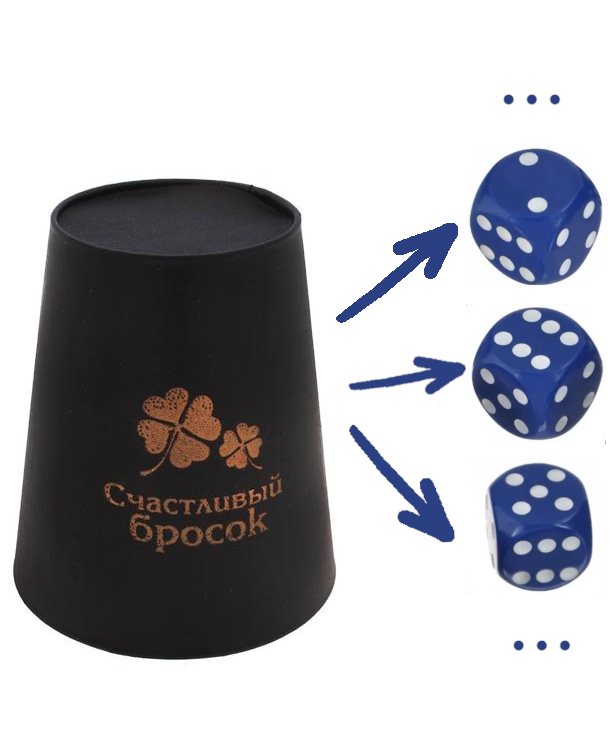
\includegraphics[height=1\textheight]{sample.png}
        \end{center}
    }
\end{frame}

\begin{frame}{Выборка}
    \begin{multicols}{2}
        \begin{center}
            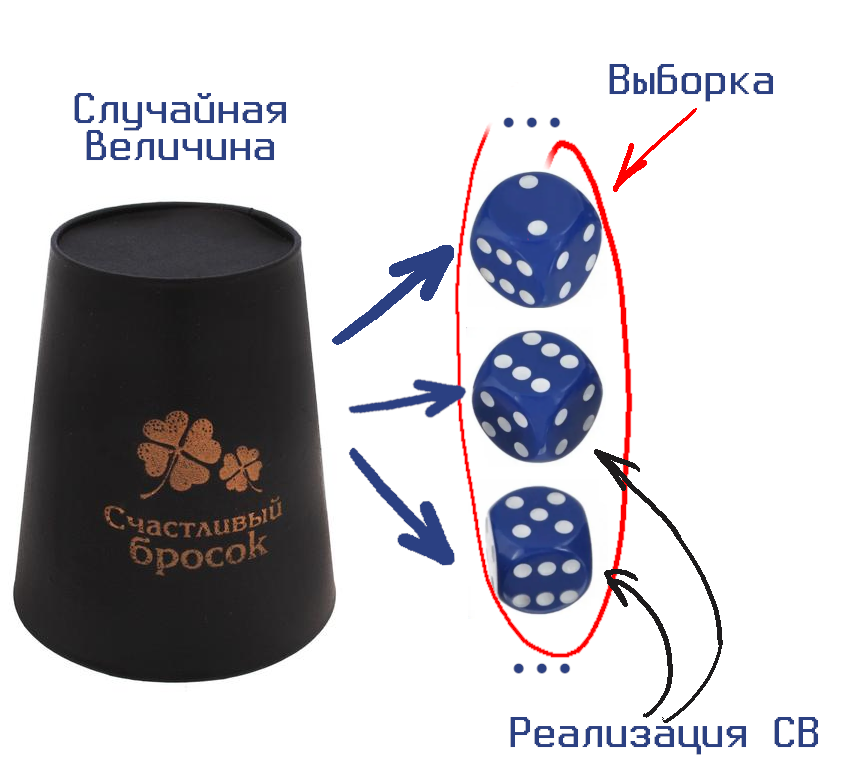
\includegraphics[height=0.8\textheight]{СВ.png}
        \end{center}

        \begin{itemize}
            \item \structure{Реализация СВ} --- выпавшее значение при конкретном броске
            \item \structure{Выборка} --- множество наблюдаемых реализаций
        \end{itemize}
    \end{multicols}
\end{frame}


\begin{frame}{Изучение случайности}
    \alert{Цель теории вероятностей}~---  ограничение сферы действия случайности.

    \begin{multicols}{2}
        \begin{center}
            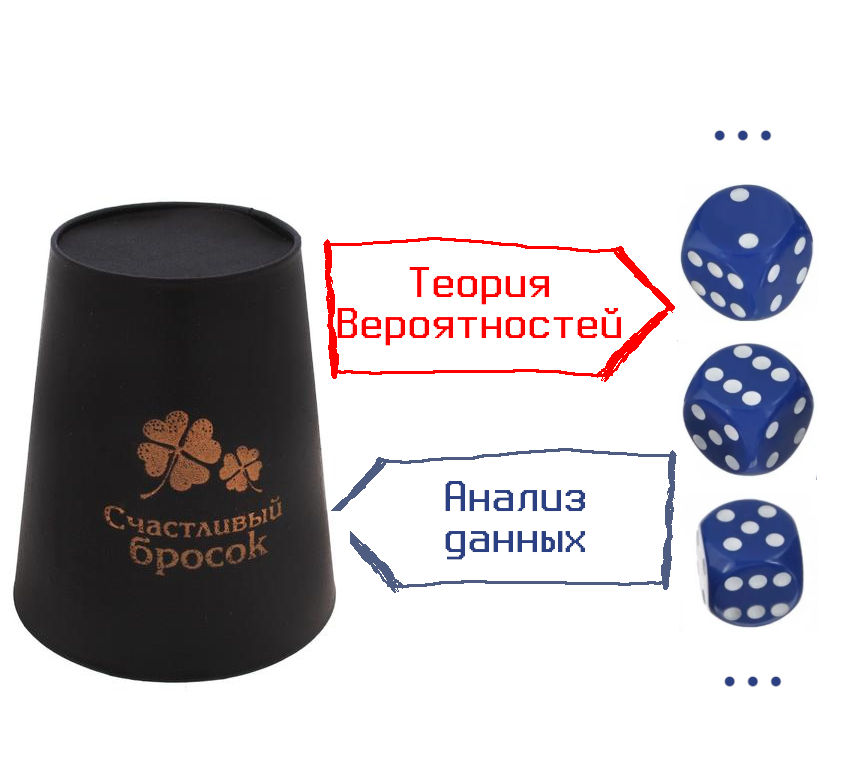
\includegraphics[height=0.7\textheight]{ТВ.png}
        \end{center}
        \columnbreak
        \begin{itemize}
            \item \structure{\bfseries Вероятность события }~---  доля испытаний, завершившихся наступлением события, в бесконечном эксперименте:
            $$
            \prob(A) =  \lim_{n \to +\infty} \frac{n(A)}{n}
            $$
            \item \structure{\bfseries Закон больших чисел}: на больших выборках частота события хорошо приближает его вероятность.
        \end{itemize}
    \end{multicols}
    \alert{Задача статистики:} описание СВ по реализации выборки.


\end{frame}

\begin{frame}{Дискретная случайная величина}{Описание случайных величин}

\structure{Дискретная случайная величина~$X$}, принимает счётное множество значений
$$
    A = \left\{a_1,a_2,\ldots \right\}
$$
с вероятностями
$$
    p_1=\prob(X=x_1), p_2=\prob(X=x_2),\dots,
$$
$$
    \sum\limits_{i} p_i = 1
$$
\begin{multicols}{2}
    \structure{Функция вероятности}

    $$
        f_X(x) = \prob\left( X = x \right)
    $$
    \structure{Функция распределения}

    $$
        F_X(x) = \prob(X \leqslant x )
    $$
\end{multicols}
\end{frame}
\begin{frame}{Непрерывная случайная величина}{Случайные величины}

\begin{multicols}{2}
    \structure{Функция распределения}
    $$
        F_X(x) = \prob(X \leqslant x )
    $$

    \bigskip
    \begin{itemize}
    \item $F_X(x)$ непрерывна
    \item $F_X(x)$ кусочно дифференцируема
    \item  $0 \leqslant F_X(x)\leqslant 1$
    \item  $x_1 < x_2 \Rightarrow F_X(x_1) \leqslant F_X(x_2)$
    \item  $\lim\limits_{x\to -\infty} F_X(x) = 0$
    \item  $\lim\limits_{x\to +\infty} F_X(x) = 1$
    \end{itemize}
    \structure{Стандартное обозначение:} \alert{\texttt{cdf(x)}}
    \columnbreak

    \structure{Функция плотности распределения}
    $$
        f_X(x) = \frac{d}{dx}F_X(x)
    $$

    \bigskip
    \begin{itemize}
        \item $\lim\limits_{x\to \pm\infty} f_X(x) = 0$
        \item $\int\limits_{-\infty}^{+\infty}f_X(x)dx = 1$
        \item $F_X(x) = \int\limits_{-\infty}^{x}f_X(x)dx$
    \end{itemize}
    \structure{Стандартное обозначение:} \alert{\texttt{pdf(x)}}
\end{multicols}
%    или \textbf{плотности распределения}:
%$$f_X\!\left(x\right)\colon \int\limits_a^b f_X\!\left(x\right) dx = \prob\left(a\leq X \leq b\right).$$

\end{frame}


\begin{frame}{Метрические числовые характеристики}{Числовые характеристики распределений}
	\begin{itemize}
		\item \structure{Математическое ожидание}~--- среднее значение $X$:
		$$
            \EE{X} = \int\limits_{-\infty}^{+\infty} x \,dF_X(x) = \int\limits_{-\infty}^{+\infty} x f_X(x)dx, \quad\text{или}\quad \EE{X} = \sum_i x_ip_i
        $$
		\item \structure{Дисперсия}~--- средний квадарат отклонения~$X$ мера разброса $X$:
		$$
            \DD(X) = \EE\left(\left(X-\EE{X}\right)^2\right)
        $$
        \item \structure{Среднее квадратическое отклонение:}
        $$
            \sigma = \sqrt{\DD(X)}
        $$
        \hrule
        \item \structure{Граничный момент порядка $k$}: $\nu_k = \EE(X^k)$
        \item \structure{Центральный момент порядка $k$}: $\mu_k = \EE\left( \left(X-\EE{X}\right)^k\right)$
   \end{itemize}
\end{frame}
\begin{frame}{Мода}{Числовые характеристики распределений}
    \structure{Мода}~--- точка максимума функции вероятности или плотности:
    $$
    \mmode X = \argmax{x} f_X(x)
    $$
\end{frame}
\begin{frame}{Коэффициент асимметрии (skewness)}{Числовые характеристики распределений}
	$$
        \alert{\gamma_1(X) = \EE\left( \frac{X-\EE{X}} {\sigma(X)} \right)^3}
    $$
    \bigskip
	\begin{center}
		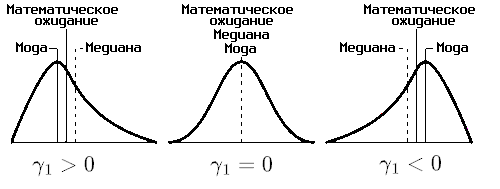
\includegraphics[width=0.8\textwidth]{Skewness.png}
	\end{center}
%    \pause
%    При выраженной асимметрии стандартные процедуры статистического вывода приведут к неравным вероятностям ошибок с каждой стороны!
\end{frame}
\begin{frame}{Коэффициент асимметрии (skewness)}{}

    \begin{center}
        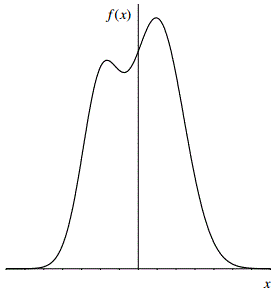
\includegraphics[height=0.7\textheight]{Capture.png}
    \end{center}

    $\gamma_1(X)=0$~--- необходимое, но не достаточное условие симметричности:

\end{frame}
\begin{frame}{Коэффициент эксцесса}{Числовые характеристики распределений}
    \begin{itemize}
        \item $\kurt(X) =  \EE\left( \frac{(X-\EE{X})}{\sigma(X)}\right)^4$~--- куртозис (kurtosis),  эксцесс Фишера
        \item $\alert{\gamma_2(X) = \kurt(X)-3}$~--- \structure{эксцесс Пирсона}, избыточный куртозис
    \end{itemize}
	\begin{center}
		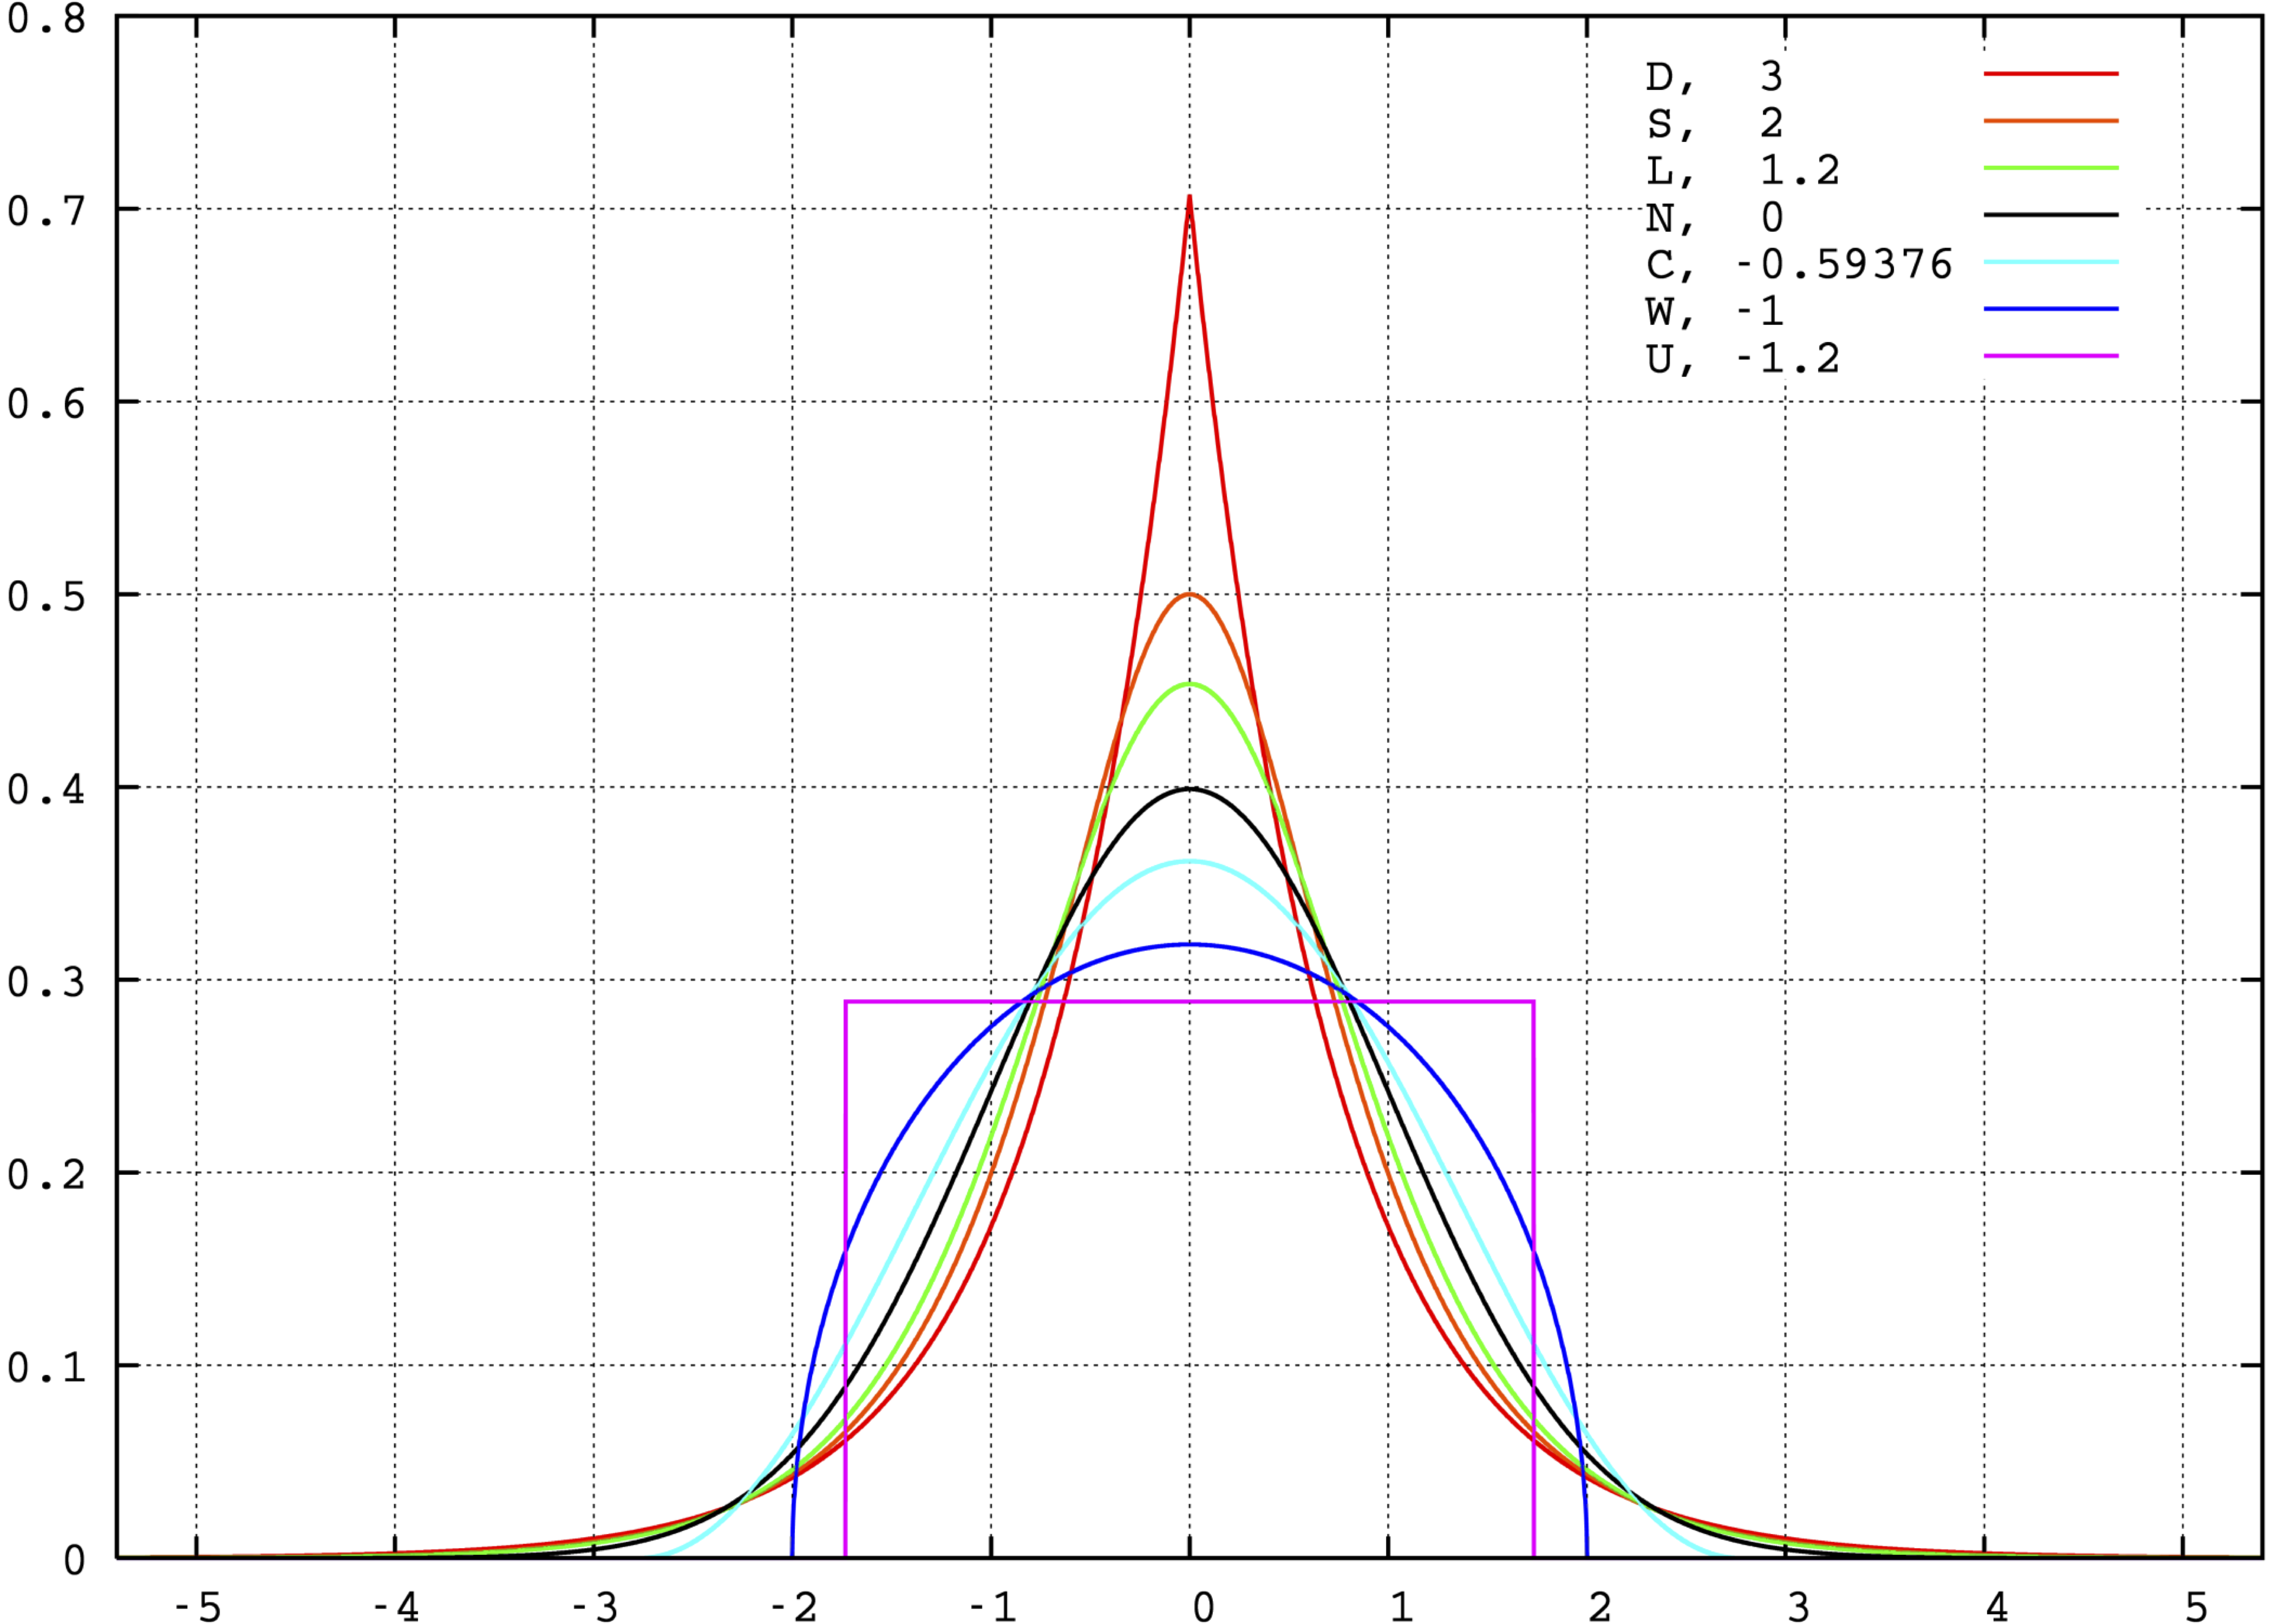
\includegraphics[width=0.5\textwidth]{kurtosis.png}
	\end{center}
\end{frame}




\begin{frame}{Квантили}{Порядковые числовые характеристики распределений}

    Квантильная или процентильная функция --- функция обратная функции распределения.

        \structure{Квантиль} порядка $\alpha\in\left(0,1\right)$:
        $$
        \alert{X_\alpha=F^{-1}\left(\alpha\right)=\inf \lbrace x : F\left(x\right) \geqslant \alpha \rbrace}
        \quad\Longleftrightarrow\quad
        X_\alpha \colon
        \begin{cases}
            \prob\left(X\leqslant X_\alpha\right) \geqslant \alpha, \\
            \prob\left(X\geq X_\alpha\right) \geqslant 1-\alpha
        \end{cases}
        $$
    \structure{Стандартное обозначение:} \alert{$X_\alpha = \;$\texttt{ppf($\alpha$)}}
\end{frame}

\begin{frame}{Квартили}{}
    \structure{Связанные характеристики}:
    \begin{itemize}
        \item Нижний квартиль: $Q_1 = X_{0.25}$
        \item Медиана (центральный квартиль): $Q_2 = X_{0.50}$
        \item Верхний квартиль: $Q_3 = X_{0.75}$
        \item Интерквартильный размах: $IQR = Q_3-Q_1$
    \end{itemize}

    \bigskip
    \hrule

    \medskip
    %%%%%%%%%%%%%%%%%%%%%%%%%%%%%%%%%%%%%%%%%%%%%%%%%%%%%%%%%%%%%%%%%%%%%%%
    % Boxplot состоит из прямоугольника — ящика — и торчащих из него усов. Черта в середине прямоугольника соответствует выборочной медиане. Ширина ящика равна интерквартильному размаху, то есть, его нижняя граница — это 25%-й квантиль, а верхняя — 75%-й квантиль. Длина усов составляет 1.5 интерквартильных размаха, однако в разных реализациях кончик уса может рисоваться в разных местах. Так, на предыдущем слайде усы обрезаются так, что их конец соответствует последнему элементу выборки в этом направлении. Два кружочка на верхнем графике — это объекты выборки, не попавшие в диапазон 4 интерквартильных размаха.
    %%%%%%%%%%%%%%%%%%%%%%%%%%%%%%%%%%%%%%%%%%%%%%%%%%%%%%%%%%%%%%%%%%%%%%%

    \structure{Ящик с усами} (boxplot)~--- способ визуализации распределения в терминах квартилей:
    \begin{figure}
        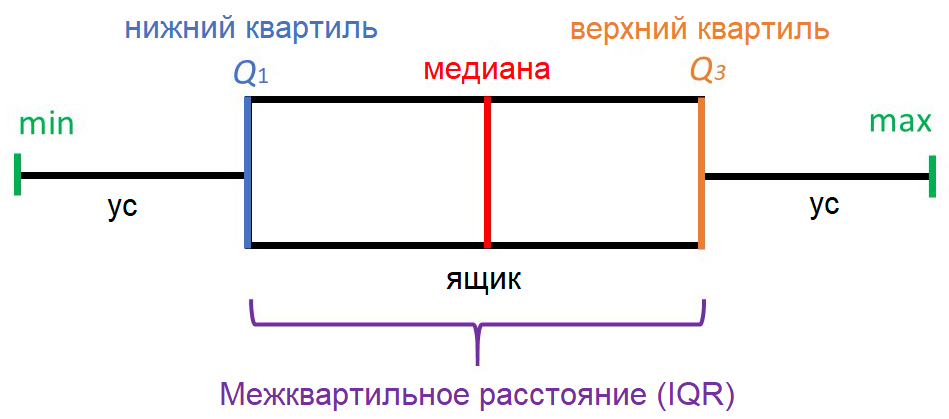
\includegraphics[width=0.5\textwidth]{boxplot_lite.png}
    \end{figure}
    Длина усов отличается в разных реализациях.
\end{frame}


\section{Одномерные распределения}
\subsection{Непрерывные распределения}
\begin{frame}{Нормальное распределение}{\texttt{scipy.stats.norm}}

    $$X\in \RR \sim N\left(\mu, \sigma^2\right), \; \sigma^2>0$$
    \begin{center}
        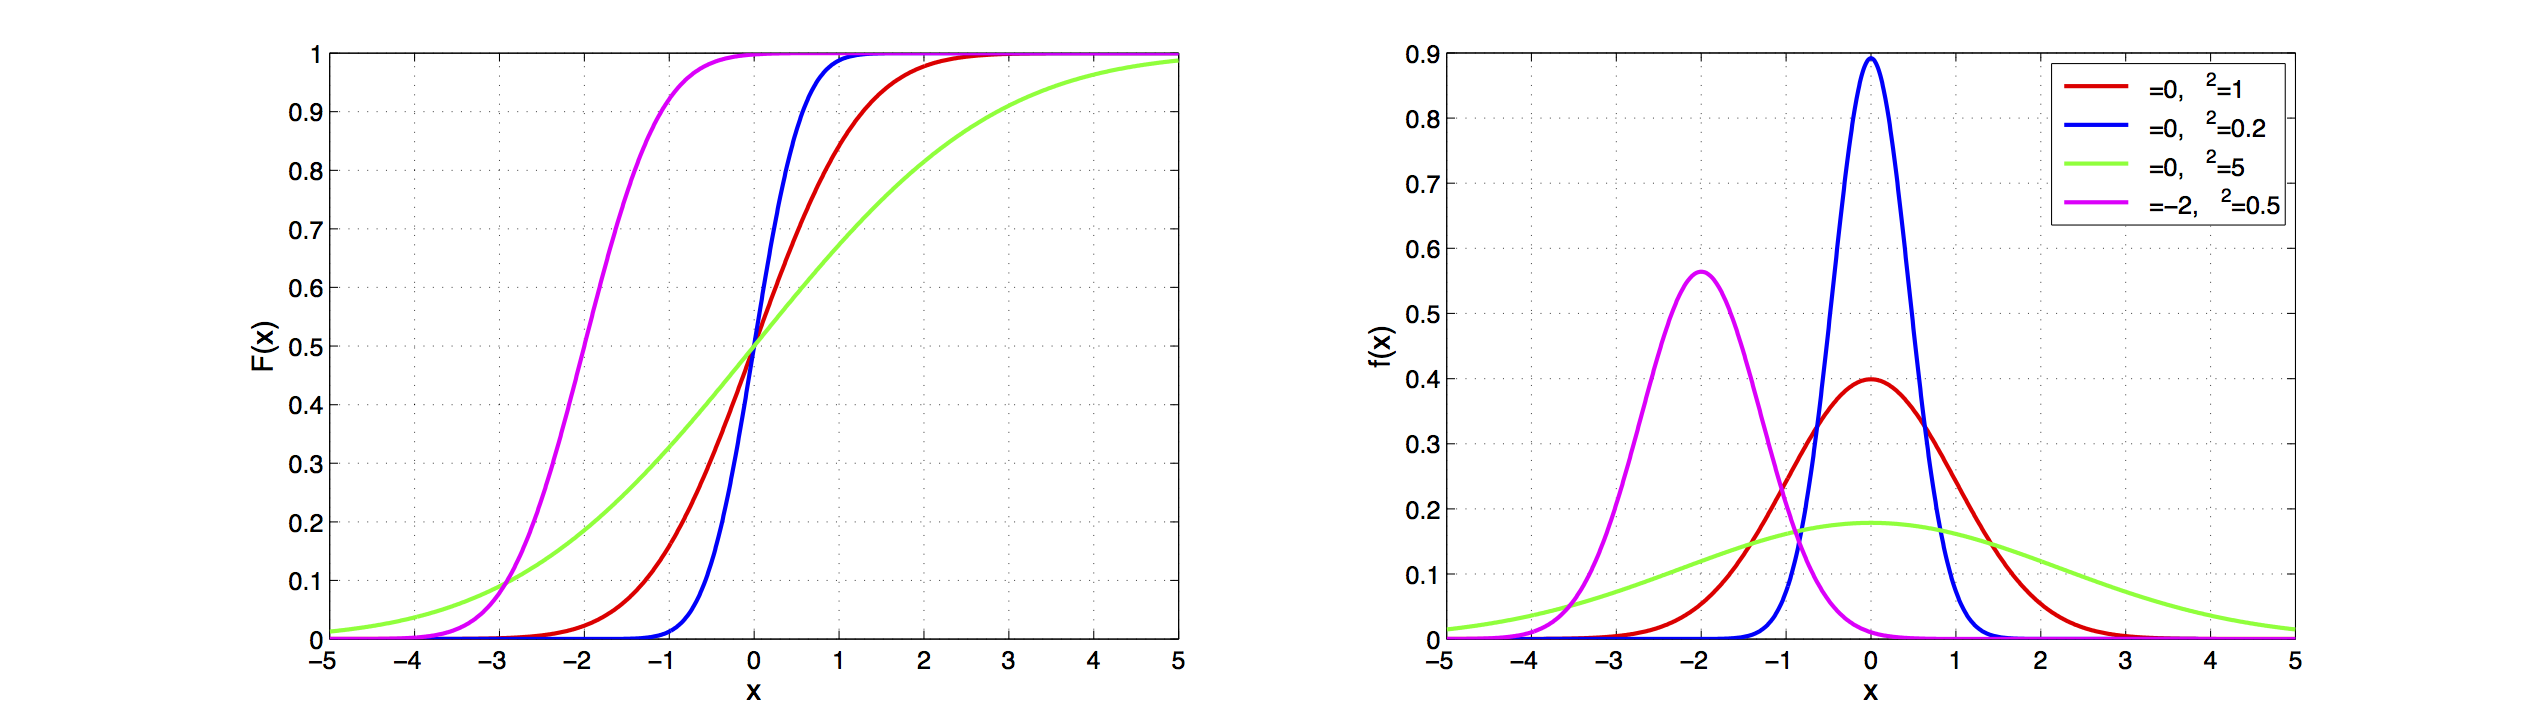
\includegraphics[width=\textwidth]{norm.png}
    \end{center}
    \begin{align*}
         F\left(x\right) &= \Phi\left(\frac{x-\mu}{\sigma}\right)                &\Phi\left(x\right) &= \frac1{\sqrt{2\pi}} \int_{-\infty}^x e^{-\frac{t^2}{2}} dt\\
         f\left(x\right) &= \frac1{\sigma}\phi\left(\frac{x-\mu}{\sigma}\right)  &\phi\left(x\right) &= \frac1{\sqrt{2\pi}} e^{-\frac{x^2}{2}}\\
    \end{align*}
\end{frame}
\begin{frame}{Нормальное распределение}{Свойства}
	\begin{itemize}
	    \item предельное распределение суммы слабо взаимозависимых СВ
	    \item $\EE{X} = \med X = \mmode X = \mu$, $\DD{X}  = \sigma^2$,  все моменты более высокого порядка нулевые
    	\item Пусть $X_1,\dots,X_n$ независимы, \; $X_i\sim N\left(\mu_i, \sigma_i^2\right),$ тогда $\forall a_1,\dots,a_n$
    	$$\sum\limits_{i=1}^n a_i X_i \sim N\left(\sum_{i=1}^n a_i \mu_i, \sum_{i=1}^n a_i^2 \sigma_i^2\right)$$
    	\item Центральная предельная теорема: пусть $X_1,\dots,X_n$ i.i.d. с $\EE{X}$ и $\DD{X}<\infty$, тогда
    	$$\frac1{n}\sum_{i=1}^n X_i \approx N\left(\EE{X}, \frac{\DD{X}}{n}\right)$$
    \end{itemize}
\end{frame}

\begin{frame}{Распределение Реллея}{\texttt{scipy.stats.rayleigh}}
$X,Y$~--- независимые СВ.
$$
X\sim N(0,\sigma^2),\qquad Y\sim N(0,\sigma^2), \qquad R=\sqrt{X^2+Y^2}
$$
$$
    R\sim \mathrm {Rayleigh} (\sigma )
$$
\begin{center}
    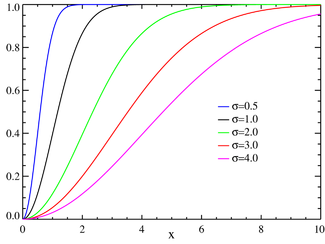
\includegraphics[width=0.35\textwidth]{RayleighCDF.png}      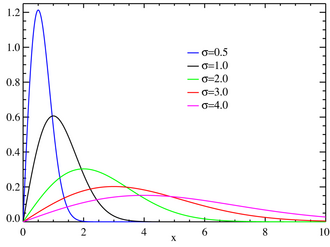
\includegraphics[width=0.35\textwidth]{RayleighPDF.png}
\end{center}
$$
F(x, \sigma )=1-e^{-x^{2}/(2\sigma^{2})},\qquad f(x,\sigma )={\frac {x}{\sigma ^{2}}}e^{-x^{2}/(2\sigma ^{2})},\quad x\geqslant 0
$$


\end{frame}

\begin{frame}{Распределение хи-квадрат}{\texttt{scipy.stats.chi2}}
 \only<1>{
    \begin{itemize}
    \item пусть $X_1,\dots,X_k$~--- i.i.d., \; $X_i\sim N\left(0,1\right),$ тогда
    $$\sum\limits_{i=1}^k X_i^2 \sim \chi^2_k$$
    \item пример: нормированная выборочная дисперсия: $$(n-1)\frac{S_n^2}{\sigma^2}\sim \chi^2_{n-1}$$
    \end{itemize}
    }

    \only<2>{
    $$
        X\in \RR_+ \sim \chi^2_k, \; k\in\NN 
    $$

    \begin{center}
    	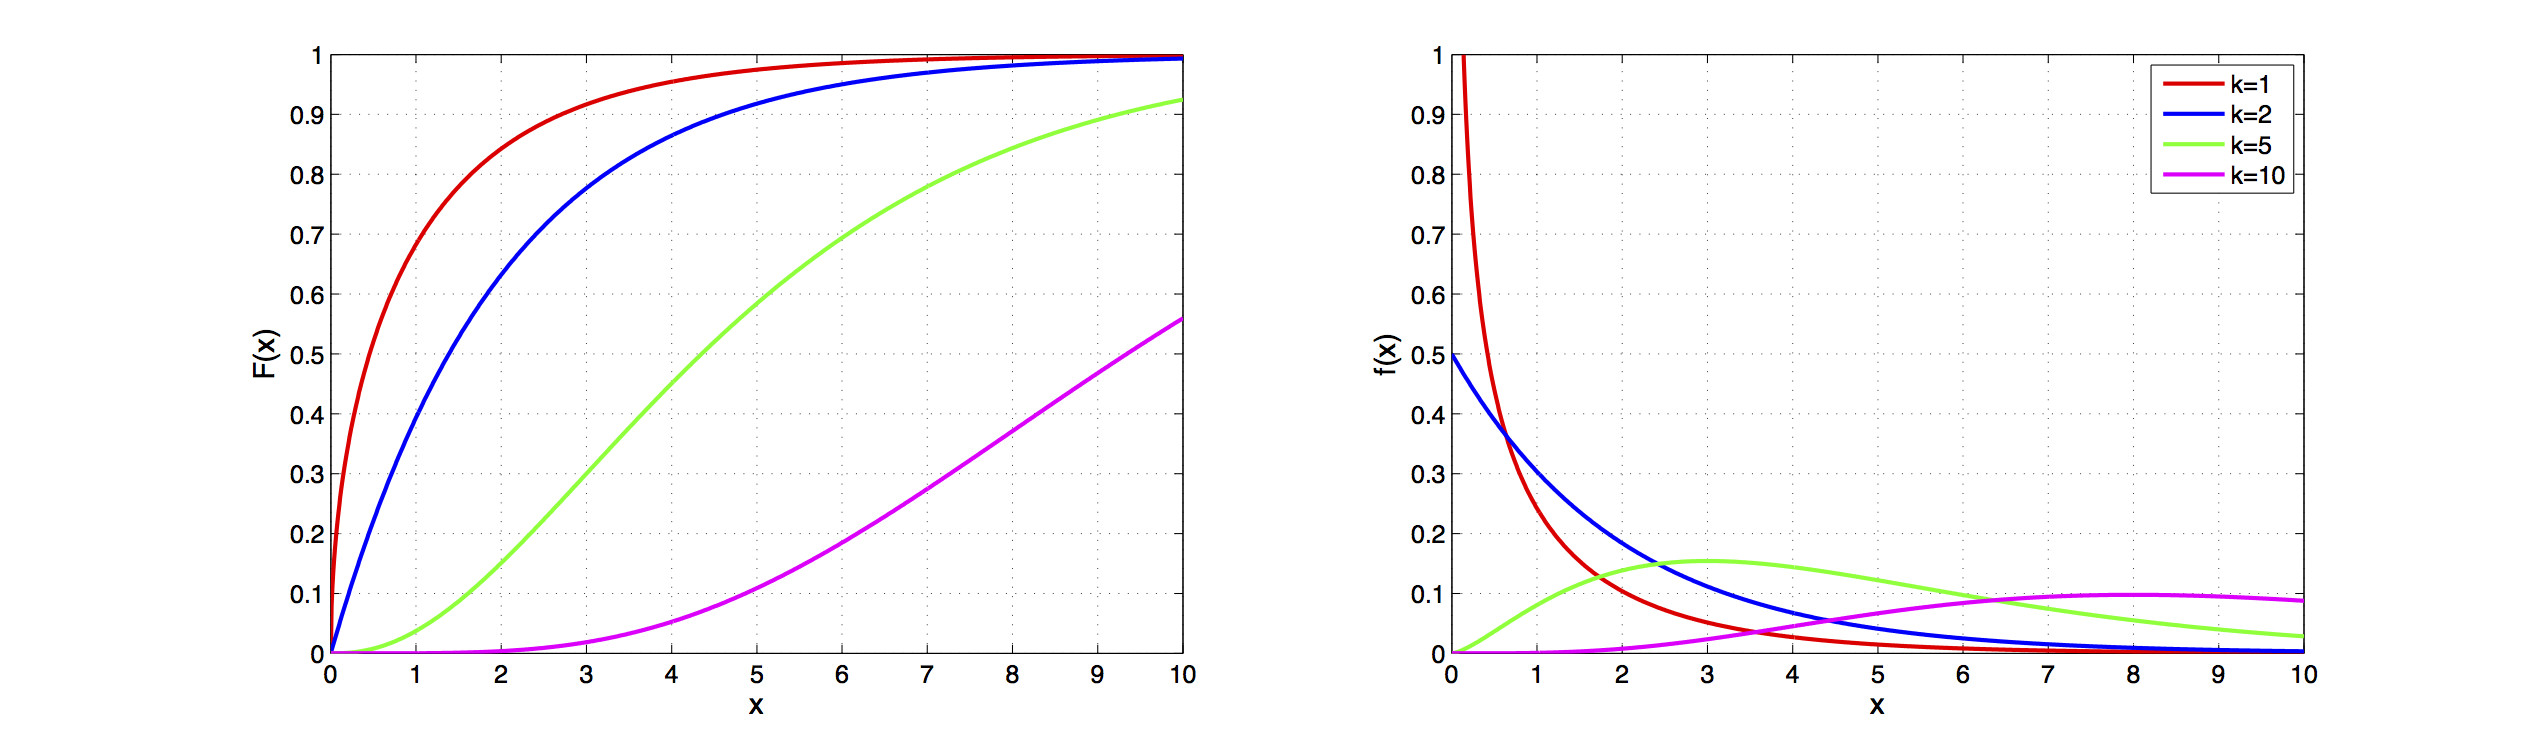
\includegraphics[width=\textwidth]{chi2.png}
    \end{center}
    $$
         F\left(x\right)        = \frac1{\Gamma\left(\frac{k}{2}\right)}\gamma\left(\frac{k}{2}, \frac{x}{2}\right),\qquad
         f\left(x\right)        = \frac1{2^{\frac{k}{2}}\Gamma\left(\frac{k}{2}\right)}x^{\frac{k}{2}-1}e^{-\frac{x}{2}}
    $$

	{\small
    $\Gamma\left(x\right) = \int_0^{\infty} t^{x-1} e^{-t} dt$~--- гамма"=функция

    $\gamma\left(a,x\right) = \int_0^x e^{-t} t^{a-1} dt$~--- нижняя неполная гамма"=функция
	}
    }


\end{frame}


\begin{frame}{Распределение Фишера}{\texttt{scipy.stats.f}}
%%%%%%%%%%%%%%%%%%%%%%%%%%%%%%%%%%%%%%%%%%%%%%%%%%%%%%%%%%%%%%%%%%%%%%%
% Распределение Фишера может выглядеть очень по-разному при разных значениях своих параметров.
%%%%%%%%%%%%%%%%%%%%%%%%%%%%%%%%%%%%%%%%%%%%%%%%%%%%%%%%%%%%%%%%%%%%%%%

    \only<1>{
    \begin{itemize}
    \item пусть $X_1\sim\chi^2_{d_1},$\; $X_2\sim\chi^2_{d_2},$  \; $X_1$ и $X_2$ независимы, тогда
    $$\frac{X_1/d_1}{X_2/d_2} \sim F\left(d_1,d_2\right)$$
    \item  если $X\sim F\left(d_1,d_2\right),$ то
    $$Y = \lim_{d_2\rightarrow \infty} d_1X \sim \chi^2_{d_1}$$
    \item $F\left(x,d_1,d_2\right) = F\left(1/x,d_2,d_1\right)$
    \item возникает в дисперсионном и регрессионном анализе
    \end{itemize}
    }

    \only<2>{
    $$
    X\in \RR_+ \sim F\left(d_1,d_2\right), \; d_1,d_2>0
    $$

    \begin{center}
    	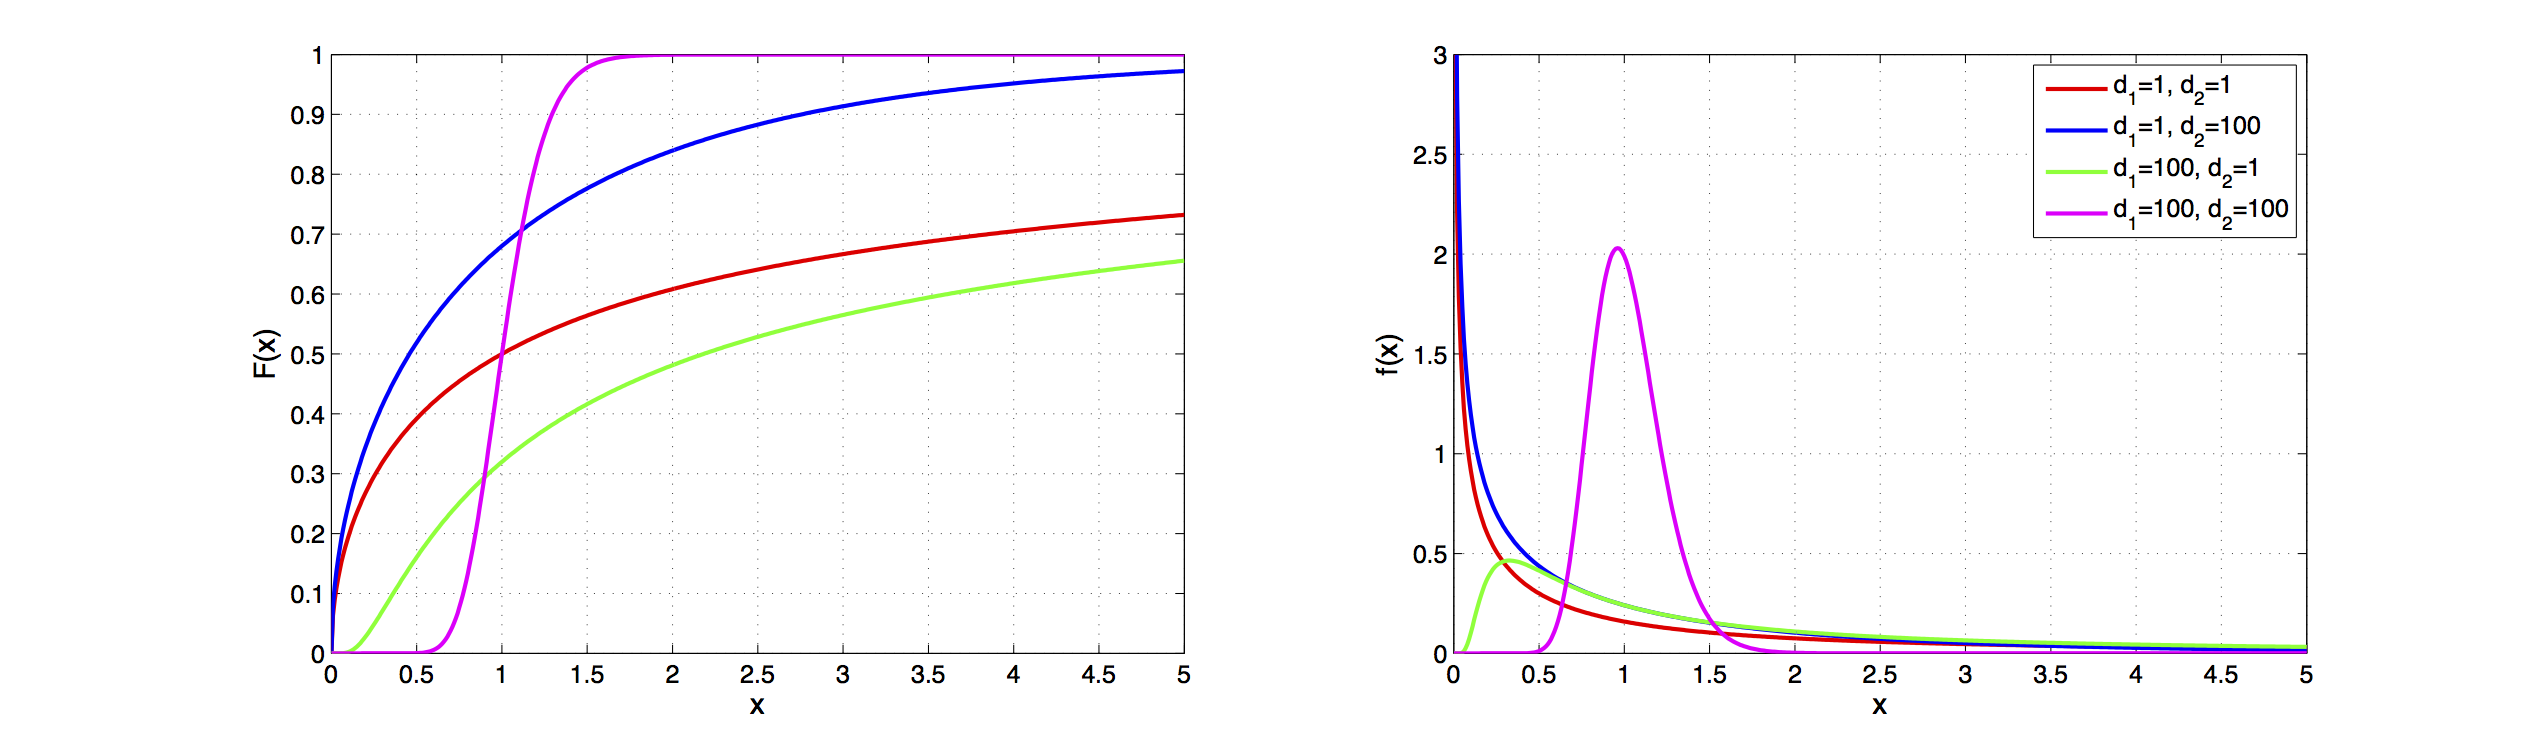
\includegraphics[width=\textwidth]{fish.png}
    \end{center}

    \vspace{-20pt}

    \begin{align*}
         F\left(x\right)        = I_{\frac{d_1 x}{d_1 x + d_2}} \left(\frac{d_1}{2}, \frac{d_2}{2} \right) \qquad
         f\left(x\right)        = \left. \sqrt{\frac{\left(d_1x\right)^{d_1}d_2^{d_2}}{\left(d_1x+d_2\right)^{d_1+d_2}}} \middle/  xB\left(\frac{d_1}{2}, \frac{d_2}{2}\right) \right. \\
    \end{align*}

    \vspace{-20pt}

	{\footnotesize
    $B\left(a,b\right) = \int_0^1 t^{a-1} \left(1-t\right)^{b-1} dt$~--- бета-функция

    $I_x\left(a,b\right) = \frac{B\left(x; a,b\right)}{B\left(a,b\right)}$~--- регуляризованная неполная бета-функция

    $B\left(x; a,b\right) = \int_0^x t^{a-1} \left(1-t\right)^{b-1} dt$~--- неполная бета-функция
	}
    }

\end{frame}

\begin{frame}{Распределение Стьюдента}{\texttt{scipy.stats.t}}
%%%%%%%%%%%%%%%%%%%%%%%%%%%%%%%%%%%%%%%%%%%%%%%%%%%%%%%%%%%%%%%%%%%%%%%
% Распределение Стьюдента похоже на стандартное нормальное - у него всегда нулевое среднее, но хвосты более тяжёлые. Чем больше число степеней свободы, тем меньше отличия - уже начиная с nu=30 визуально отличить из невозможно (эвристика alert!) Как и предыдущие, может определяться с нецелым числом степеней свободы - мы будем этим активно пользоваться в дальнейшем.
%%%%%%%%%%%%%%%%%%%%%%%%%%%%%%%%%%%%%%%%%%%%%%%%%%%%%%%%%%%%%%%%%%%%%%%
    \only<1>{
    \begin{itemize}
    \item $\EE{X} = 0$  при  $\nu>1$, $\med X = \mmode X = 0$ всегда
    \item пусть $Z\sim N\left(0,1\right)$  и $V\sim\chi^2_{\nu}$ независимы, тогда
    $$T = \frac{Z}{\sqrt{V/\nu}} \sim St\left(\nu\right)$$
    \item если $X\sim St\left(\nu\right),$ то
    $$Y = \lim_{\nu\rightarrow\infty} X \sim N\left(0,1\right)$$
    \item возникает при оценке среднего значения СВ с неизвестной дисперсией
    \end{itemize}
    }

    \only<2>{
    $$
        X\in \RR \sim St\left(\nu\right), \; \nu>0
    $$

    \begin{center}
        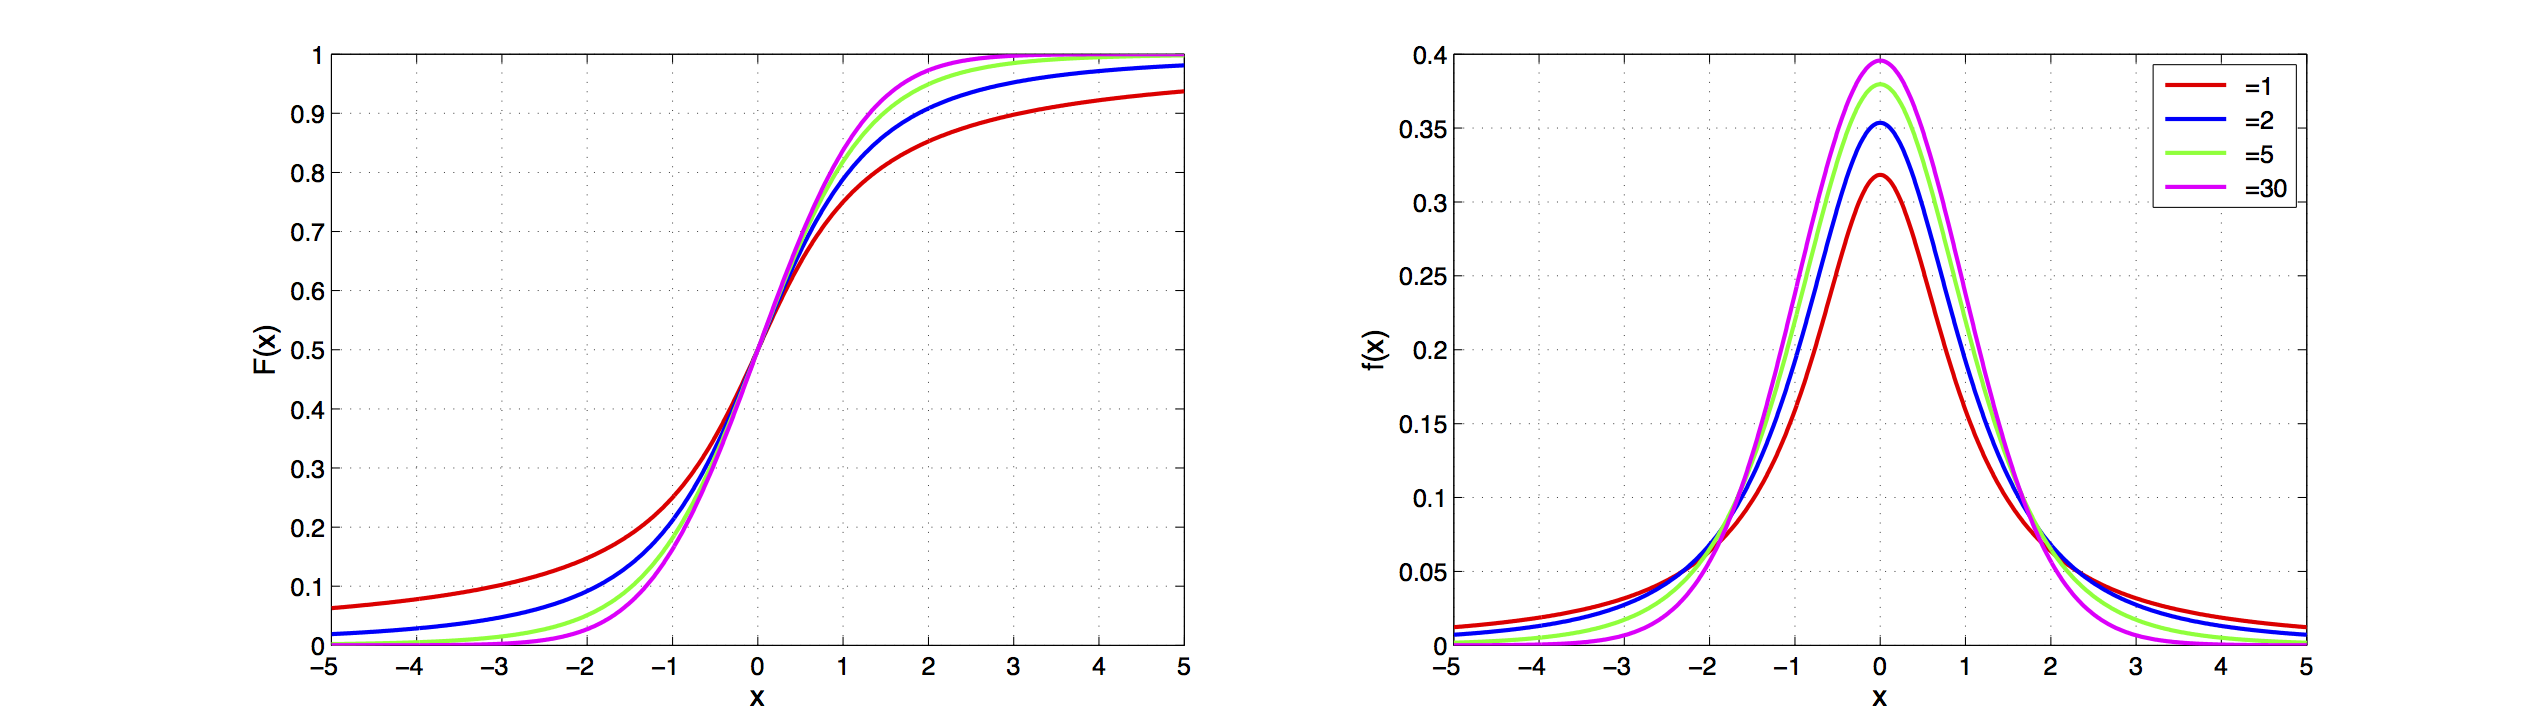
\includegraphics[width=\textwidth]{stud.png}
    \end{center}
    $$
         F\left(x\right) = \frac1{2}+x\Gamma\left(\frac{\nu+1}{2}\right),
         \qquad
         f\left(x\right) = \frac{\Gamma\left(\frac{\nu+1}{2}\right)}{\sqrt{\nu\pi} \Gamma\left(\frac{\nu}{2}\right)} \left(1+\frac{x^2}{\nu}\right)^{-\frac{\nu+1}{2}}
    $$
    }

\end{frame}


\subsection{Дискретные распределения}
\begin{frame}{Распределение Бернулли}{\texttt{scipy.stats.bernoulli}}
%%%%%%%%%%%%%%%%%%%%%%%%%%%%%%%%%%%%%%%%%%%%%%%%%%%%%%%%%%%%%%%%%%%%%%%
%
%%%%%%%%%%%%%%%%%%%%%%%%%%%%%%%%%%%%%%%%%%%%%%%%%%%%%%%%%%%%%%%%%%%%%%%
    \only<1>{
    $$X\in \left\{0, 1\right\} \sim Ber\left(p\right), \;\; p \in \left(0,1\right)$$

%
    \begin{center}
    	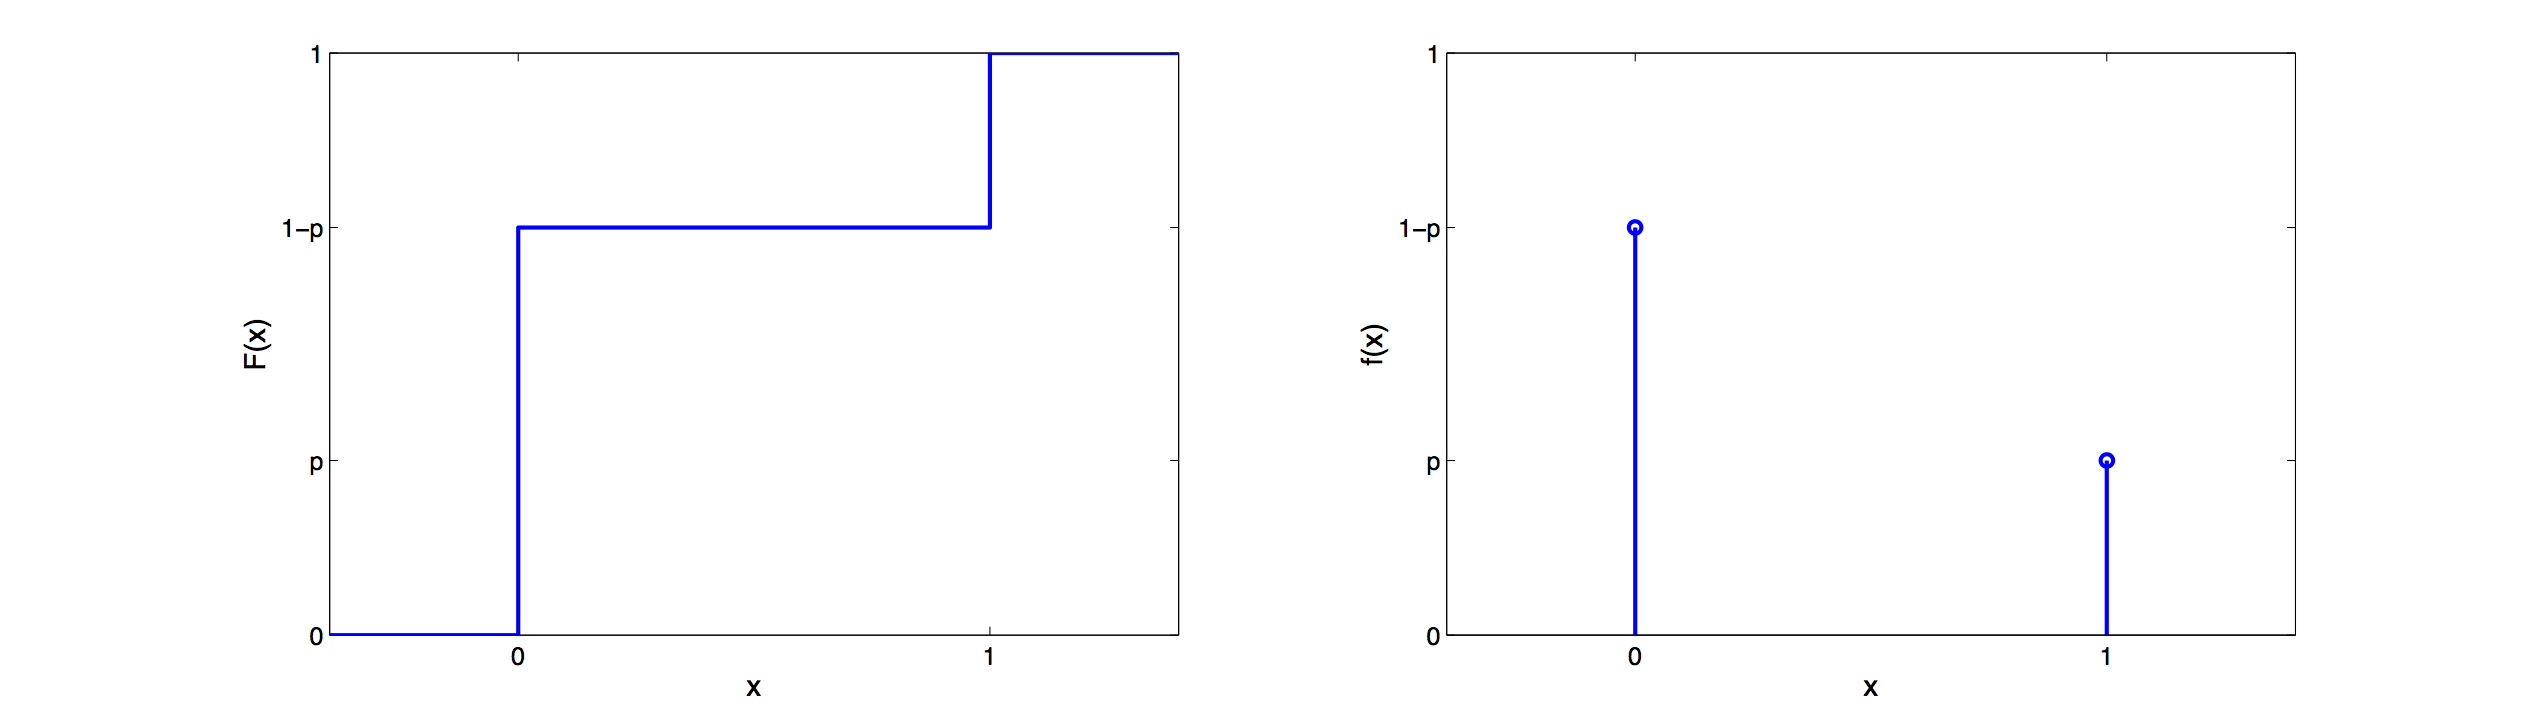
\includegraphics[width=0.8\textwidth]{ber.png}
    \end{center}

\vspace{-10pt}

    $$
        F\left(x\right)   = \begin{cases}
                            0, & x<0, \\
                            1-p, & 0\leq x<1, \\
                            1, & x\geq 1.
                        \end{cases}
        \qquad    
         f\left(x\right)  = \begin{cases}
                            1-p, & x=0, \\
                            p,   & x=1.
                        \end{cases}
    $$

\vspace{-10pt}

    \begin{itemize}
  	\item пример: результат подбрасывания монеты
    \end{itemize}
    }
\end{frame}

\begin{frame}{Биномиальное распределение}{\texttt{scipy.stats.binoois}}
%%%%%%%%%%%%%%%%%%%%%%%%%%%%%%%%%%%%%%%%%%%%%%%%%%%%%%%%%%%%%%%%%%%%%%%
%
%%%%%%%%%%%%%%%%%%%%%%%%%%%%%%%%%%%%%%%%%%%%%%%%%%%%%%%%%%%%%%%%%%%%%%%
    \only<1>{
    $$X\in \left\{0, \dots,N\right\} \sim Bin\left(N,p\right), \; N \in \NN, \;\; p\in\left[0,1\right]$$

    \begin{center}
        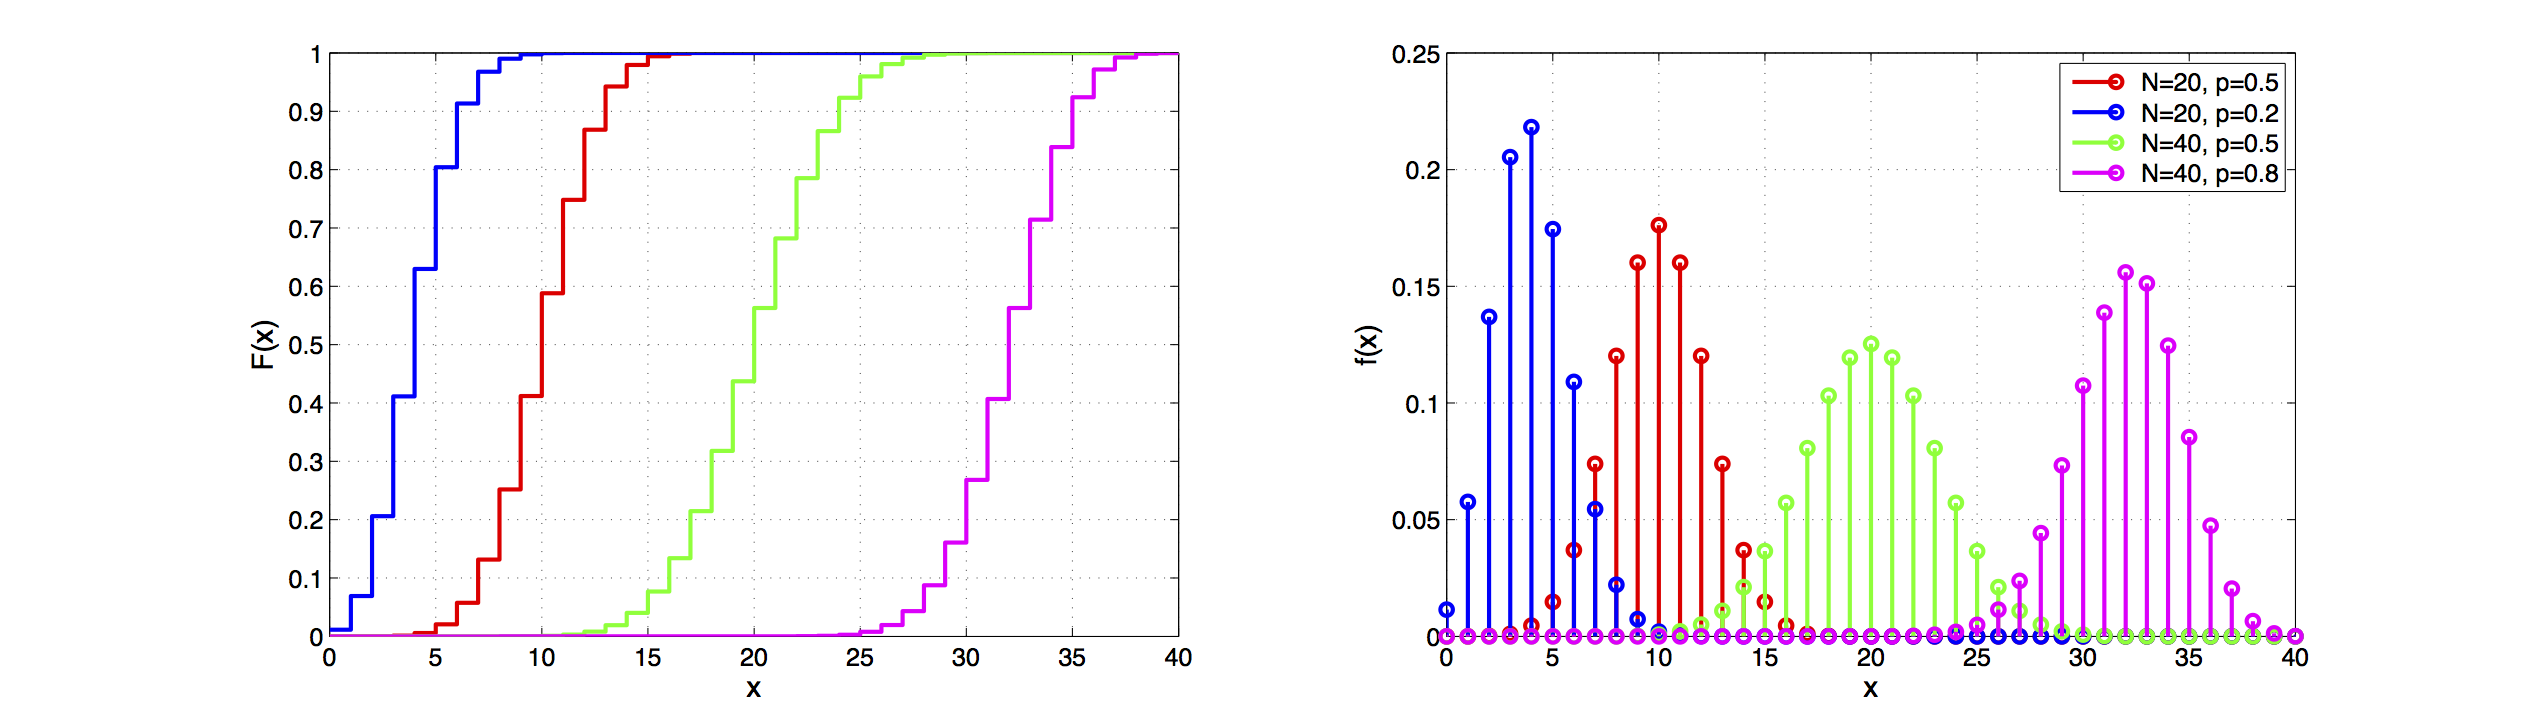
\includegraphics[width=\textwidth]{bin.png}
    \end{center}
    $$
    F\left(x\right) = I_{1-p}\left(N-x, 1+x\right),
    \qquad
    f\left(x\right) = C_N^x p^x \left(1-p\right)^{N-x} 
    $$
    }

	\only<2>{
    \begin{itemize}
    \item пусть $X_1,\dots,X_n$ независимы, $X_i\sim Ber(p)$, тогда $$\sum_{i=1}^n X_i \sim Bin(n,p).$$
    \item $Bin\left(1,p\right) = Ber\left(p\right)$
    \item если $N>20$ и $p$ не слишком близко к нулю или единице, то для $X\sim Bin\left(N,p\right)$ справедлива нормальная аппроксимация:
    $$F_X\left(x\right) \approx \Phi \left(\frac{x-Np}{\sqrt{Np\left(1-p\right)}}\right)$$
    \item пример: число попаданий из $N$ бросков в баскетбольное кольцо
    \end{itemize}
    }
\end{frame}
\begin{frame}{Распределение Пуассона}{\texttt{scipy.stats.poisson}}
%%%%%%%%%%%%%%%%%%%%%%%%%%%%%%%%%%%%%%%%%%%%%%%%%%%%%%%%%%%%%%%%%%%%%%%
% Распределение Пуассона - дефолтное распределение для счётчиков, точно так же как нормальное - для непрерывных случайных величин. Это не значит, что все счётчики описываются этим распределением, а только что его имеет смысл попробовать в первую очередь.
%%%%%%%%%%%%%%%%%%%%%%%%%%%%%%%%%%%%%%%%%%%%%%%%%%%%%%%%%%%%%%%%%%%%%%%
    \only<1>{
    $$X\in \left\{0,1,2,\dots \right\} \sim Pois\left(\lambda\right), \; \lambda>0$$

    \begin{center}
        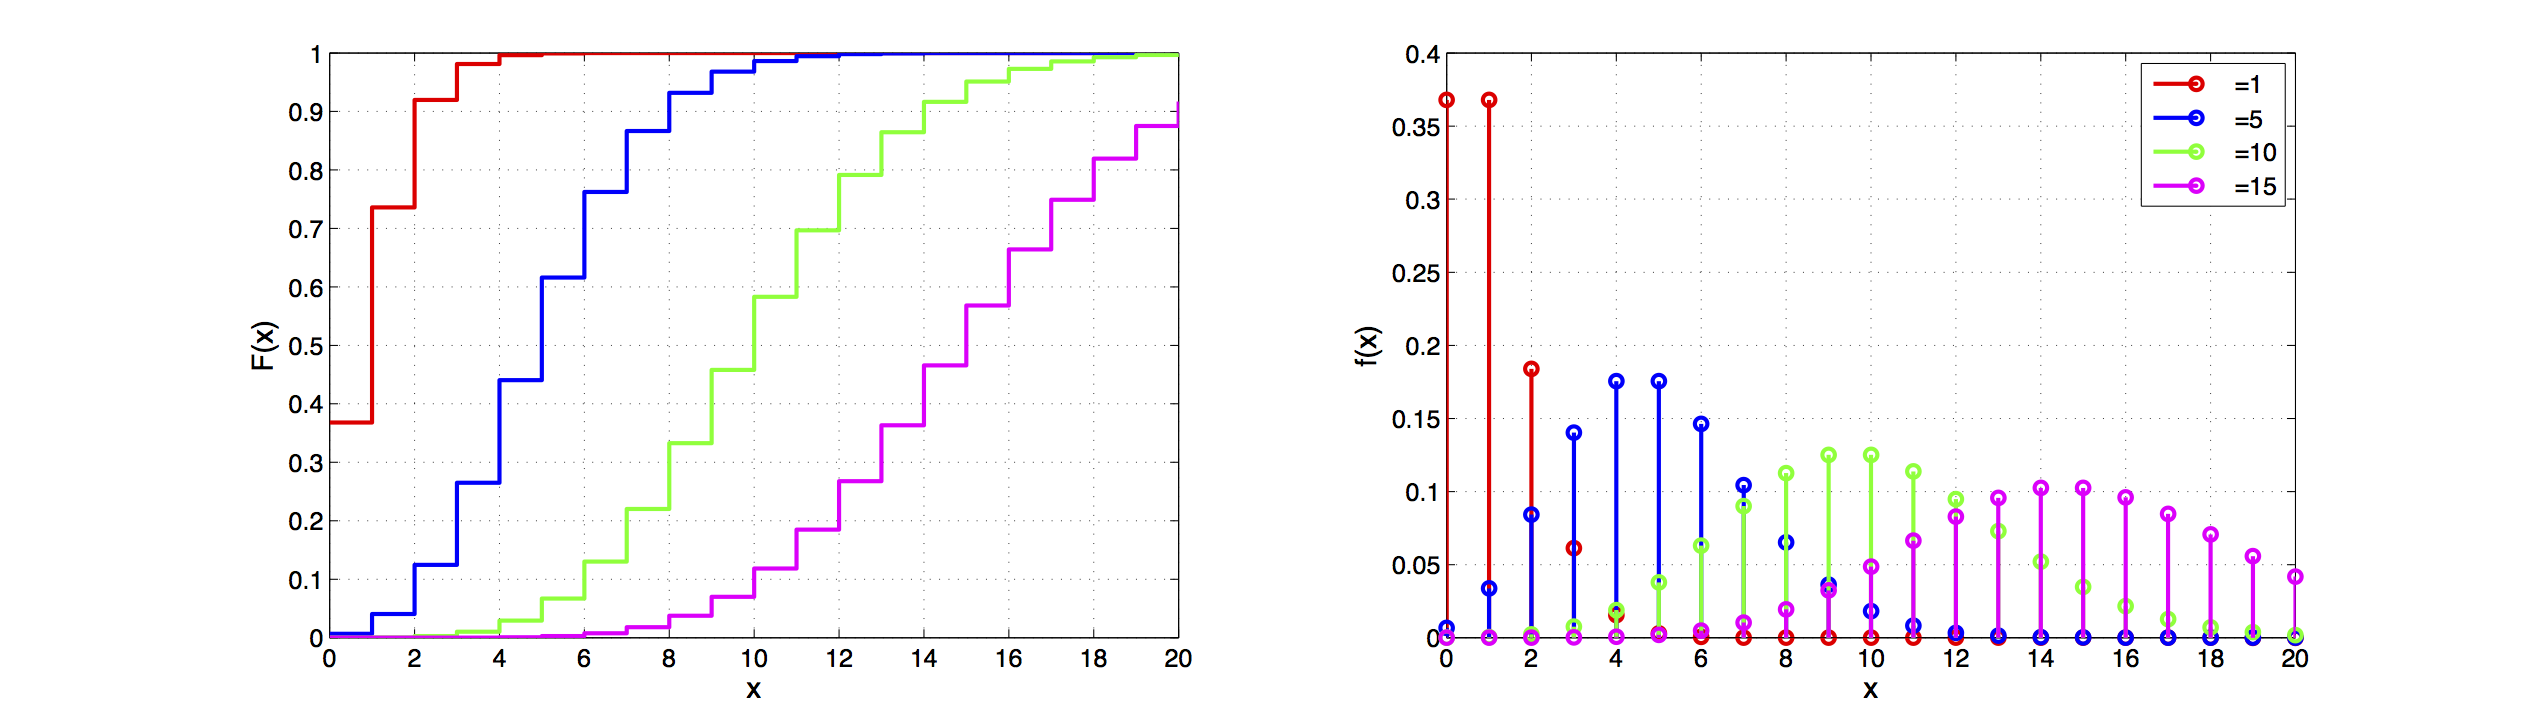
\includegraphics[width=\textwidth]{poiss.png}
    \end{center}
    $$
         F\left(x\right)        = e^{-\lambda}\sum\limits_{i=0}^{\lfloor x\rfloor} \frac{\lambda^i}{i!},
         \qquad
         f\left(x\right) = e^{-\lambda} \frac{\lambda^x }{x!}
    $$
    }

    \only<2>{
    \begin{itemize}
	    \item распределение числа независимых событий в~фиксированном временном или пространственном интервале
	    \item $\EE{X} = \DD{X} = \lambda$
    	\item пусть $X_1,\dots,X_n$ независимы, \; $X_i\sim Pois\left(\lambda_i\right),$ тогда
    	$$\sum\limits_{i=1}^n X_i \sim Pois\left(\sum_{i=1}^n \lambda_i\right)$$
    	\item если $X\sim Pois\left(\lambda\right),$ $Y=\sqrt{X},$  то при больших $\lambda$ $$F_Y\left(x\right)\approx \Phi\left(\frac{x-\sqrt{\lambda}}{\sqrt{\lambda}}\right)$$
    	\item  $Bin(n,p) \xrightarrow{n \to \infty} Pois(\lambda)$ при постоянном $\lambda = np$
    	\item Пример: количество изюма в булочке с изюмом
    \end{itemize}
    }
\end{frame}



\section{Статистики}
\begin{frame}{}
\centering
\huge Статистика
\end{frame}

\subsection{Выборка и статистика}
\begin{frame}{Основные понятия}
    \structure{Генеральная совокупность}~--- множество объектов, свойства которых подлежат изучению в рассматриваемой задаче.

    \bigskip

    \structure{Выборка}~--- конечное множество объектов, отобранных из генеральной совокупности для проведения измерений.
    $$
        X^n=\left(X_1,\dots,X_n\right).
    $$

    \bigskip
    \structure{Виды выборок:}
    \begin{itemize}
    \item \structure{пространственная выборка ($X^n$)}~--- $X_1,\dots,X_n$~--- независимые одинаково распределённые случайные величины (i.i.d.). Порядок следования наблюдений неважен.
    \item \structure{временная выборка}~--- $X_1,\dots,X_n$~--- зависимые случайные величины. Порядок следования наблюдений важен.
    \end{itemize}
    \bigskip



\end{frame}
\begin{frame}{Вариационный ряд}

    \textbf{Вариационный ряд}~--- ранжированная выборка
    $$X_{(1)}\leqslant X_{(2)} \leqslant \dots \leqslant X_{(n)}$$

    \textbf{ранг} элемента выборки $X_i$:
    $$\rank\left(X_i\right)=r\colon X_i=X_{(r)}$$

\end{frame}



\begin{frame}{Интервальный статистический ряд}{}
    $$
    {\color{black}
        \begin{array}{c|cccc}
            x_i & \left(x_0,x_1\right] & \left(x_1,x_2\right] & \cdots & \left(x_{k-1},x_k\right] \\
            \hline
            n_i & n_1 & n_2 & \cdots & n_k \\
        \end{array}
        \qquad \text{где}\quad
    }
    n_1+n_2+\ldots+ n_k=n
    $$
    \medskip
    $$
    {\color{black}
        \begin{array}{c|cccc}
            x_i & \left(x_0,x_1\right] & \left(x_1,x_2\right] & \cdots & \left(x_{k-1},x_k\right] \\
            \hline
            w_i & w_1 & w_2 & \cdots & w_k \\
        \end{array}
        \qquad \text{где}\quad
    }
    w_1+w_2+\ldots+ w_k=1
    $$



    \bigskip

    \begin{itemize}
        \item Число интервалов:  $k = 1+\lfloor \log_{2}{n} \rfloor$ формула Стёрджеса:
        \item Длина интервала вычисляется по формуле:
        $
        h= \frac{x_{\max}-x_{\min}}{k-1}
        $
        \item Расширение размаха вариации:
        $
        x'_{\min}= x_{\min}-\frac{h}{2}
        $
        \item Представитель  интервала $x_i^* = \frac{x_i+x_{i+1}}{2}$.
    \end{itemize}
\end{frame}

\begin{frame}[t,allowframebreaks]{Пример}{}
    \begin{exampleblock}{}
        Измерили рост (с точностью до см) 30 наудачу отобранных студентов:

        153, 154, 155, 155, 156, 157, 158, 159, 160, 163, 164, 165, 166, 167, 167, 169, 170, 171, 171, 172, 173, 173, 175, 175, 178, 179, 179, 182, 183, 186.

        Построить интервальный статистический ряд.
    \end{exampleblock}
    \begin{itemize}
        \item $X$~--- рост студента~--- непрерывная с.\,в.
        \item Данные ранжированы,
        $$
        n = 30, \qquad x_{\min}=153, \qquad x_{\max}=186
        $$
        \item Вычислим количество интервалов:
        $$
        k =  1+ \lfloor\log_2{30} \rfloor = 5
        $$
        \vspace{-5mm}
        \item  Находим длину частичного интервала
        $$
        h = \frac{x_{\max}-x_{\min}}{k} = \left[\frac{186-153}{4}\right] = 8,25 \approx 8
        $$

        \vspace{-2mm}
        \item Расширяем промежуток:
        \begin{align*}
            x'_{\min} &= x_{\min}-\frac{h}{2} = 153-\frac{8}{2} \approx 149\\
        \end{align*}
        \vspace{-4mm}
        \item Строим интервальный ряд:
    \end{itemize}
    $
    \small
    \begin{array}{|c|c|c|c|c|c||c|}
        \hline
        x_i & \left[149; 157 \right) &  \left[157; 165\right) &  \left[ 165; 173 \right) &  \left[ 173; 181 \right) &  \left[181; 189 \right) & \Sigma\\
        \hline
        x^*_i & 153 &  159 &  165 &  171 &  177 &  183 \\
        \hline
        n_i & 5 & 6 & 9 & 7 & 3 & 30\\
        \hline
        w_i & 0,17 & 0,20 & 0,30 & 0,23 & 0,10 & 1\\
        \hline
    \end{array}
    $
\end{frame}



\pgfplotsset{
    compat=newest,
    xlabel near ticks,
    ylabel near ticks
}

\begin{frame}{Гистограмма}{}
%    \begin{block}{Определение}
%        \alert{Гистограмма частостей}~--- cтупенчатая фигура, состоящая из прямоугольников, основаниями которых
%        служат частичные интервалы $\left(x_{i-1};x_i\right]$  длиною $h$, а~высоты равны отношению $\frac{w_i}{h}$~--- плотности частостей.
%    \end{block}
%
%
%    \begin{minipage}{8cm}
%%        \centering\includegraphics[width=7cm]{hist-1.png}
%    \end{minipage}
%    \begin{minipage}{2cm}
%        {\LARGE
%            $$
%            S=1
%            $$
%            \par}
%    \end{minipage}
%\end{frame}
%
%\begin{frame}{Пример гистограммы}{}
    \small
    $
    \setlength{\tabcolsep}{-1pt}
    \begin{array}{|c|c|c|c|c|c||c|}
    \hline
    x_i & \left[149; 157 \right) &  \left[157; 165\right) &  \left[ 165; 173 \right) &  \left[ 173; 181 \right) &  \left[181; 189 \right) & \Sigma\\
    \hline
    x^*_i & 153 &  159 &  165 &  171 &  177 &  183 \\
    \hline
    n_i & 5 & 6 & 9 & 7 & 3 & 30\\
    \hline
    w_i & 0,17 & 0,20 & 0,30 & 0,23 & 0,10 & 1\\
    \hline
    \frac{w_i}{h} & 0,021 & 0,025 & 0,037 & 0,029 & 0.013 &\\
    \hline
    \end{array}
    $

    {\centering
        \begin{tikzpicture}[>=latex,x=1cm,y=100cm]
            \draw[->] (-1,0) -- (7,0) node[below]{$x$};
            \draw[->] (0,-0.001) -- (0, 0.04) node[above]{$\frac{\nu}{h}$};

            \draw[dashed] (2,0.021) -- (0,0.021) node[left] {$0,021$};
            \draw[dashed] (3,0.025) -- (0,0.025) node[left] {$0,025$};
            \draw[dashed] (4,0.037) -- (0,0.037) node[left] {$0,037$};
            \draw[dashed] (5,0.029) -- (0,0.029) node[left] {$0,029$};
            \draw[dashed] (6,0.013) -- (0,0.013) node[left] {$0,013$};


            \draw (0,0) node[below left]{0};
            \draw (1,0) node[below]{$149$};
            \draw (2,0) node[below]{$157$};
            \draw (3,0) node[below]{$165$};
            \draw (4,0) node[below]{$173$};
            \draw (5,0) node[below]{$181$};
            \draw (6,0) node[below]{$189$};

            \filldraw[fill=blue, fill opacity = 0.6, thick] (1,0) rectangle (2,0.021);
            \filldraw[fill=blue, fill opacity = 0.6, thick] (2,0) rectangle (3,0.025);
            \filldraw[fill=blue, fill opacity = 0.6, thick] (3,0) rectangle (4,0.037);
            \filldraw[fill=blue, fill opacity = 0.6, thick] (4,0) rectangle (5,0.029);
            \filldraw[fill=blue, fill opacity = 0.6, thick] (5,0) rectangle (6,0.013);
            \draw (3.4,0.01) node{\huge $S=1$};
        \end{tikzpicture}\par}

\end{frame}


\begin{frame}{Эмпирическая функция распределения}
    $$
        F_n\left(x\right) = \frac1{n} \sum\limits_{i=1}^n \left[X_i\leqslant x\right]
    $$
    \begin{center}
   		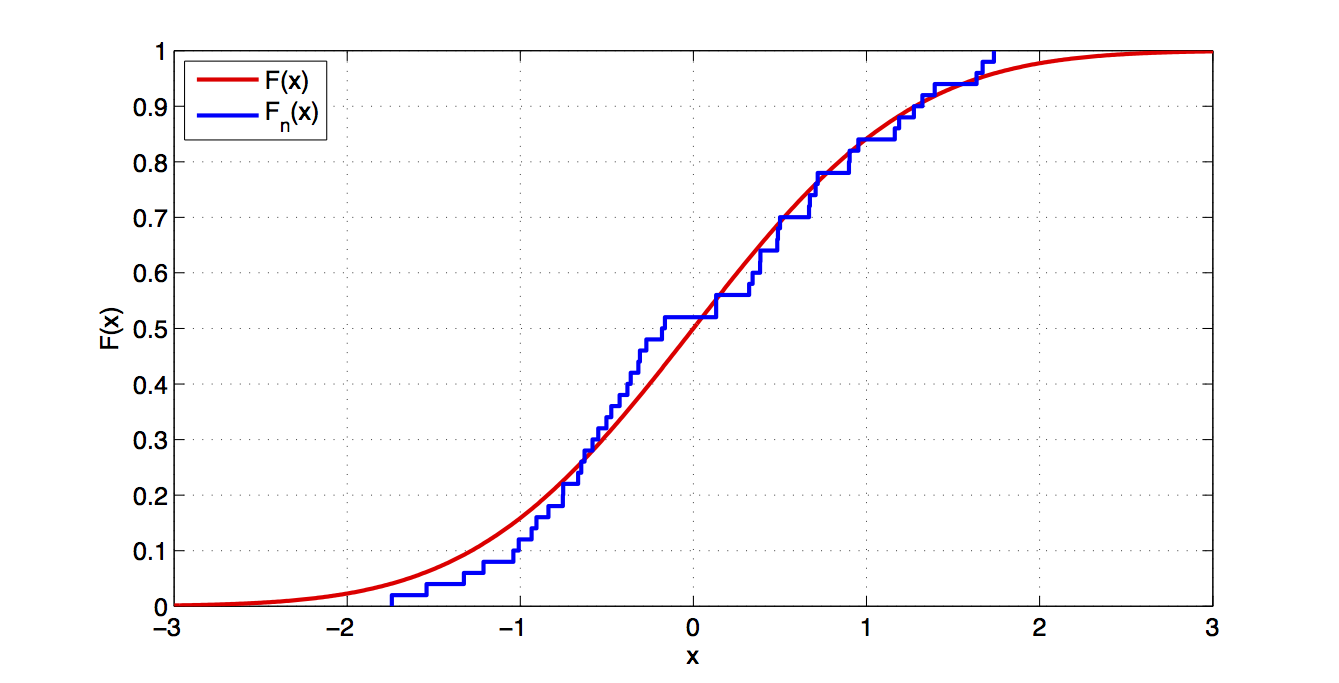
\includegraphics[width=0.9\textwidth]{ecdf.png}
    \end{center}
\end{frame}

\begin{frame}{Эмпирическая функция плотности распределения}
    \begin{center}
        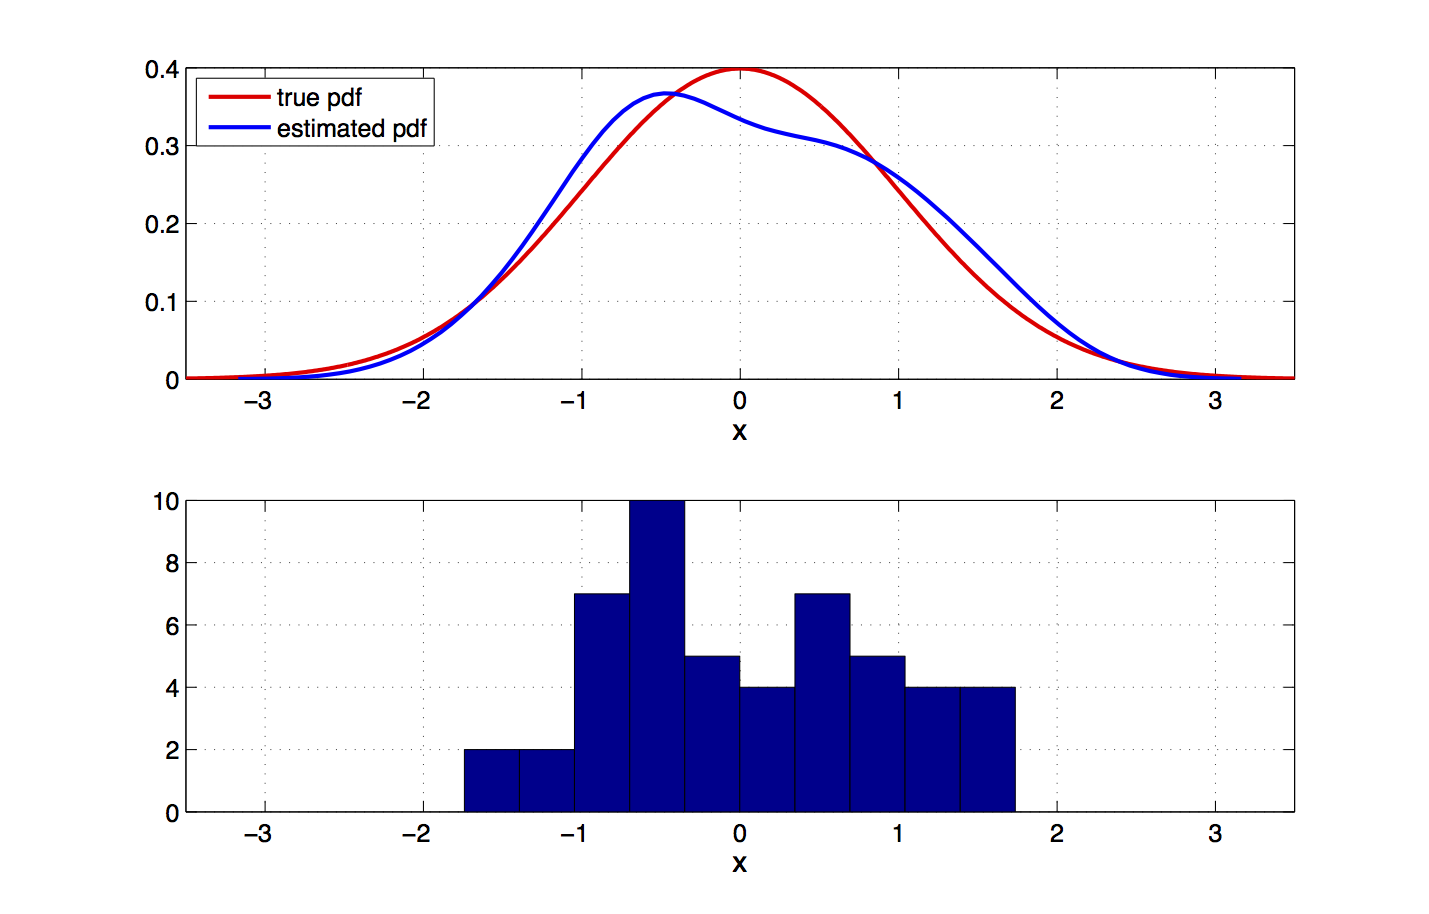
\includegraphics[width=0.8\textwidth]{epdf.png}
    \end{center}


\end{frame}


\begin{frame}{Статистики}
%%%%%%%%%%%%%%%%%%%%%%%%%%%%%%%%%%%%%%%%%%%%%%%%%%%%%%%%%%%%%%%%%%%%%%%
% Мы научились оценивать распределение случайной величины по выборке, можно расходиться! На самом деле нет. Часто нам интересно не распределение целиком, а какие-то его конкретные характеристики. Самые популярные, естественно, средние. Для оценки таких характеристик мы будем использовать основной инструмент статистики - статистики. Слово "измеримая" в курсе больше не будет встречаться никогда.
%%%%%%%%%%%%%%%%%%%%%%%%%%%%%%%%%%%%%%%%%%%%%%%%%%%%%%%%%%%%%%%%%%%%%%%
	\textbf{Статистика} $T(X^n)$~--- любая измеримая функция выборки.

    \structure{Примеры:}
	\begin{itemize}
		\item выборочное среднее:
		$$\bar{X} = \frac{1}{n}\sum\limits_{i=1}^n X_i$$
		\item выборочная дисперсия:
		$$
            S^2 = \frac{1}{n}\sum\limits_{i=1}^n \left(X_i-\bar{X}\right)^2
            \text{ или }
            \hat{S}^2 = \frac{1}{n-1}\sum\limits_{i=1}^n \left(X_i-\bar{X}\right)^2
        $$
	    \item $k$-я порядковая статистика: $X_{(k)}$
		\item выборочный $\alpha$-квантиль: $X_{(\lfloor n\alpha\rfloor)}$
		\item выборочная медиана:
		$
        m = \begin{cases}
		  X_{(k+1)}, & \text{если } n=2k+1, \\
		  \frac{X_{(k)}+X_{(k+1)}}{2}, & \text{если } n=2k.\\
		\end{cases}
        $
	\end{itemize}

%	\only<2>{
%	\begin{itemize}
%		\item выборочный интерквартильный размах:
%			$$IQR_n = X_{([0.75 n])} - X_{([0.25n])}$$
%		\item выборочный коэффициент ассиметрии:
%			$$g_1 = \frac{\sqrt{n} \sum\limits_{i=1}^n \left(X_i-\bar{X}\right)^3}{\left(\sum\limits_{i=1}^n \left(X_i - \bar{X}\right)^2 \right)^{3/2}}$$
%		\item выборочный коэффициент эксцесса:
%		 	$$g_2 = \frac{n \sum\limits_{i=1}^n \left(X_i-\bar{X}\right)^4}{\left(\sum\limits_{i=1}^n \left(X_i - \bar{X}\right)^2 \right)^{2}} -3$$
%	\end{itemize}
%	}
\end{frame}

\subsection{Об ограниченности статистик}
\begin{frame}{Оценки центральной тенденции}{(Huff, 1954)}
%%%%%%%%%%%%%%%%%%%%%%%%%%%%%%%%%%%%%%%%%%%%%%%%%%%%%%%%%%%%%%%%%%%%%%%
% Оценки разных средних, как и сами эти разные средние, вовсе не обязаны совпадать, как, например, у бимодального распределения на картинке. Этим можно пользоваться.
%%%%%%%%%%%%%%%%%%%%%%%%%%%%%%%%%%%%%%%%%%%%%%%%%%%%%%%%%%%%%%%%%%%%%%%
    \begin{multicols}{2}
    \begin{itemize}
        \item Выборочное среднее~--- среднее арифметическое по выборке.
        \item Выборочная медиана~--- центральный элемент вариационного ряда.
        \item Выборочная мода~--- самое распространённое значение в выборке.
    \end{itemize}
    \columnbreak
%     \structure{25 сотрудников:} \hfill (Huff, 1954): \par
    %%%%%%%%%%%%%%%%%%%%%%%%%%%%%%%%%%%%%%%%%%%%%%%%%%%%%%%%%%%%%%%%%%%%%%%
    % Перед вами пример из книги 1954 года "Как врать с помощью статистики". Дана выборка из 25 человек, про которых мы знаем их годовой доход. Представьте, что на основе этих данных нам нужно написать отчёт об уровне дохода в нашей генеральной совокупности, например, стране. Если мы хотим, чтобы отчёт выглядел оптимистично, мы можем написать, что что средний доход составляет $5700. Если нам нужны более пессимистичные оценки, мы можем написать, что большая часть людей получает $2000; ну и промежуточный вариант со средним доходом $3000. Все эти оценки являются оценками разных средних, и часто упоминание того, какое именно среднее было использовано, из текста выбрасывается. Мы рассказываем вам это не для того, чтобы вы так делали~--- за это вы будете гореть в аду~--- а чтобы вы понимали, что другие люди могут так делать.
    %%%%%%%%%%%%%%%%%%%%%%%%%%%%%%%%%%%%%%%%%%%%%%%%%%%%%%%%%%%%%%%%%%%%%%%
    \begin{center}
        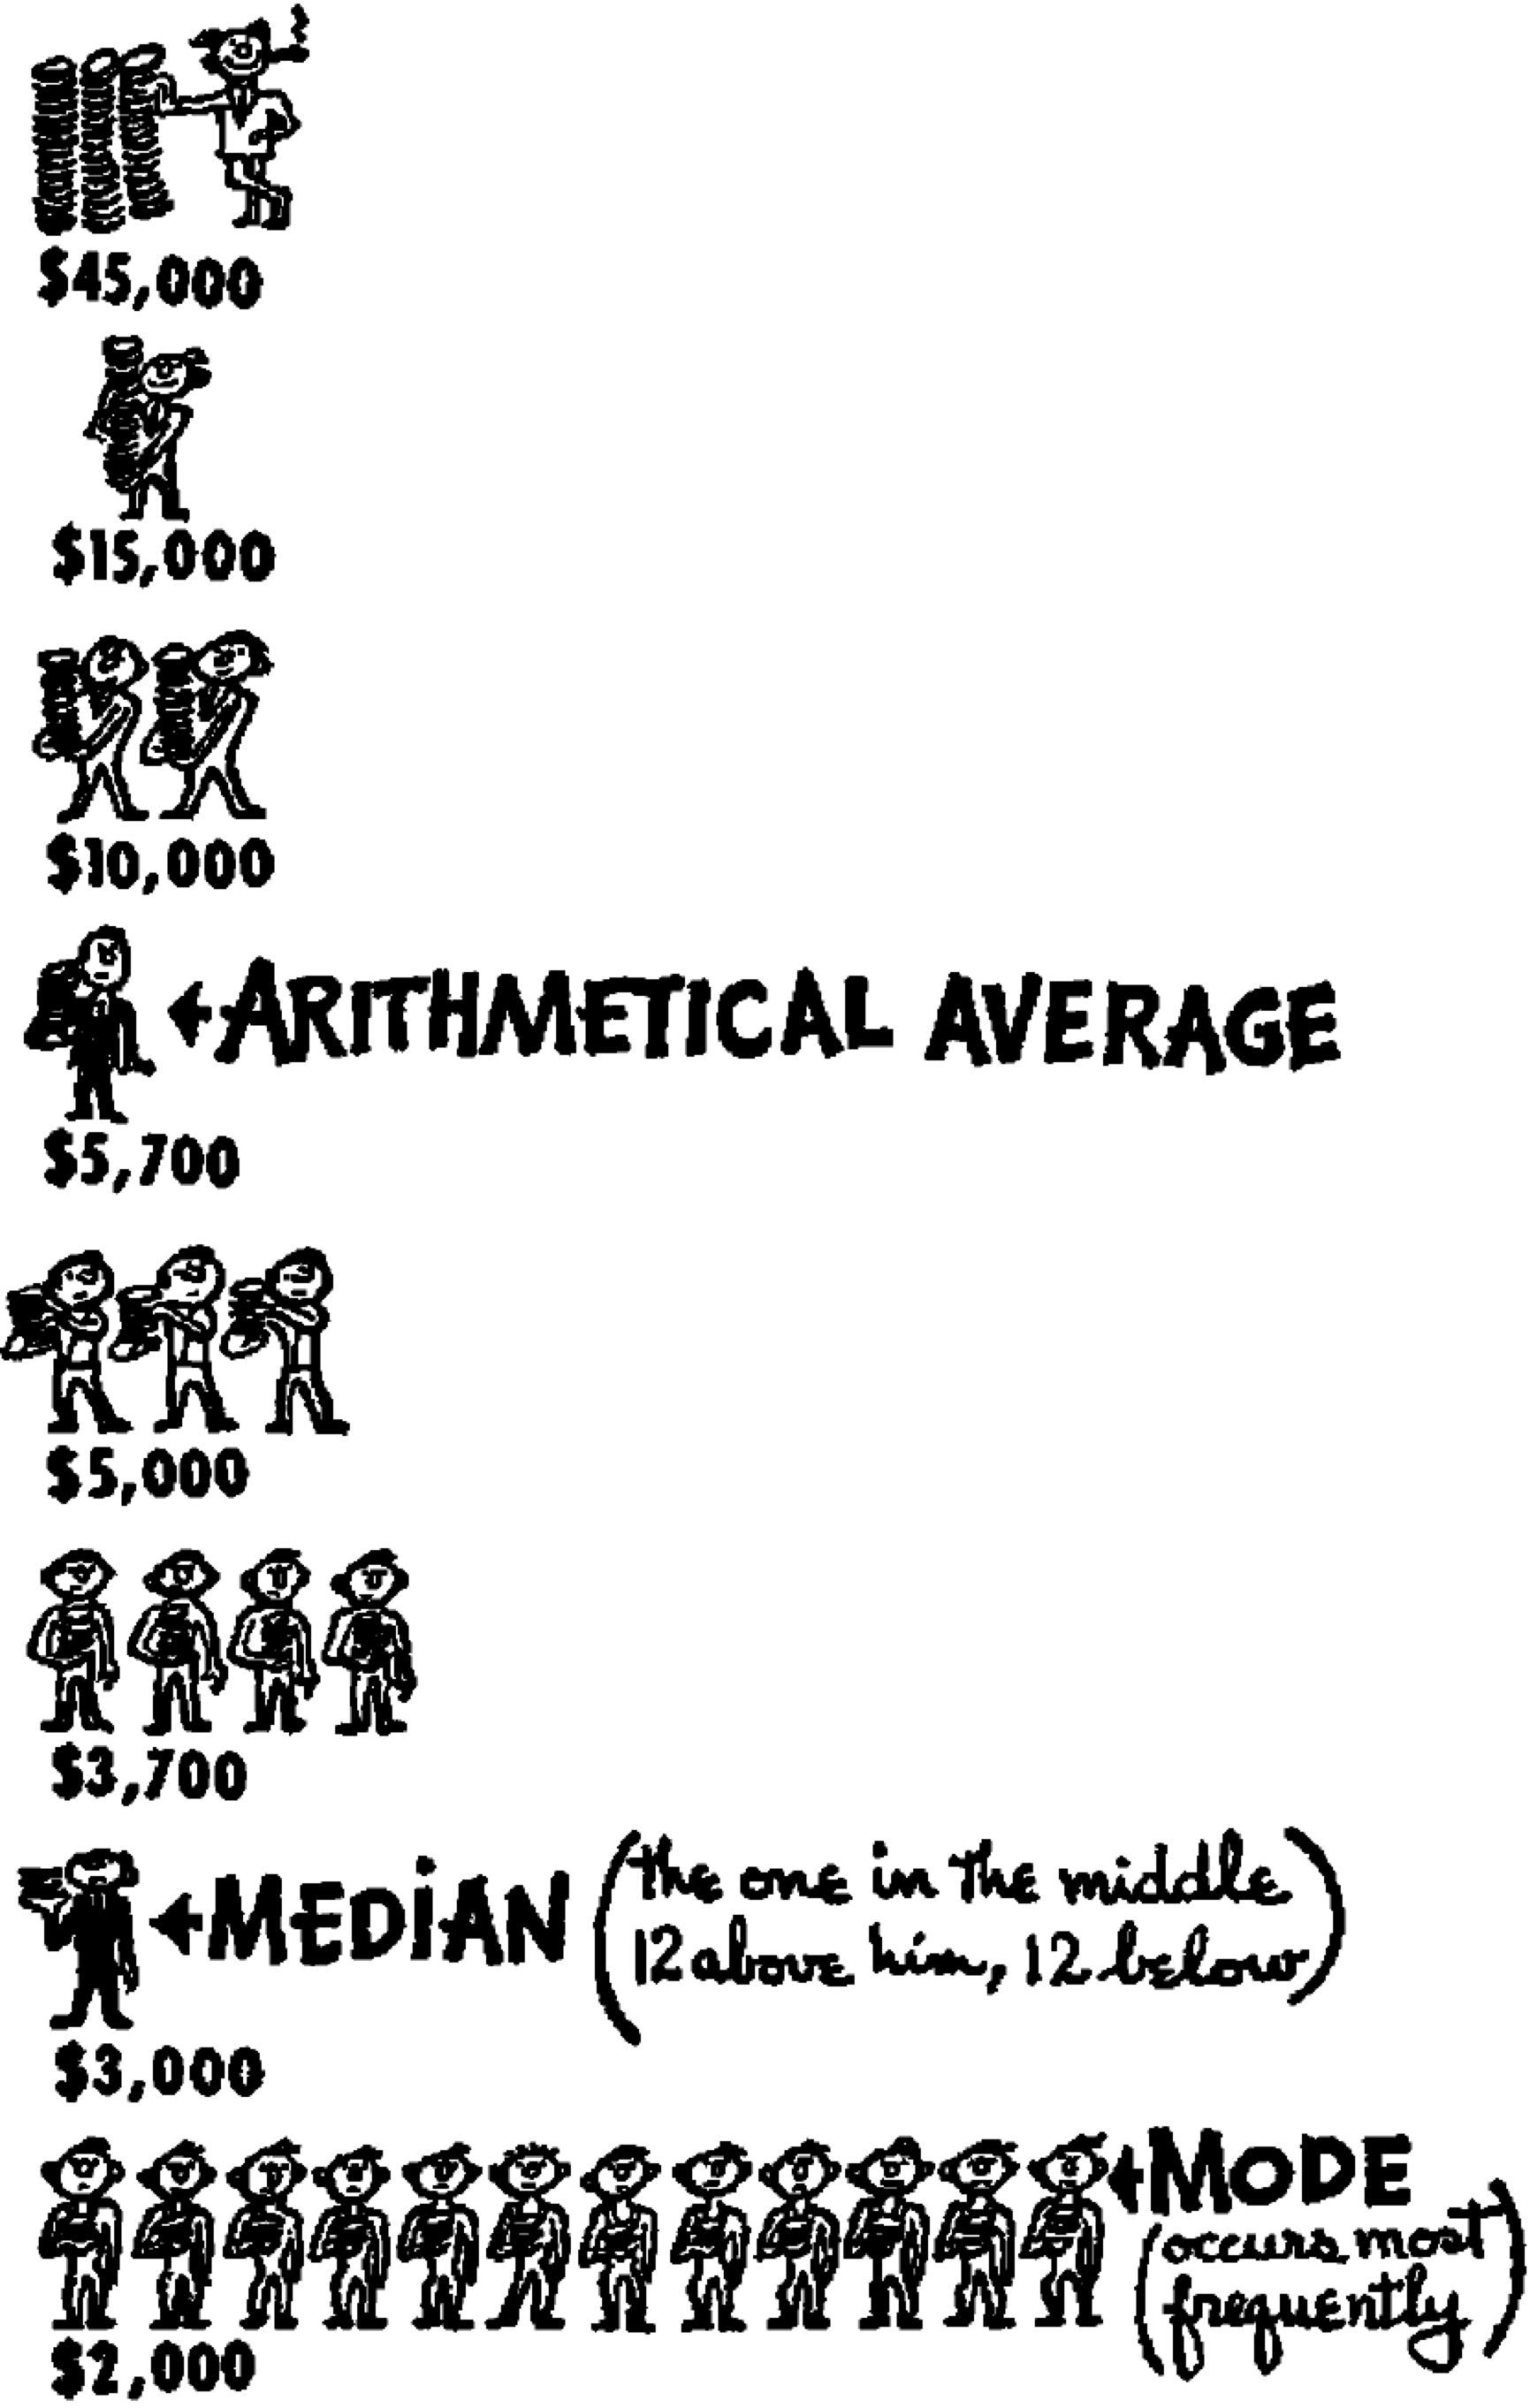
\includegraphics[height=0.85\textheight]{howto.png}
    \end{center}
    \end{multicols}
%    \begin{center}
%        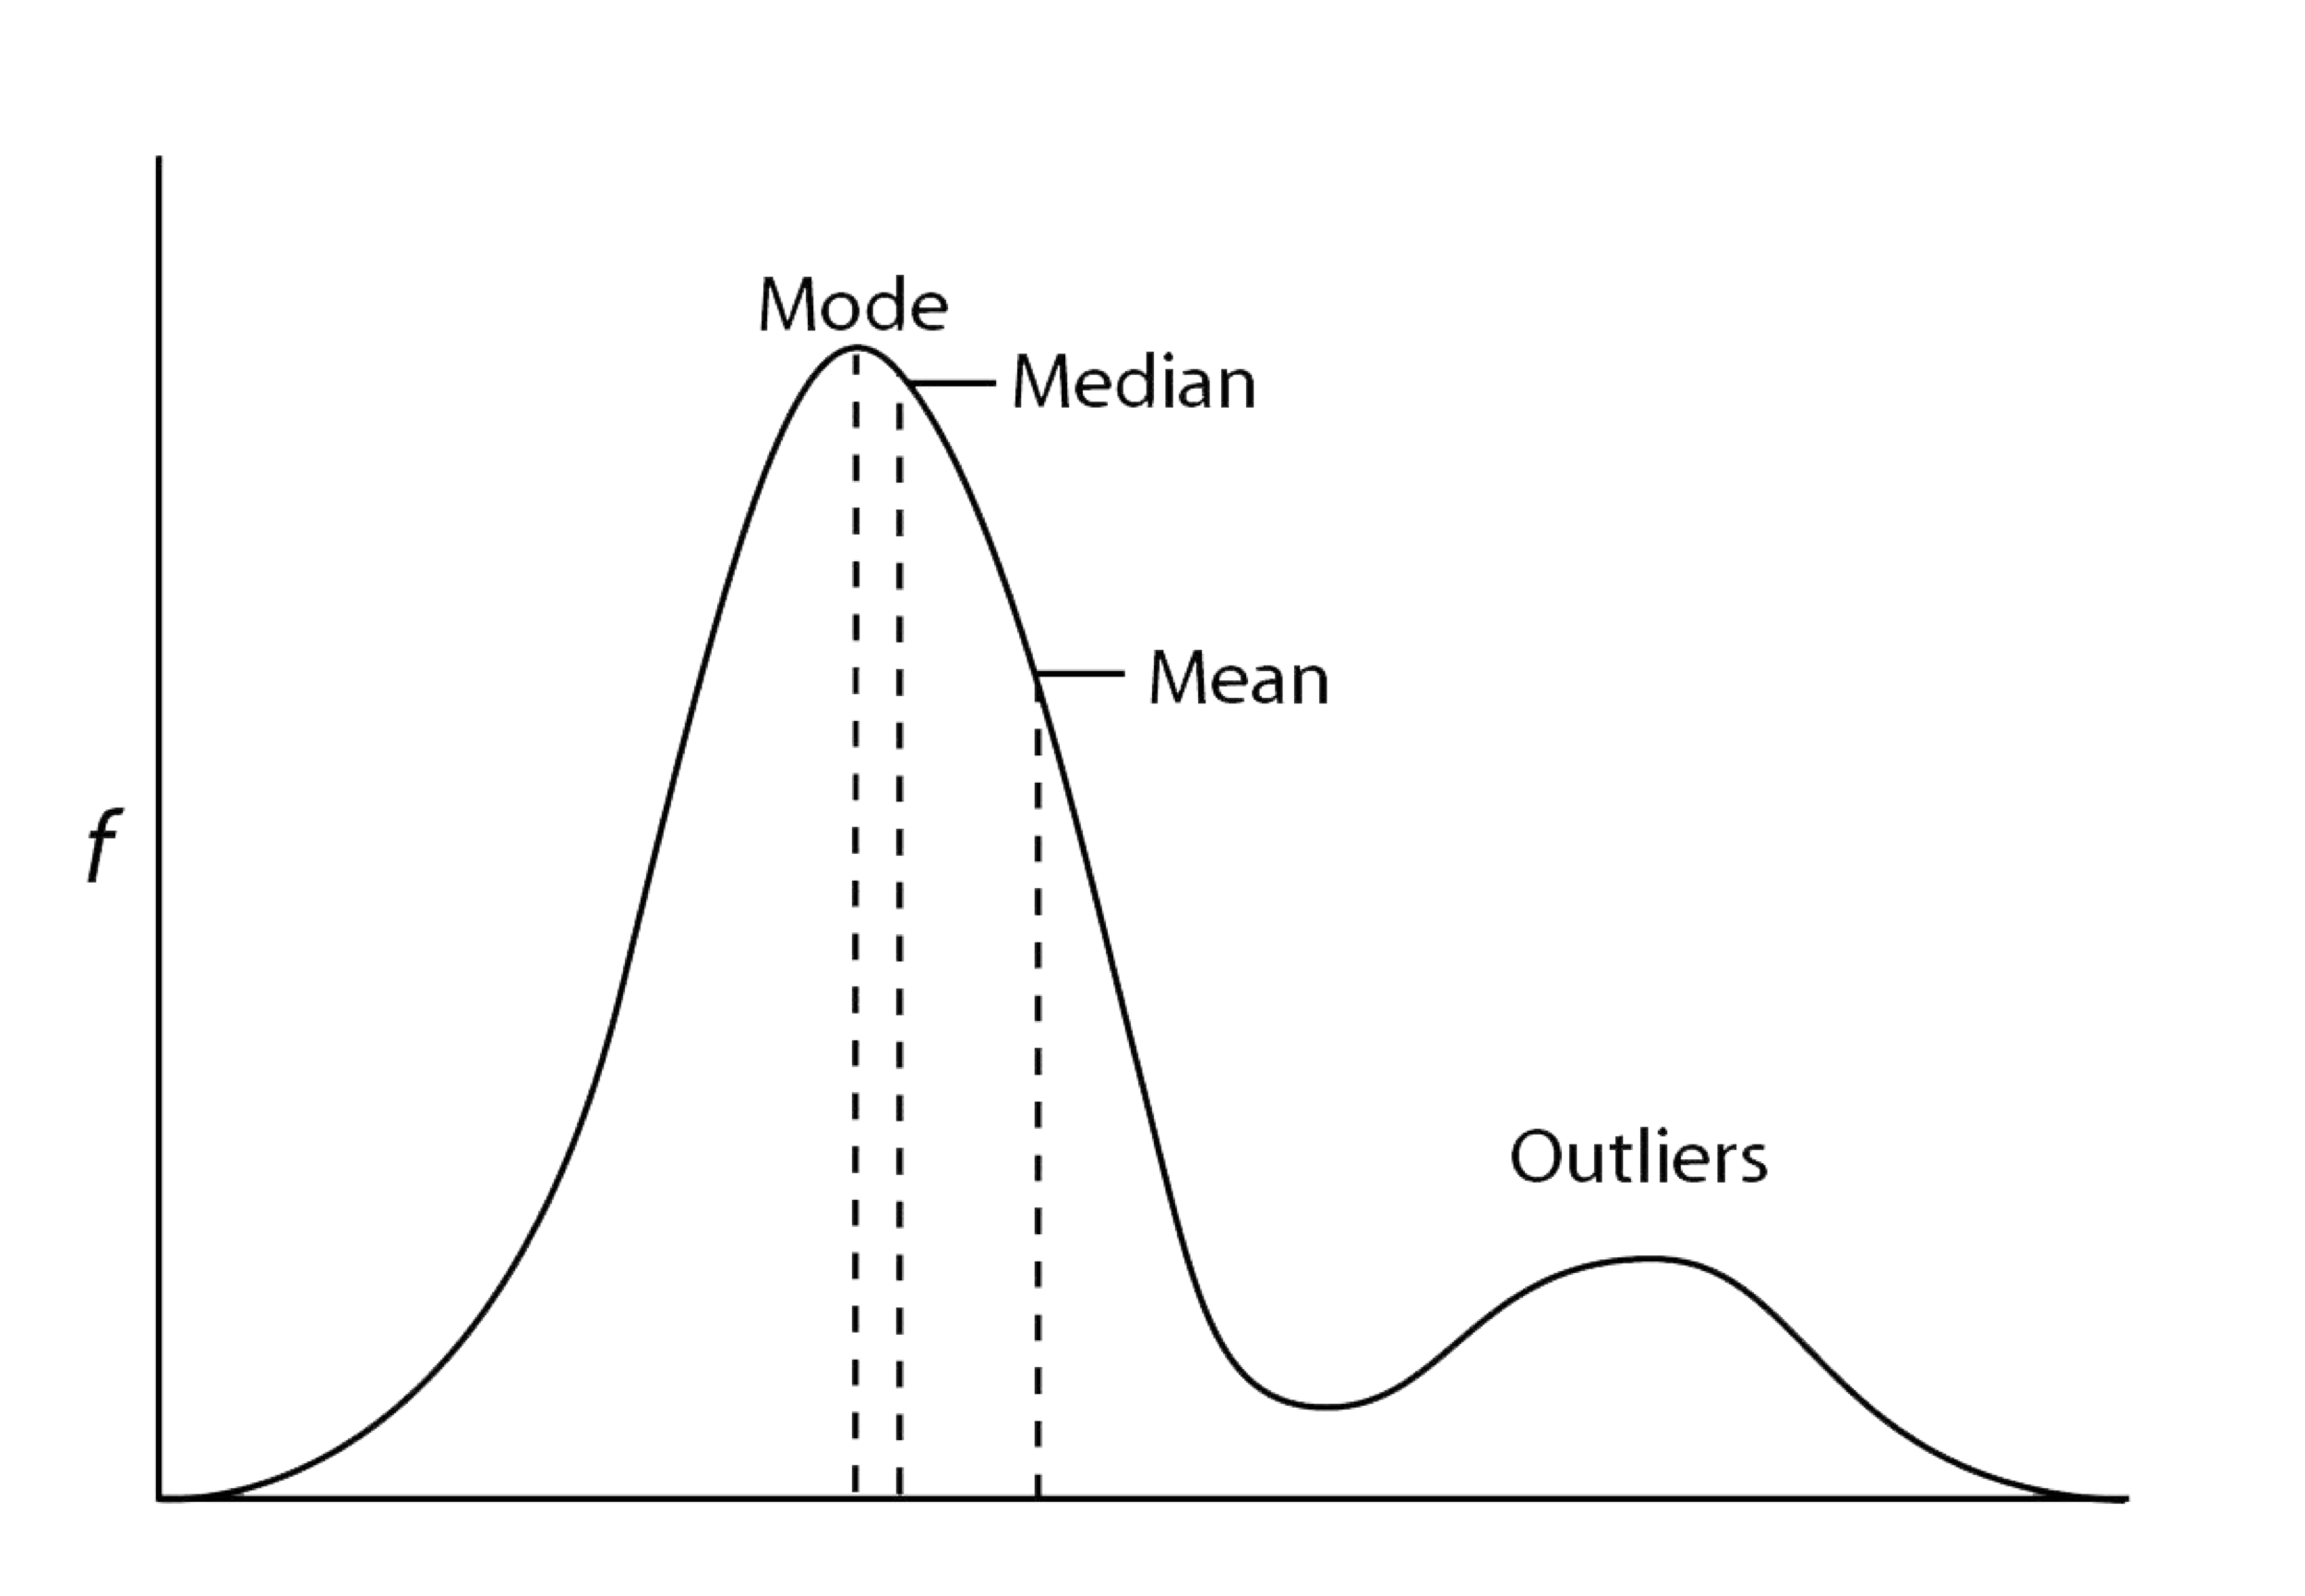
\includegraphics[width=0.5\textwidth]{mmm.png}
%    \end{center}

\end{frame}

\begin{frame}{Мультимодальные распределения}
%%%%%%%%%%%%%%%%%%%%%%%%%%%%%%%%%%%%%%%%%%%%%%%%%%%%%%%%%%%%%%%%%%%%%%%
% Вообще говоря, никакое среднее не может полностью передать распределение исследуемой вами величины. Пример - стартовые заработные платы выпускников юридических факультетов по данным опроса участников американской ассоциации юристов. Их средняя зарплата составляет $80000, но по картинке, которая представляет собой по сути выборочную оценку плотности распределения показателя, хорошо видно, что $80000 не получает примерно никто. Как бы вы не посчитали по этим данным среднее, глядя на него, а не на картинку, вы никогда не поймёте, как устроены ваши данные.
%%%%%%%%%%%%%%%%%%%%%%%%%%%%%%%%%%%%%%%%%%%%%%%%%%%%%%%%%%%%%%%%%%%%%%%
		\begin{center}
			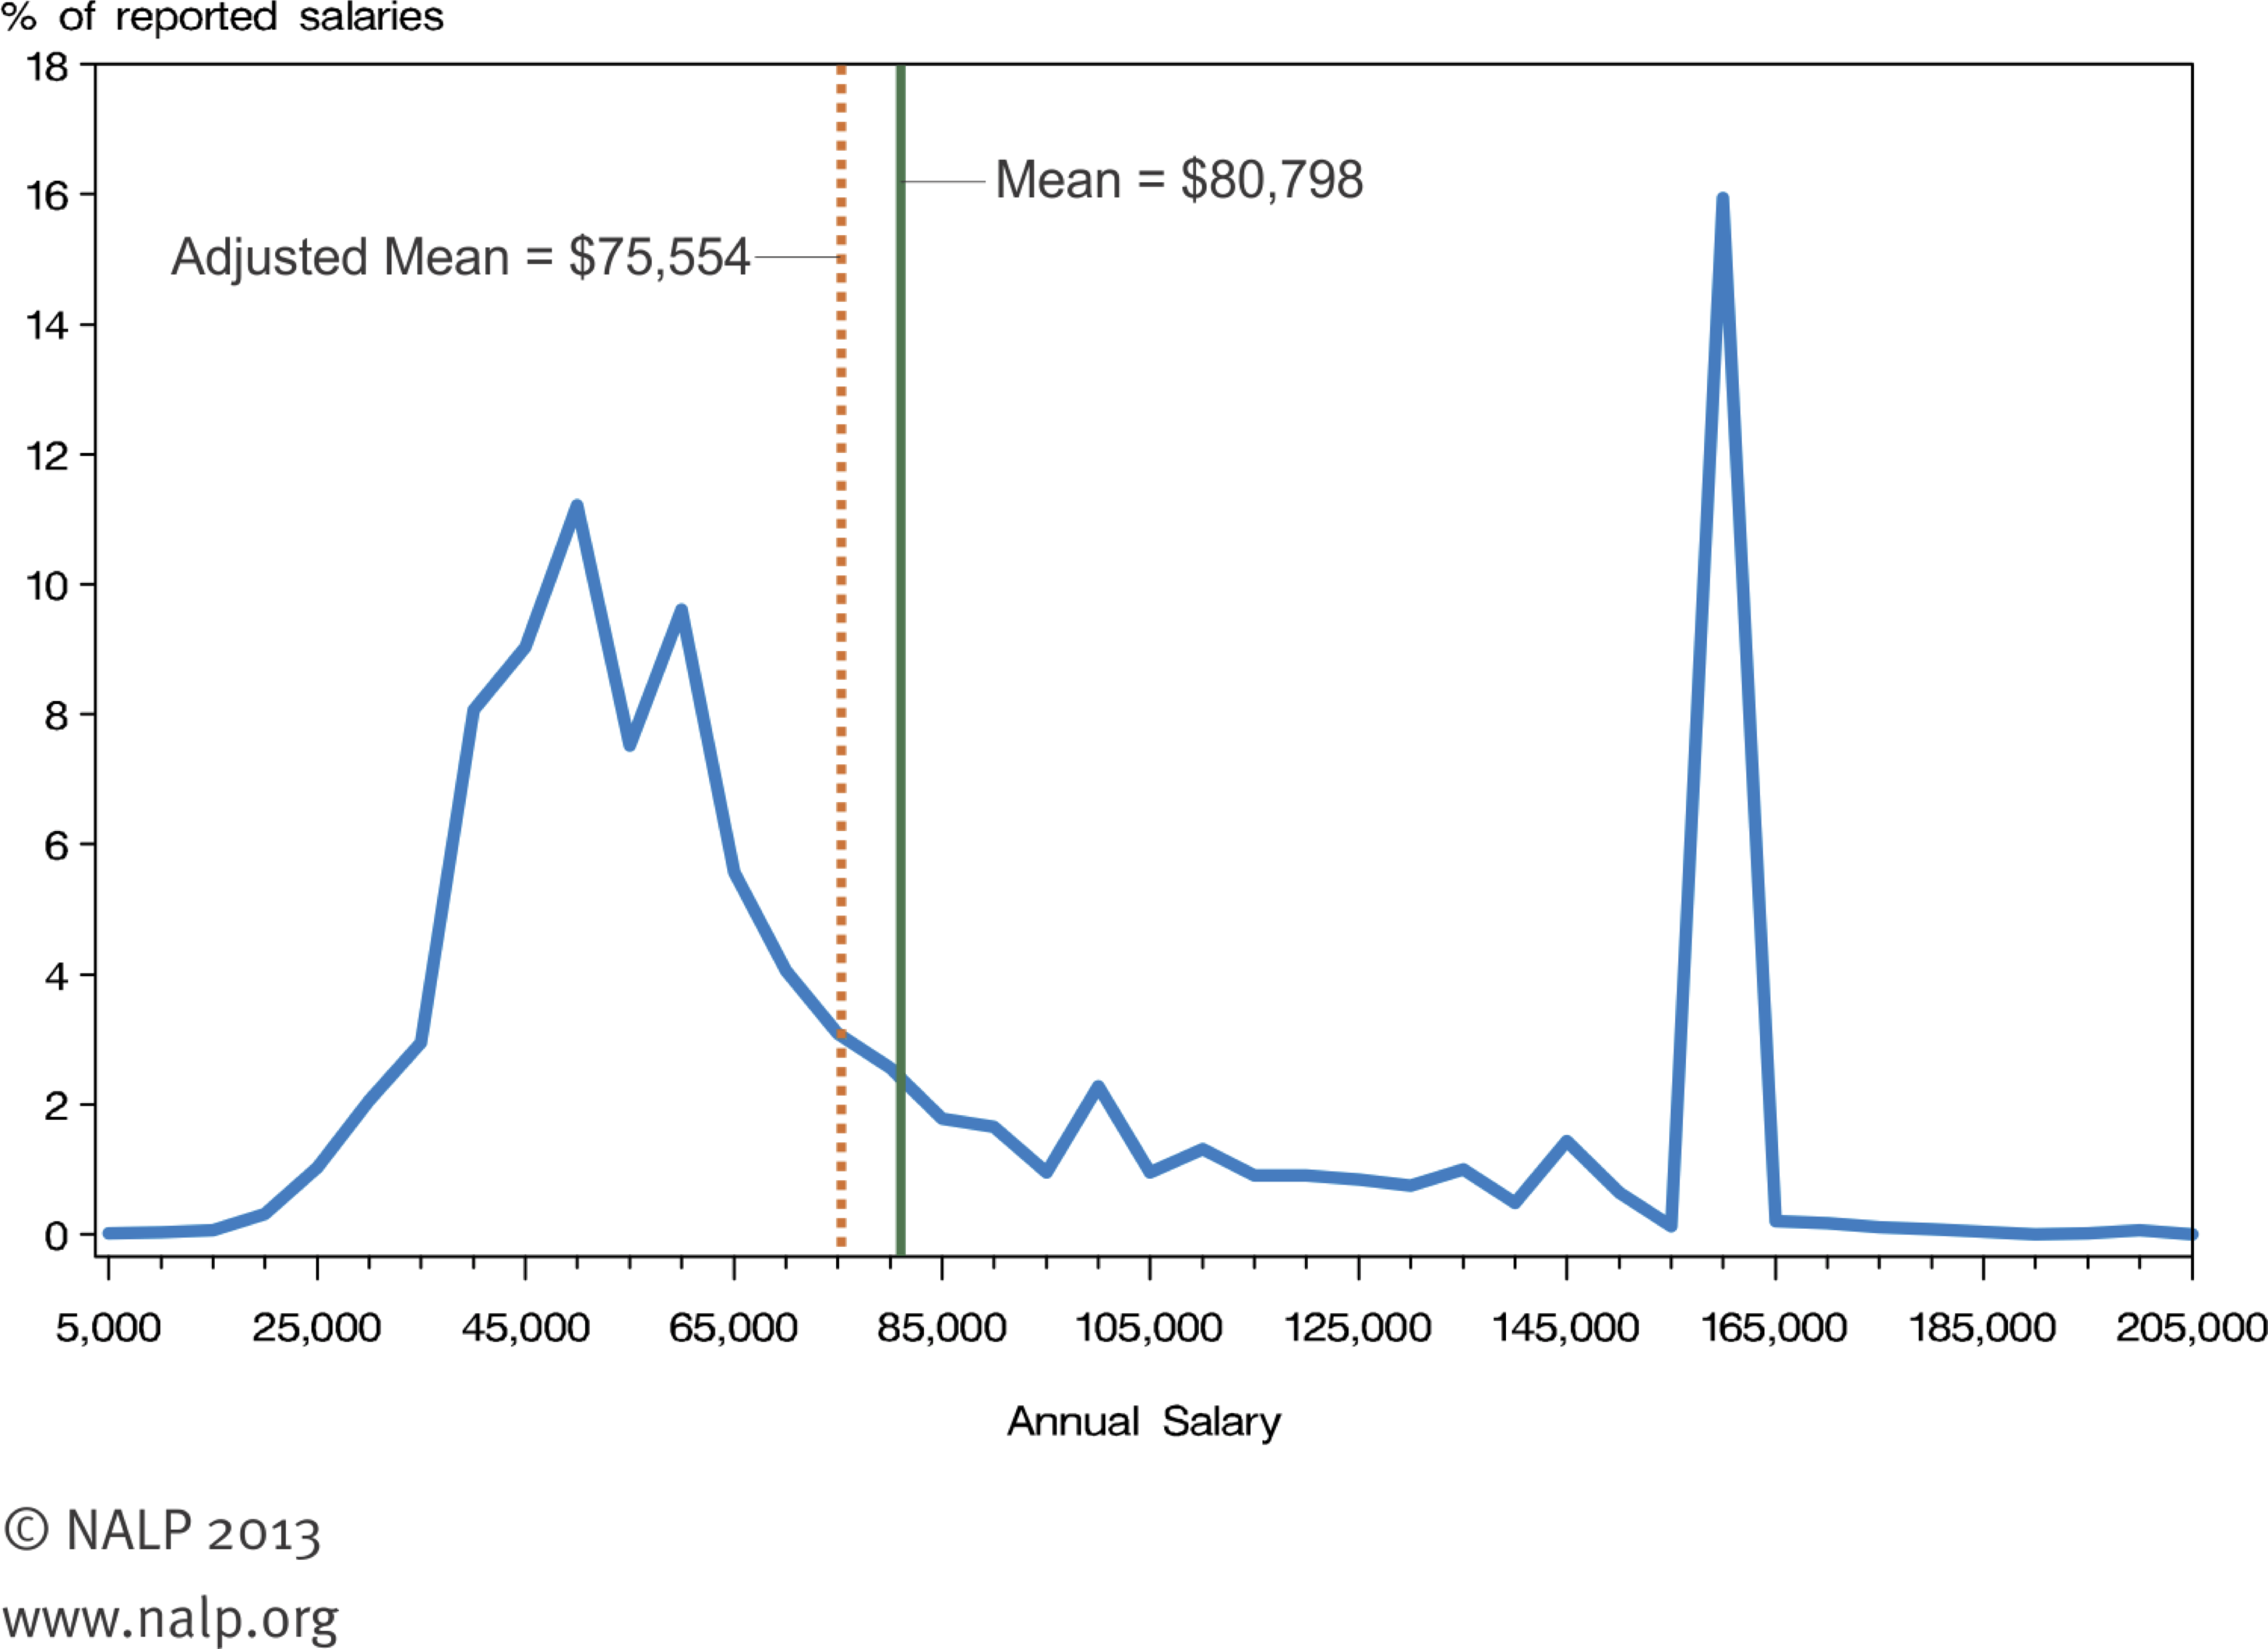
\includegraphics[height=0.7\textheight]{nalp2012.png}
		\end{center}
		Уровень стартовой заработной платы выпускников юридических факультетов, США, 2012
\end{frame}

\begin{frame}{Квартет Энскомба}{(Anscombe, 1973)}

    \begin{multicols}{2}
    \begin{center}
        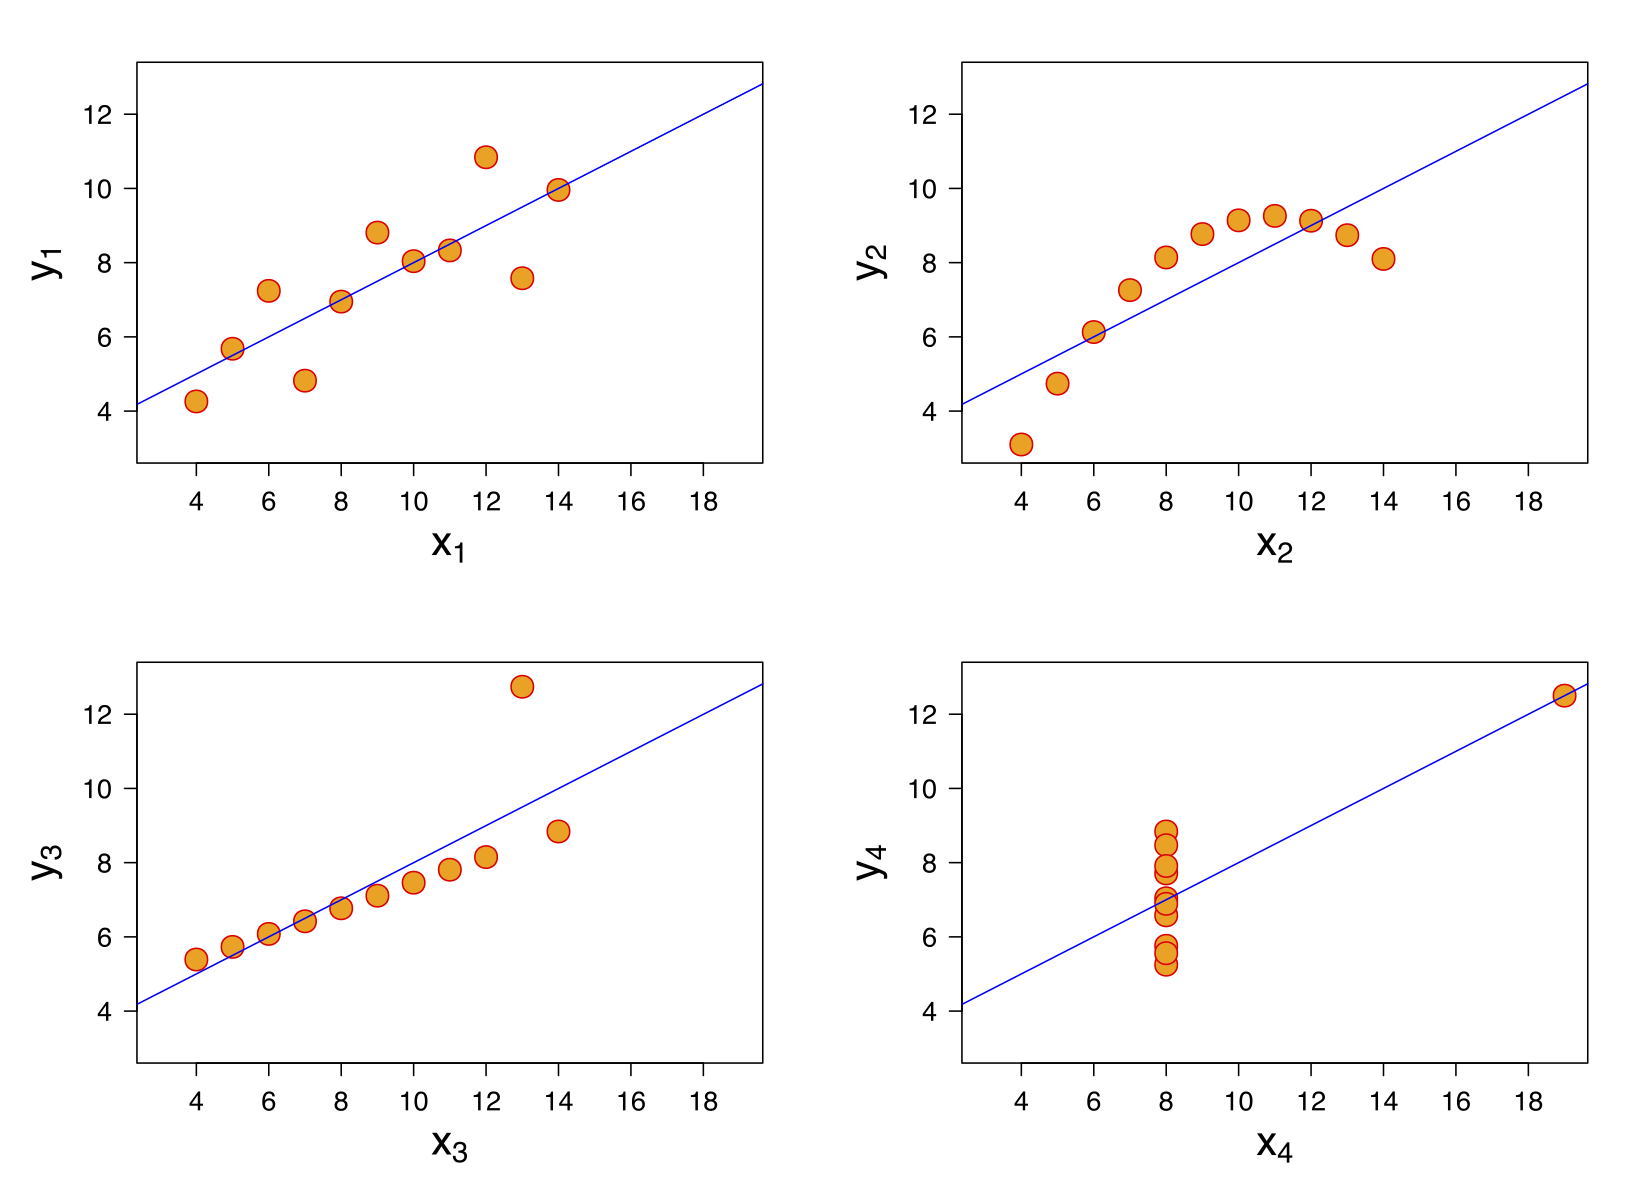
\includegraphics[width=0.55\textwidth]{Anscombe's_quartet.png}
    \end{center}
    \columnbreak
    ~

    \vspace{1cm}
    %%%%%%%%%%%%%%%%%%%%%%%%%%%%%%%%%%%%%%%%%%%%%%%%%%%%%%%%%%%%%%%%%%%%%%%
    % Это справедливо, разумеется, не только для средних. Один из самых известных примеров - это квартет Энскомба, четыре пары таких выборок, что их выборочные средние, дисперсии и корреляции совпадают с точностью до двух знаков после запятой. Таблица показывает нам, что все четыре пары выборок примерно одинаковые,
    %%%%%%%%%%%%%%%%%%%%%%%%%%%%%%%%%%%%%%%%%%%%%%%%%%%%%%%%%%%%%%%%%%%%%%%

		\begin{center}
            \small
			\begin{tabular}{|l|cccc|}
				\hline
				№ & $X_1$    & $X_2$    & $X_3$    & $X_4$ \\ \hline
				$\bar{x}$ & 9    & 9    & 9    & 9    \\ \hline
				$S_x$   & 11   & 11   & 11   & 11   \\ \hline
				$\bar{y}$ & 7.5  & 7.5  & 7.5  & 7.5  \\ \hline
				$S_y$    & 4.127& 4.127& 4.128& 4.128\\ \hline
				$r_{xy}$  & 0.816& 0.816& 0.816& 0.816\\ \hline
			\end{tabular}
		\end{center}
    \end{multicols}
%%%%%%%%%%%%%%%%%%%%%%%%%%%%%%%%%%%%%%%%%%%%%%%%%%%%%%%%%%%%%%%%%%%%%%%
% но, если мы посмотрим, как они выглядят на графиках, мы увидим, что это далеко не так.
% Мораль: не полагайтесь на обобщающие статистики, всегда смотрите на оценки плотности и гистограммы, чтобы понять, как именно ваши данные устроены.
%%%%%%%%%%%%%%%%%%%%%%%%%%%%%%%%%%%%%%%%%%%%%%%%%%%%%%%%%%%%%%%%%%%%%%%
\end{frame}

\section{Оценки}
\subsection{Точечные оценки параметров}
\begin{frame}{}{}
    {\centering
    \bfseries
    \huge Точечные оценки параметров распределения
    \par}
    \bigskip
     Пусть распределение генеральной совокупности параметрическое:
      $$F(x) = F(x,\theta).$$

    Статистика $\hat{\theta}_n = \hat{\theta}\left(X^n\right)$~--- \structure{точечная оценка параметра $\theta$}.

\end{frame}
\begin{frame}{Точечные оценки}
%%%%%%%%%%%%%%%%%%%%%%%%%%%%%%%%%%%%%%%%%%%%%%%%%%%%%%%%%%%%%%%%%%%%%%%
% Определение робастности не строгое, потому что "отклонение" и "выброс" тоже строго не определяются.
%%%%%%%%%%%%%%%%%%%%%%%%%%%%%%%%%%%%%%%%%%%%%%%%%%%%%%%%%%%%%%%%%%%%%%%



    \bigskip

    \section{Свойства точечных оценок:}
    \begin{itemize}
    \item \textbf{Состоятельность:} $\lim\limits_{n\to\infty} \hat{\theta}_n  = \theta$.

    \item \textbf{Несмещённость:} $\EE(\hat{\theta}_n) = \theta$.

    \item \textbf{Асимптотическая несмещённость:} $\lim\limits_{n\to\infty}\EE\hat{\theta}_n = \theta$.

    \item \textbf{Оптимальность:} $\DD(\hat{\theta}_n) = \min\limits_{\hat{\theta}\colon \EE(\hat{\theta})=\theta } \DD(\hat{\theta})$.

    \item \textbf{Робастность:} устойчивость $\hat{\theta}_n$ относительно
    \begin{itemize}
    	\item отклонений истинного распределения~$X$ от модельного семейства
    	\item выбросов, содержащихся в выборке
    \end{itemize}
    \end{itemize}
\end{frame}

\begin{frame}[allowframebreaks]{Метод максимума правдоподобия}{Maximum likelihood estimation (MLE)}
%%%%%%%%%%%%%%%%%%%%%%%%%%%%%%%%%%%%%%%%%%%%%%%%%%%%%%%%%%%%%%%%%%%%%%%
% ММП - популярный метод получения оценок, когда семейства распределений заданы с точностью до параметров.
%%%%%%%%%%%%%%%%%%%%%%%%%%%%%%%%%%%%%%%%%%
	\begin{align*}
	X  &\sim f\left(x, \theta\right), \\
	X^n&=\left(X_1,\dots,X_n\right),
    \end{align*}
  \structure{Цель:} максимизировать вероятность появления имеющейся выборки, меняя параметр~$\theta$.
	\begin{align*}
	L\left(X^n,\theta\right) &= \prod\limits_{i=1}^n f\left(X_i, \theta\right), \\
	\hat{\theta}_{MLE} &= \argmax{\theta} L\left( X^n, \theta \right).
	\end{align*}
	Прологарифмируем:
	\begin{align*}
	\ln L\left(X^n,\theta\right) &= \sum\limits_{i=1}^n f\left(X_i, \theta\right), \\
	\hat{\theta}_{MLE} &= \argmax{\theta} \ln L\left( X^n, \theta \right).
	\end{align*}


	Дифференцируем:
	$$
        S\left(\theta\right) \equiv \frac{\partial}{\partial \theta} \ln L\left(X^N, \theta\right) =
        \sum_{i=1}^n \frac{\partial \ln f(X_i,\theta)}{\partial\theta}
    $$

    Оценка максимального правдоподобия~--- решение уравнения:
	$$S\left(\theta\right)=0$$
\end{frame}
\begin{frame}[allowframebreaks]{Метод максимума правдоподобия}{Пример}
    $$
        X \sim N(\mu,\sigma), \qquad
        N(\mu, \sigma^2) = \frac{1}{\sqrt{2 \pi \sigma^2}} \cdot e^{-\frac{(x - \mu)^2}{2\sigma^2}}
    $$
    $$
        L(\mu, \sigma^2)
        = \prod_{i=1}^n\frac{1}{\sqrt{2\pi \sigma^2}} e^{-\frac{(x_i - \mu)^2}{2\sigma^2}}
        = (2\pi \sigma^2)^{-\frac{n}{2}} e^{-\frac{1}{2\sigma^2} \sum\limits_{i=1}^n(x_i - \mu)^2}
    $$
    $$
        \ln(\mu, \sigma^2) = -\frac{n}{2}\big(\ln(2\pi)+\ln(\sigma^2)\big) - \frac{1}{2\sigma^2}\sum\limits_{i=1}^n(x_i - \mu)^2
    $$
    $$
    \begin{aligned}
        \frac{\partial \ln{L}}{\partial \mu} &= \frac{1}{\sigma^2} \cdot \sum{(x_i - \mu)}\\
        \frac{\partial \ln{L}}{\partial \sigma^2} &= -\frac{n}{2\sigma^2} + \frac{1}{2\sigma^4} \cdot \sum{(x_i - \mu)^2}
    \end{aligned}
    $$
    $$
    \left\lbrace\begin{aligned}
        \frac{1}{\hat\sigma^2} \cdot \sum{(x_i - \hat\mu)} = 0 \\
        -\frac{n}{2\hat\sigma^2} + \frac{1}{2\hat\sigma^4} \cdot \sum{(x_i - \hat\mu)^2} = 0
    \end{aligned}\right.
    \Rightarrow
    \left\lbrace\begin{aligned}
        \sum{(x_i - \hat\mu)} = 0 \\
        -n + \frac{1}{\hat\sigma^2} \cdot \sum{(x_i - \hat\mu)^2} = 0
    \end{aligned}\right.
    $$
    Итак,
    $$
        \alert{\hat\mu = \frac{1}{n}\sum_{i=1}^n{x_i} = \bar{x},}\qquad
        \alert{\hat\sigma^2 = \frac{1}{n} \sum{(x_i - \bar{x})^2=s^2}}
    $$
\end{frame}
\begin{frame}{Информация Фишера}

    Хочется, чтобы функция правдоподобия была выпуклой и очень острой
	\structure{Наблюдаемая информация Фишера}~--- гессиан функции правдоподобия
    $$
        I(\theta) = - \frac{\partial^2\ln{L}}{\partial\theta_i\partial\theta_j}= -H
    $$
    в случае одного параметра:
	$$
        I\left(\theta\right) =  - \frac{\partial^2}{\partial\theta^2}\ln L\left(\theta\right)
    $$

    \bigskip
	\structure{Дисперсия ОМП} (неравенство Рао-Крамера):
	$$\DD\hat{\theta}_{MLE} \geqslant I^{-1}\left(\hat{\theta}_{MLE}\right)$$
\end{frame}

\begin{frame}{Свойства ОМП}
%%%%%%%%%%%%%%%%%%%%%%%%%%%%%%%%%%%%%%%%%%%%%%%%%%%%%%%%%%%%%%%%%%%%%%%
%
%%%%%%%%%%%%%%%%%%%%%%%%%%%%%%%%%%%%%%%%%%%%%%%%%%%%%%%%%%%%%%%%%%%%%%%
	\begin{itemize}
		\item состоятельность: $$\plim\limits_{n\rightarrow\infty} \hat{\theta}_{MLE}  = \theta$$
		\item асимптотическая нормальность: при $n\rightarrow \infty$ $$\hat{\theta}_{MLE}\sim N\left(\theta, I^{-1}(\theta)\right)$$
		\item эффективность: ОМП имеют наименьшую дисперсию среди всех состоятельных оценок
		\item инвариантность: $g\left(\hat{\theta}_{MLE}\right)$~--- ОМП-оценка для $g\left(\theta\right)$
	\end{itemize}

    \medskip
    \hrule

    \medskip

    \slshape
    \small
    О методе максимального правдоподобия можно почитать на Хабре:

    \raggedleft
    \href{https://habr.com/ru/articles/830326/}{Простыми словами о методе максимального правдоподобия и информации Фишера} \url{https://habr.com/ru/articles/830326/}
\end{frame}




\begin{frame}{Несмещенные состоятельные оценки}{}
    \begin{itemize}
        \item Выборочная доля $w = \frac{n(A)}{n}$~--- оценка генеральной доли $\prob(A) = \frac{n_A}{N}$.
            $$
                \sigma_w^2=\frac{pq}{n}\left(\frac{N-n}{N-1}\right),
                \qquad
                \alert{\sigma_w^2= \frac{pq}{n}}
            $$
        \item Выборочная средняя $\bar{x}$~--- оценка генеральной средней $\EE{X}$.
            $$
                \sigma_{\bar{x}}^2=\frac{\sigma^2}{n}\left(\frac{N-n}{N-1}\right),
                \qquad
                \alert{\sigma_{\bar{x}}^2=\frac{\sigma^2}{n}}
            $$
        \item Исправленная выборочная дисперсия $\hat{s}^2$~--- оценка генеральной дисперсии $\DD(X)$.
    \end{itemize}

\end{frame}
\begin{frame}{Интервальные оценки}
%%%%%%%%%%%%%%%%%%%%%%%%%%%%%%%%%%%%%%%%%%%%%%%%%%%%%%%%%%%%%%%%%%%%%%%
%
%%%%%%%%%%%%%%%%%%%%%%%%%%%%%%%%%%%%%%%%%%%%%%%%%%%%%%%%%%%%%%%%%%%%%%%
    \structure{Доверительный интервал:}
    $$
        \prob\left(\theta \in \left[C_L, C_U\right]\right)\geqslant \gamma,
    $$
    \begin{itemize}
    \item $\gamma = 1-\alpha$~--- уровень доверия (\structure{надежность} доверительного интервала),
    \item $C_L$, $C_U$~--- нижний и верхний доверительные пределы.
    \end{itemize}
    \bigskip

	\textbf{Неверная интерпретация}: неизвестный параметр лежит в пределах построенного доверительного интервала с вероятностью $\gamma$.

	\bigskip
    \hrule

    \medskip

    \textbf{Верная интерпретация:} при бесконечном повторении процедуры построения доверительного интервала на аналогичных выборках в~$\gamma\cdot 100\%$ случаев он будет содержать истинное значение~$\theta$.
\end{frame}

\begin{frame}{Оценка среднего для нормального распределения}{параметрический метод}
%%%%%%%%%%%%%%%%%%%%%%%%%%%%%%%%%%%%%%%%%%%%%%%%%%%%%%%%%%%%%%%%%%%%%%%
% по сути это более точная версия правил 2-3 сигм, обобщённая на произвольное количество сигм
%%%%%%%%%%%%%%%%%%%%%%%%%%%%%%%%%%%%%%%%%%%%%%%%%%%%%%%%%%%%%%%%%%%%%%%
	$X\sim N\left(\mu,\sigma^2\right),\;\; X^n=\left(X_1,\dots,X_n\right),$

	\bigskip

	$\bar{X}_n$~--- оценка $\EE{X}=\mu,$
	\bigskip

    $\bar{X}_n\sim N\left(\mu, \frac{\sigma^2}{n}\right) \Rightarrow $
	$$
        \prob \left(
            \mu-z_{1-\frac{\alpha}{2}}\sigma_{\bar{x}}
            \leqslant \bar{X}_n \leqslant
            \mu +z_{1-\frac{\alpha}{2}}\sigma_{\bar{x}}
        \right)
        = 1-\alpha \Longrightarrow
    $$
	доверительный интервал для $\mu$:
	$$
    \alert{\prob \left(
        \bar{X}_n-z_{1-\frac{\alpha}{2}}\sigma_{\bar{x}}
        \leqslant \mu \leqslant
        \bar{X}_n +z_{1-\frac{\alpha}{2}} \sigma_{\bar{x}}
    \right)
    =
    1-\alpha},
    $$
	$z_{1-\frac{\alpha}{2}}$~--- квантиль стандартного нормального распределения $N(0,1)$.

    \structure{Вычисление квантиля:} \texttt{scipy.stats.norm.ppf(1-a/2)}
\end{frame}

\begin{frame}{Оценка среднего для ненормальных распределений}{параметрический метод}
%%%%%%%%%%%%%%%%%%%%%%%%%%%%%%%%%%%%%%%%%%%%%%%%%%%%%%%%%%%%%%%%%%%%%%%
% для ненормальных распределений интервалы приближённые
%%%%%%%%%%%%%%%%%%%%%%%%%%%%%%%%%%%%%%%%%%%%%%%%%%%%%%%%%%%%%%%%%%%%%%%
	\structure{ЦПТ:} \textit{Если $X^n$~--- выборка из $F(x)$, $F(x)$~не~слишком скошено и $n>30$, то
	$$\bar{X}_n \sim N\left(\EE{X}, \frac{\DD{X}}{n}\right).$$}

	доверительный интервал для $\EE{X}$:
	$$\prob \left(\bar{X}_n-z_{1-\frac{\alpha}{2}} \sqrt{\frac{\DD{X}}{n}}
    \leqslant \EE{X} \leqslant \bar{X}_n +z_{1-\frac{\alpha}{2}} \sqrt{\frac{\DD{X}}{n}} \right)\approx 1-\alpha.$$

	Если дисперсия неизвестна:
	$$\alert{\prob \left(
        \bar{X}_n-t_{n-1, 1-\frac{\alpha}{2}} \frac{\hat{s}_n}{\sqrt{n}}
        \leqslant \EE{X} \leqslant
        \bar{X}_n +t_{n-1, 1-\frac{\alpha}{2}} \frac{\hat{s}_n}{\sqrt{n}} \right
        )\approx 1-\alpha,}
    $$
	$t_{n-1, 1-\frac{\alpha}{2}}$~--- квантиль распределения Стьюдента с $n-1$ степенью свободы.

    \structure{Вычисление квантиля:} \texttt{scipy.stats.t.ppf(1-a/2,n-1)}
\end{frame}

\subsection{Непараметрические методы}

\begin{frame}{Интервальная оценка для квантиля произвольного распределения}{непараметрический метод}
%%%%%%%%%%%%%%%%%%%%%%%%%%%%%%%%%%%%%%%%%%%%%%%%%%%%%%%%%%%%%%%%%%%%%%%
% На этом слайде мы построили доверительный интервал для квантиля произвольного непрерывного распределения, не ограничивая класс распределений параметрическими предположениями. Далее мы рассмотрим ещё один непараметрический способ получения оценок.
%%%%%%%%%%%%%%%%%%%%%%%%%%%%%%%%%%%%%%%%%%%%%%%%%%%%%%%%%%%%%%%%%%%%%%%
	Для медианы $X_{0.5}$:
	$$
    X^n = \left(X_1,\dots, X_n\right), \;\; X\sim    F\left(x\right)\; \Longrightarrow
    $$
	   $$\prob\left(\med X \in \left[X_{(r)}, X_{(n-r+1)}\right]\right) =  \sum\limits_{i=r}^{n-r+1} C_n^i\frac{1}{2^n}.
    $$

	При $n>10$ применима нормальная аппроксимация:

	$$
    \alert{\prob\left(\med X \in \left[X_{\left(\left\lfloor \frac{n - \sqrt{n} z_{1-\frac{\alpha}{2}}}{2} \right\rfloor\right)}, X_{\left(\left\lceil  \frac{n + \sqrt{n} z_{1-\frac{\alpha}{2}}}{2} \right\rceil \right)}\right]\right) \approx 1-\alpha.}
    $$

	\bigskip

	Аналогично строится непараметрический доверительный интервал для любого квантиля $X_a$, $a\in\left(0,1\right)$:
	$$
    \alert{\prob\left(X_a \in \left[X_{(l)}, X_{(u)}\right]\right) = \sum\nolimits_{i=l}^u C_n^i a^i \left(1-a\right)^{n-i}.}
    $$
\end{frame}

\subsection{Бутстреп}
\begin{frame}[allowframebreaks]{Построение доверительных интервалов}{to pull oneself up by one's bootstraps}
%%%%%%%%%%%%%%%%%%%%%%%%%%%%%%%%%%%%%%%%%%%%%%%%%%%%%%%%%%%%%%%%%%%%%%%
% Чтобы построить доверительный интервал для параметра, который оценивает наша статистика, нужно понимать, как эта статистика распределена. Есть три способа. Предположить, что распределение признака в генеральной совокупности какое-то параметрическое и вывести из этого предположения закон распределения статистики - работает не всегда: во-первых, не всегда можно предположить, как распределена совокупность, во-вторых, не для всех статистик из этого предположения можно что-то вывести.
%%%%%%%%%%%%%%%%%%%%%%%%%%%%%%%%%%%%%%%%%%%%%%%%%%%%%%%%%%%%%%%%%%%%%%%
		Как можно оценить  $F_{\hat{\theta}_n}\left(x\right)$~--- выборочное распределение статистики $\hat{\theta}_n$?

		(Hesterberg, 2005):

        \structure{Параметрический метод}: 	Сделать предположение, что $X$ распределена по закону~$F_X\left(x\right)$, при выполнении которого закон распределения $\hat{\theta}_n$ известен.
		\begin{figure}
			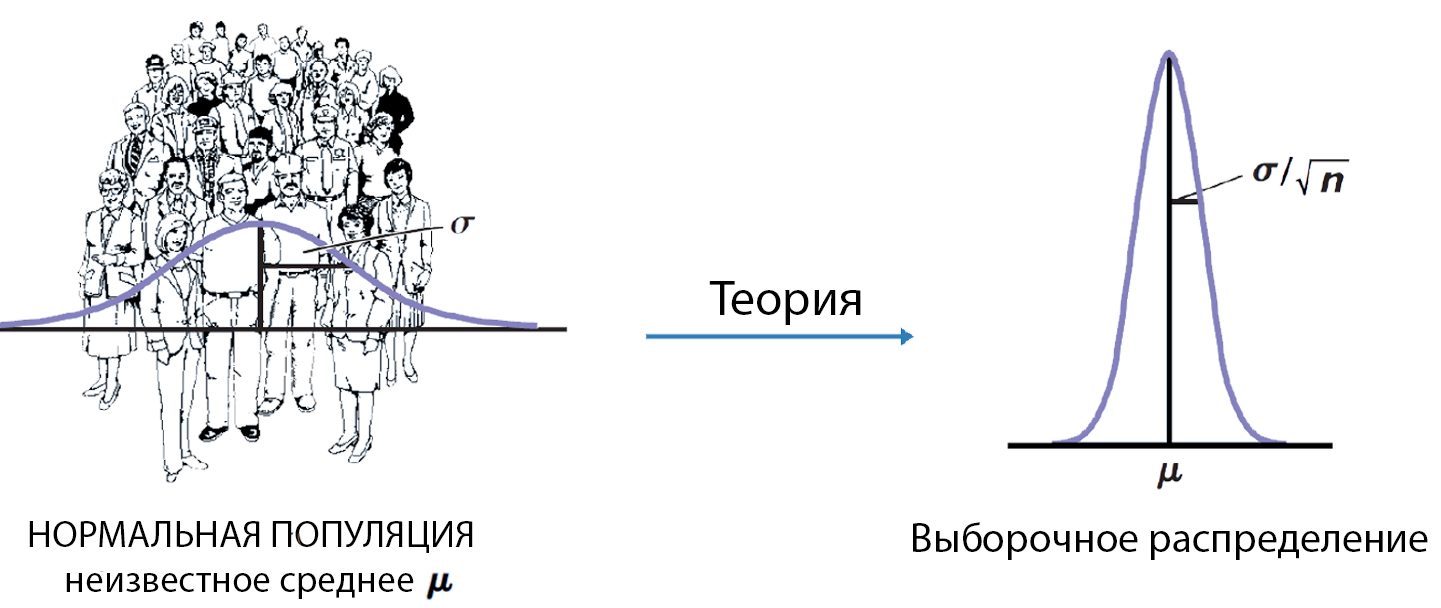
\includegraphics[width=0.7\textwidth]{boot1.png}
		\end{figure}


    \framebreak
%%%%%%%%%%%%%%%%%%%%%%%%%%%%%%%%%%%%%%%%%%%%%%%%%%%%%%%%%%%%%%%%%%%%%%%
% Второй способ - наивный: извлечь из генеральной совокупности много выборок одного и того же размера n, на каждой вычислить значение статистики и по полученной выборке значений оценить её распределение гистограммой или чем-то ещё. Этот метод применим скорее в теории, чем на практике: если не представляет сложности неограниченно генерировать выборки из генеральной совокупности, то можно и саму статистику вычислить на генеральной совокупности, а значит, интервальная оценка не нужна, поскольку известно настоящее значения статистики.
%%%%%%%%%%%%%%%%%%%%%%%%%%%%%%%%%%%%%%%%%%%%%%%%%%%%%%%%%%%%%%%%%%%%%%%

		\structure{Наивный метод:} Извлечь из генеральной совокупности~$N$ выборок объёма~$n$ и оценить выборочное распределение $\hat{\theta}_n$ эмпирическим.

		\begin{figure}
			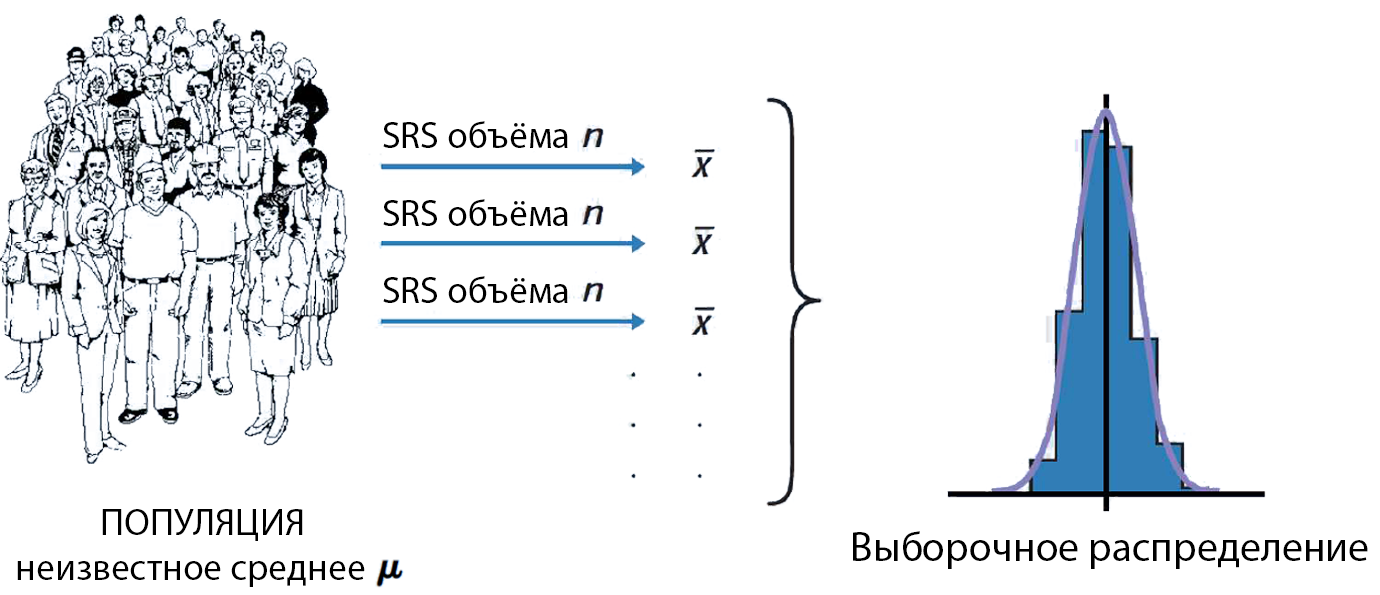
\includegraphics[width=0.8\textwidth]{boot2.png}
		\end{figure}

    \framebreak

%%%%%%%%%%%%%%%%%%%%%%%%%%%%%%%%%%%%%%%%%%%%%%%%%%%%%%%%%%%%%%%%%%%%%%%
% Давайте считать, что мы находимся в реальном мире и доступа к генеральной совокупности у нас нет, а есть только  выборка объёма n. Давайте из этой выборки сделаем много псевдовыборок - выборок с возвращениями - того же самого объёма n. На каждой псевдовыборке посчитаем значение статистики; оказывается, что распределение значений статистики на псевдовыборках часто является хорошей оценкой истинного распределения статистики. Так работает бутстреп (слово означает петлю, которая пришита к заднему краю армейских ботинок, и отсылает нас к выражению "to pull oneself up by one's bootstraps" - что-то вроде Мюнхаузена, вытаскивающего себя из болота за волосы. Действительно, это выглядит как магия.
%%%%%%%%%%%%%%%%%%%%%%%%%%%%%%%%%%%%%%%%%%%%%%%%%%%%%%%%%%%%%%%%%%%%%%%
		\structure{Бутстреп:} Сгенерировать~$N$ <<псевдовыборок>> объёма~$n$ и оценить выборочное распределение $\hat{\theta}_n$ <<псевдоэмпирическим>>.
		\begin{figure}
			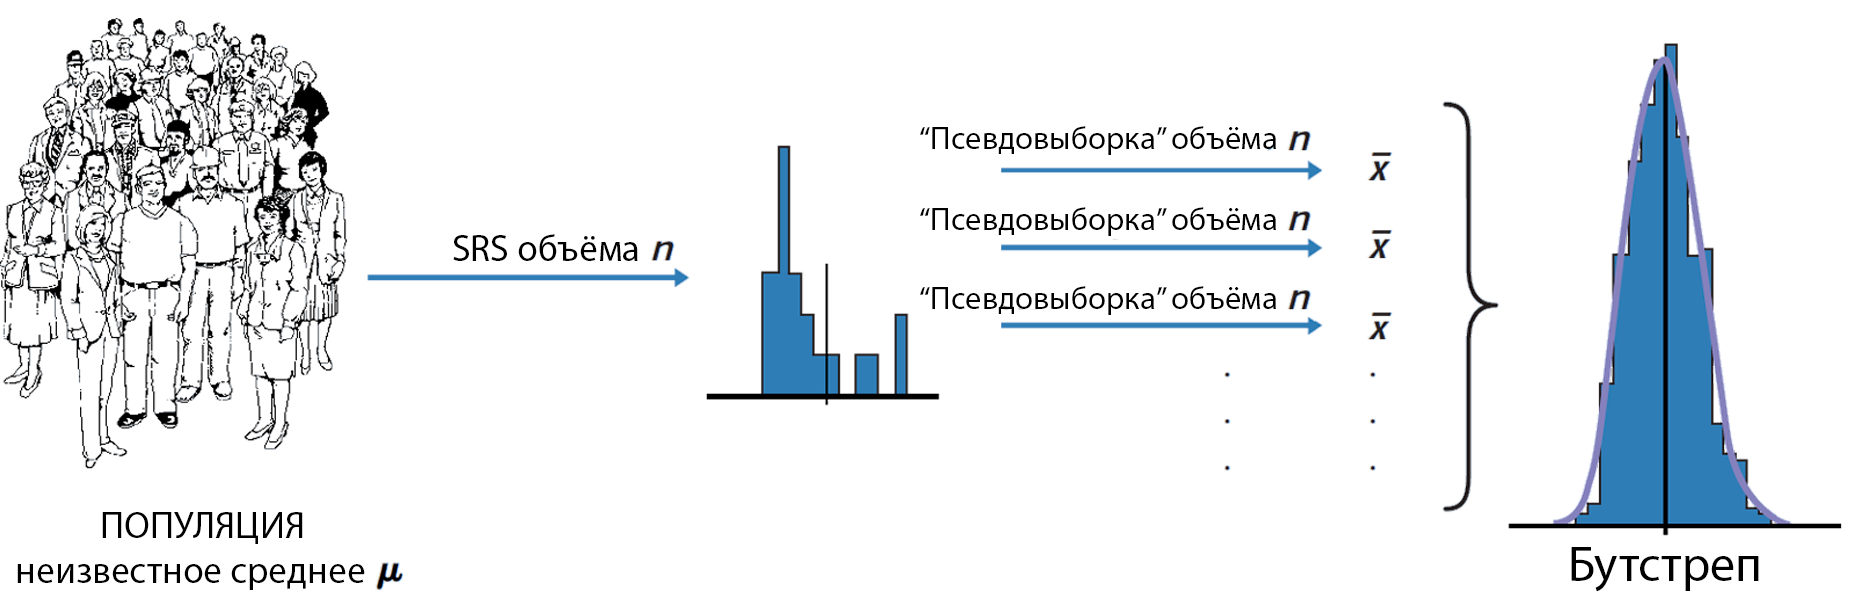
\includegraphics[width=1\textwidth]{boot3.png}
		\end{figure}
\end{frame}

\begin{frame}{Бутстреп}
%%%%%%%%%%%%%%%%%%%%%%%%%%%%%%%%%%%%%%%%%%%%%%%%%%%%%%%%%%%%%%%%%%%%%%%
% Почему это вообще работает? Давайте вспомним наш гипотетический наивный метод оценки распределения статистики. Когда мы извлекаем новые выборки из генеральной совокупности, мы сэмплируем из функции распределения нашей случайной величины. Когда доступа к генеральной совокупности нет, а есть только выборка объёма n, лучшая наша оценка F(x) - эмпирическая функция распределения. Если мы будем сэмплировать из неё, мы получим ровно те самые псевдовыборки с возвращениями из исходной выборки.
%%%%%%%%%%%%%%%%%%%%%%%%%%%%%%%%%%%%%%%%%%%%%%%%%%%%%%%%%%%%%%%%%%%%%%%
	Извлечение выборок из генеральной совокупности~--- сэмплирование из~неизвестного распределения $F_X\left(x\right).$

	Лучшая оценка $F_X\left(x\right),$ которая у~нас есть~--- $F_{X^n}\left(x\right)$:
	\begin{center}
		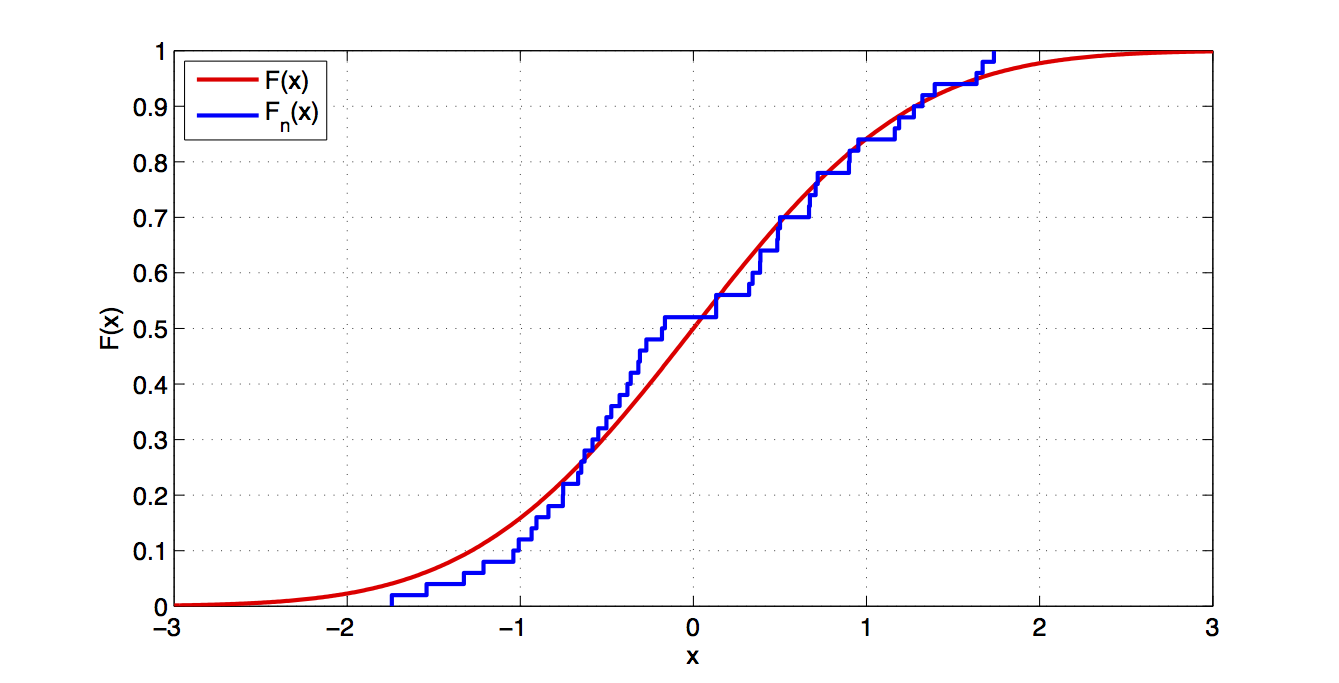
\includegraphics[width=0.8\textwidth]{ecdf.png}
	\end{center}
	Сэмплировать из неё~--- это то же самое, что делать из $X^n$ выборки с~возвращением объёма $n$.
\end{frame}

\begin{frame}{Бутстреп-распределение}
%%%%%%%%%%%%%%%%%%%%%%%%%%%%%%%%%%%%%%%%%%%%%%%%%%%%%%%%%%%%%%%%%%%%%%%
% Имея бутстрем-оценку распределения статистики, можно построить доверительный интервал для значения параметра, который она оценивает. Есть несколько способов.
%%%%%%%%%%%%%%%%%%%%%%%%%%%%%%%%%%%%%%%%%%%%%%%%%%%%%%%%%%%%%%%%%%%%%%%
	$X^{1*}, \dots, X^{N*}$~--- бутстреп-псевдовыборки из $X^n$ объёма $n$,

	$\hat{\theta}_n^{1*}, \dots, \hat{\theta}_n^{N*}$~--- значения статистики на них,

	$F_{\hat{\theta}_n}^{boot}(x)$~--- бутстреп-распределение $\hat{\theta}_n$~--- эмпирическая функция распределения, построенная по значениям статистики на псевдовыборках.

	\bigskip

	\begin{figure}
		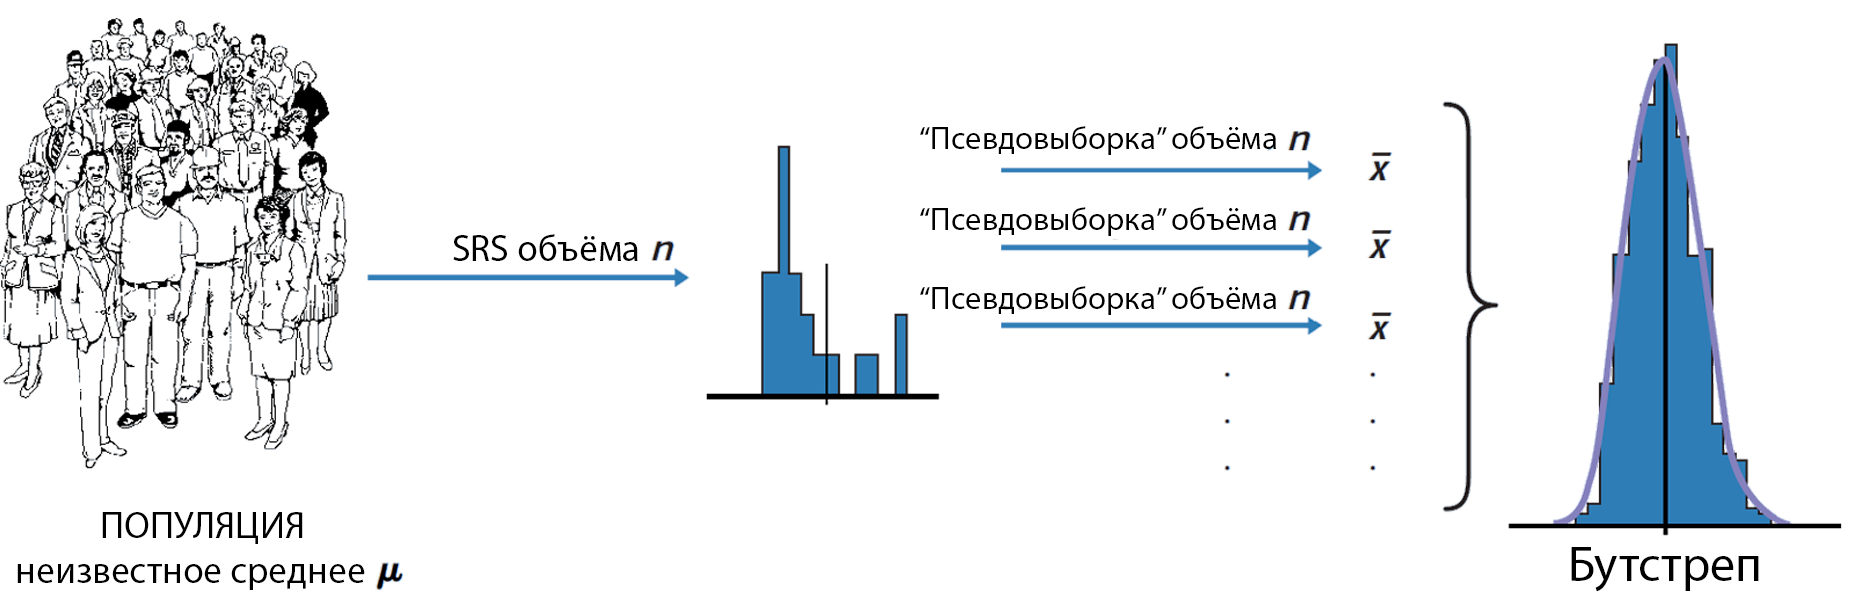
\includegraphics[width=0.95\textwidth]{boot3.png}
	\end{figure}

	\bigskip

	По $F_{\hat{\theta}_n}^{boot}(x)$ можно строить доверительные интервалы для $\theta$
\end{frame}

\begin{frame}{Доверительные интервалы}{Базовый бутстреп}
%%%%%%%%%%%%%%%%%%%%%%%%%%%%%%%%%%%%%%%%%%%%%%%%%%%%%%%%%%%%%%%%%%%%%%%
%Можно использовать всю информацию о распределении значений статистики на псевдовыборках: возьмём квантили нужного порядка от соответствующего бутстреп-распределения и получим искомый доверительный интервал. Так устроен базовый, или наивный бутстреп.

% Во-первых, псевдовыборки можно использовать только для оценки дисперсии распределения статистики, а потом строить доверительный интервал для параметра, прибавляя и вычитая из значения статистики на исходной выборке корень из этой бутстреп-дисперсии, умноженный на квантиль распределения Стьюдента. Это стьюдентизированный бутстреп.
%%%%%%%%%%%%%%%%%%%%%%%%%%%%%%%%%%%%%%%%%%%%%%%%%%%%%%%%%%%%%%%%%%%%%%%
Возьмём выборочные квантили бутстреп-распределения:
			$$\prob\left(\left(F_{\hat{\theta}_n}^{boot}\right)^{-1}\left(\frac{\alpha}{2}\right) \leq \theta \leq \left(F_{\hat{\theta}_n}^{boot}\right)^{-1}\left(1-\frac{\alpha}{2}\right) \right)\approx 1-\alpha.$$
			Это базовый бутстреп.
\end{frame}
\begin{frame}{Доверительные интервалы}{Cтьюдентизированный бутстреп}

Посчитаем $S_n^{boot}$~--- выборочное стандартное отклонение $\hat{\theta}_n$ на псевдовыборках;
			$$\prob \left(\hat{\theta}_n - t_{n-1, 1-\frac{\alpha}{2}} S_n^{boot}  \leq \theta \leq \hat{\theta}_n + t_{n-1, 1-\frac{\alpha}{2}} S_n^{boot}\right)\approx 1-\alpha.$$
			Это стьюдентизированный бутстреп.
\end{frame}
\begin{frame}{Доверительные интервалы}{bias-corrected accelerated bootstrap (BCa)}

    %%%%%%%%%%%%%%%%%%%%%%%%%%%%%%%%%%%%%%%%%%%%%%%%%%%%%%%%%%%%%%%%%%%%%%%
    % Если внести в процедуру наивного бутстрепа некоторые изменения, можно получить несмещённый ускоренный бутстреп, который всегда будет давать более точные доверительные интервалы (почему - можете прочитать в учебнике Эфрона и Тибширани). Функции, которые строят бутстреп-доверительные интервалы, как правило, делают это сразу всеми возможными способами; рекомундую всегда выбирать BCa - тот самый bias-corrected accelerated вариант.
    %%%%%%%%%%%%%%%%%%%%%%%%%%%%%%%%%%%%%%%%%%%%%%%%%%%%%%%%%%%%%%%%%%%%%%%
    Слегка изменим наивный бутстреп:
	$$
        \prob\left(\left(F_{\hat{\theta}_n}^{boot}\right)^{-1}\left(\alpha_1\right) \leq \theta \leq \left(F_{\hat{\theta}_n}^{boot}\right)^{-1}\left(\alpha_2\right) \right)\approx 1-\alpha,
    $$
    \vspace{-10pt}
    $$
        \alpha_1  = \Phi\left(\hat{z}_0 + \frac{\hat{z}_0 + z_{\frac{\alpha}{2}}}{1 - \hat{a} \left(\hat{z}_0 + z_{\frac{\alpha}{2}}\right)}\right),
        \qquad
        \alpha_2  = \Phi\left(\hat{z}_0 + \frac{\hat{z}_0 + z_{1-\frac{\alpha}{2}}}{1 - \hat{a} \left(\hat{z}_0 + z_{1-\frac{\alpha}{2}} \right)} \right),
    $$
    $$
        \hat{a} =
        \frac{\sum_{i=1}^n (\hat{\theta}_{(\cdot)} - \hat{\theta}_{(i)})^3}%
        {6\left(\sum_{i=1}^n (\hat{\theta}_{(\cdot)} - \hat{\theta}_{(i)})^2\right)^{3/2}},
        \qquad
        \hat\theta_{(\cdot)} = \frac{1}{n}\sum_{i=1}^n \hat\theta_{(i)}
    $$
    $$
        \hat{z}_0 = \Phi^{-1} \left(\frac1{N} \sum_{i=1}^N \left[ \hat{\theta}_n^{i*} < \hat{\theta}_n\right]\right),
	$$
%			\hat{a}   & \text{ не поместится на этом слайде}.\\
			Это несмещённый ускоренный бутстреп.
\end{frame}

\begin{frame}{Свойства бутстрепа}
%%%%%%%%%%%%%%%%%%%%%%%%%%%%%%%%%%%%%%%%%%%%%%%%%%%%%%%%%%%%%%%%%%%%%%%
% Бутсреп - крайне мощное средство оценки распределений практически каких угодно статистик, в том числе самых диких, не подвластных параметрической статистике (например, количество мод у распределения). Единственное его существенное ограничение в том, что он плохо работает в ситуациях, когда значение статистики зависит от маленького количества элементов выборки. Например, бутстреп-интервал для медианы будет не очень хорош, потому что медиана определяется только 1-2 значениями выборки. Ещё нагляднее это видно для такой статистики, как, допустим, максимум: сколько бы вы не бутстрапировали исходную выборку, ни на одной псевдовыборке вы не сможете получить значение статистики больше, чем исходное, да и вообще разных значений статистики на псевдовыборках, скорее всего будет не так много. Таким бутстрепом максимум исходной случайной величины хорошо не оценишь.
%%%%%%%%%%%%%%%%%%%%%%%%%%%%%%%%%%%%%%%%%%%%%%%%%%%%%%%%%%%%%%%%%%%%%%%
	\begin{itemize}
		\item асимптотическая состоятельность
		\item простота использования даже для самых сложных статистик
		\item плохо работает для статистик, значение которых зависит от~небольшого числа элементов выборки
	\end{itemize}
\end{frame}
\begin{frame}{Бутстреп в Python}{}
    {\centering \ttfamily \structure{scipy.stats.bootstrap()}\par}

    \bigskip
    Основные параметры:
    \begin{itemize}
        \item \texttt{data}~--- выборка
        \item \texttt{statistic}~--- функция, вычисляющая оцениваемую статистику.
        \item \texttt{n\_resamples}~--- число выборок
        \item \texttt{method}: \texttt{'percentile'}, \texttt{'basic'} или, \texttt{'bca'}~--- метод реализации бутстреп.
    \end{itemize}
\end{frame}

\begin{frame}[allowframebreaks]{Литература}
        Справочники по статистике:
        \begin{itemize}
            \item Кобзарь А.И. \textit{Прикладная математическая статистика}, 2006.
            \item Kanji G.K. \textit{100 statistical tests}, 2006.
        \end{itemize}

        Вводные учебники по статистике:
        \begin{itemize}
            \item Good P.I., Hardin J.W. \textit{Common Errors in Statistics (and How to Avoid Them)}, 2003.
            \item Reinhart A. \textit{Statistics Done Wrong. The woefully complete guide}, \small{\url{http://www.statisticsdonewrong.com/}\par}
        \end{itemize}
        Бутстреп:
        \begin{itemize}
            \item Hesterberg T., Monaghan S., Moore D.S., Clipson A., Epstein R. \textit{Bootstrap methods and permutation tests}. In Introduction to the Practice of Statistics, 2005. \small{\url{http://statweb.stanford.edu/~tibs/stat315a/Supplements/bootstrap.pdf}\par}
            \item Efron B., Tibshirani R. \textit{An Introduction to the Bootstrap}, 1993.
            \small{\url{https://vk.com/doc168073_278498071?hash=D2ZRo8Z3eoYf8uKtzutRj2lTMjN21W4ABiIvlZ41mTc&dl=rrTIbZplsbXxHonDZeWbAvTkH7lL4nZOZmIszqwBi8T&api=1&no_preview=1}\par}
        \end{itemize}

%        \bigskip
%
%        Проверка гипотез:
%        \begin{itemize}
%            \item Good P.I., Hardin J.W. \textit{Common Errors in Statistics (and How to Avoid Them)}, 2003, глава 2.
%        \end{itemize}

        \framebreak
        Разное:
        \begin{itemize}
            \item Begg I.M., Anas A., Farinacci S. (1992). \textit{Dissociation of processes in belief: Source recollection, statement familiarity, and the illusion of truth}. Journal of Experimental Psychology: General, 121(4), 446–458.

            \item Ellis P.D. \textit{The Essential Guide to Effect Sizes: Statistical Power, Meta-Analysis, and the Interpretation of Research Results}, 2010.

            \item Хафф Д. \textit{Как лгать при помощи статистики,} 2015 \small{\url{https://books.yandex.ru/books/FhAUBcm9}\par}


            \item Kirk R.E. (1996). \textit{Practical Significance: A Concept Whose Time Has Come}. Educational and Psychological Measurement, 56(5), 746–759.

            \item Marriott, F. H. C. \textit{The Interpretation of Multiple Observations}, 1974.
    \end{itemize}
\end{frame}
\end{document}














\begin{frame}
    Если не хватило...
\end{frame}
\section{Проверка гипотез}
\begin{frame}
\centering
\textbf{Проверка гипотез}

\includegraphics[width=0.8\textwidth]{vs.png}
\begin{multicols}{2}
    \centering
    \structure{Нулевая гипотеза $H_0$}

    \columnbreak

    \alert{Конкурирующая гипотеза $H_1$}
\end{multicols}
\begin{block}{}
    Нулевая гипотеза считается верной, пока не будет доказано обратное сверх необходимых сомнений.
\end{block}
\end{frame}
\subsection{Теория}
\begin{frame}{Проверка гипотез}
%%%%%%%%%%%%%%%%%%%%%%%%%%%%%%%%%%%%%%%%%%%%%%%%%%%%%%%%%%%%%%%%%%%%%%%
% Проверка гипотез - основной инструмент этого курса, если в итоге вы в нём не разберётесь, считайте, что зря потратили время. Имеется выборка из случайной величины X, которая имеет неизвестное распределение P. Кроме того, выдвинута нулевая гипотеза об этом распределении (например, ”P принадлежит некоторому семейству распределений ?”) и альтернативная гипотеза (например, общая альтернатива ”P не принадлежит ?”). Требуется проверить, глядя на выборку, какая из двух гипотез, нулевая или альтернативная, более вероятна. Для этого используется некоторая статистика T , которая обладает очень важным свойством: если нулевая гипотеза справедлива, то точно известно, какое у статистики распределение, а если справедлива альтернатива, то распределение статистики — какое-то другое. Распределение F (x) называется нулевым распределением статистики, а пара, состоящая из статистики и нулевого распределения, образует статистический критерий для проверки нулевой гипотезы против альтернативы. Мы получаем данные, то есть, реализацию выборки, считаем на них значение статистики и по нему вычисляем так называемый достигаемый уровень значимости, или p-value, представляющий собой вероятность получить такое или ещё более экстремальное значение статистики при справедливости нулевой гипотезы. "Экстремальность" определяется относительно альтернативной гипотезы: допустим, если при альтернативе более вероятными являются большие значения статистики, то именно их мы и будем считать экстремальными. Затем p-value сравнивают с порогом ?, который называется уровнем значимости. Чаще всего ? = 0.05. Если p ? ?, то нулевая гипотеза отвергается в пользу альтернативы. Если p > ?, то нулевая гипотеза не отвергается.
%%%%%%%%%%%%%%%%%%%%%%%%%%%%%%%%%%%%%%%%%%%%%%%%%%%%%%%%%%%%%%%%%%%%%%%
	\only<1>{
		\begin{center}
			\vspace{-10pt}
			\begin{tabular}{rl}
				выборка:                        & $X^n=\left(X_1,\ldots,X_n\right), \; X \sim \prob \in \Omega$         \\
				нулевая гипотеза:               & $H_0\colon \prob\in\omega, \;\; \omega\in\Omega$ \\
				альтернатива:                   & $H_1\colon \prob\notin\omega$ \\
				статистика:                     & $T\left(X^n\right), \;\; T\left(X^n\right)\sim F\left(x\right) \;\text{при}\; \prob\in\omega$ \\
				& \;\;\;\;\;\;\;\;\;\;\;\;\;\; $T\left(X^n\right)\not\sim F\left(x\right) \;\text{при}\; \prob\notin\omega$ \\
				\multicolumn{2}{c}{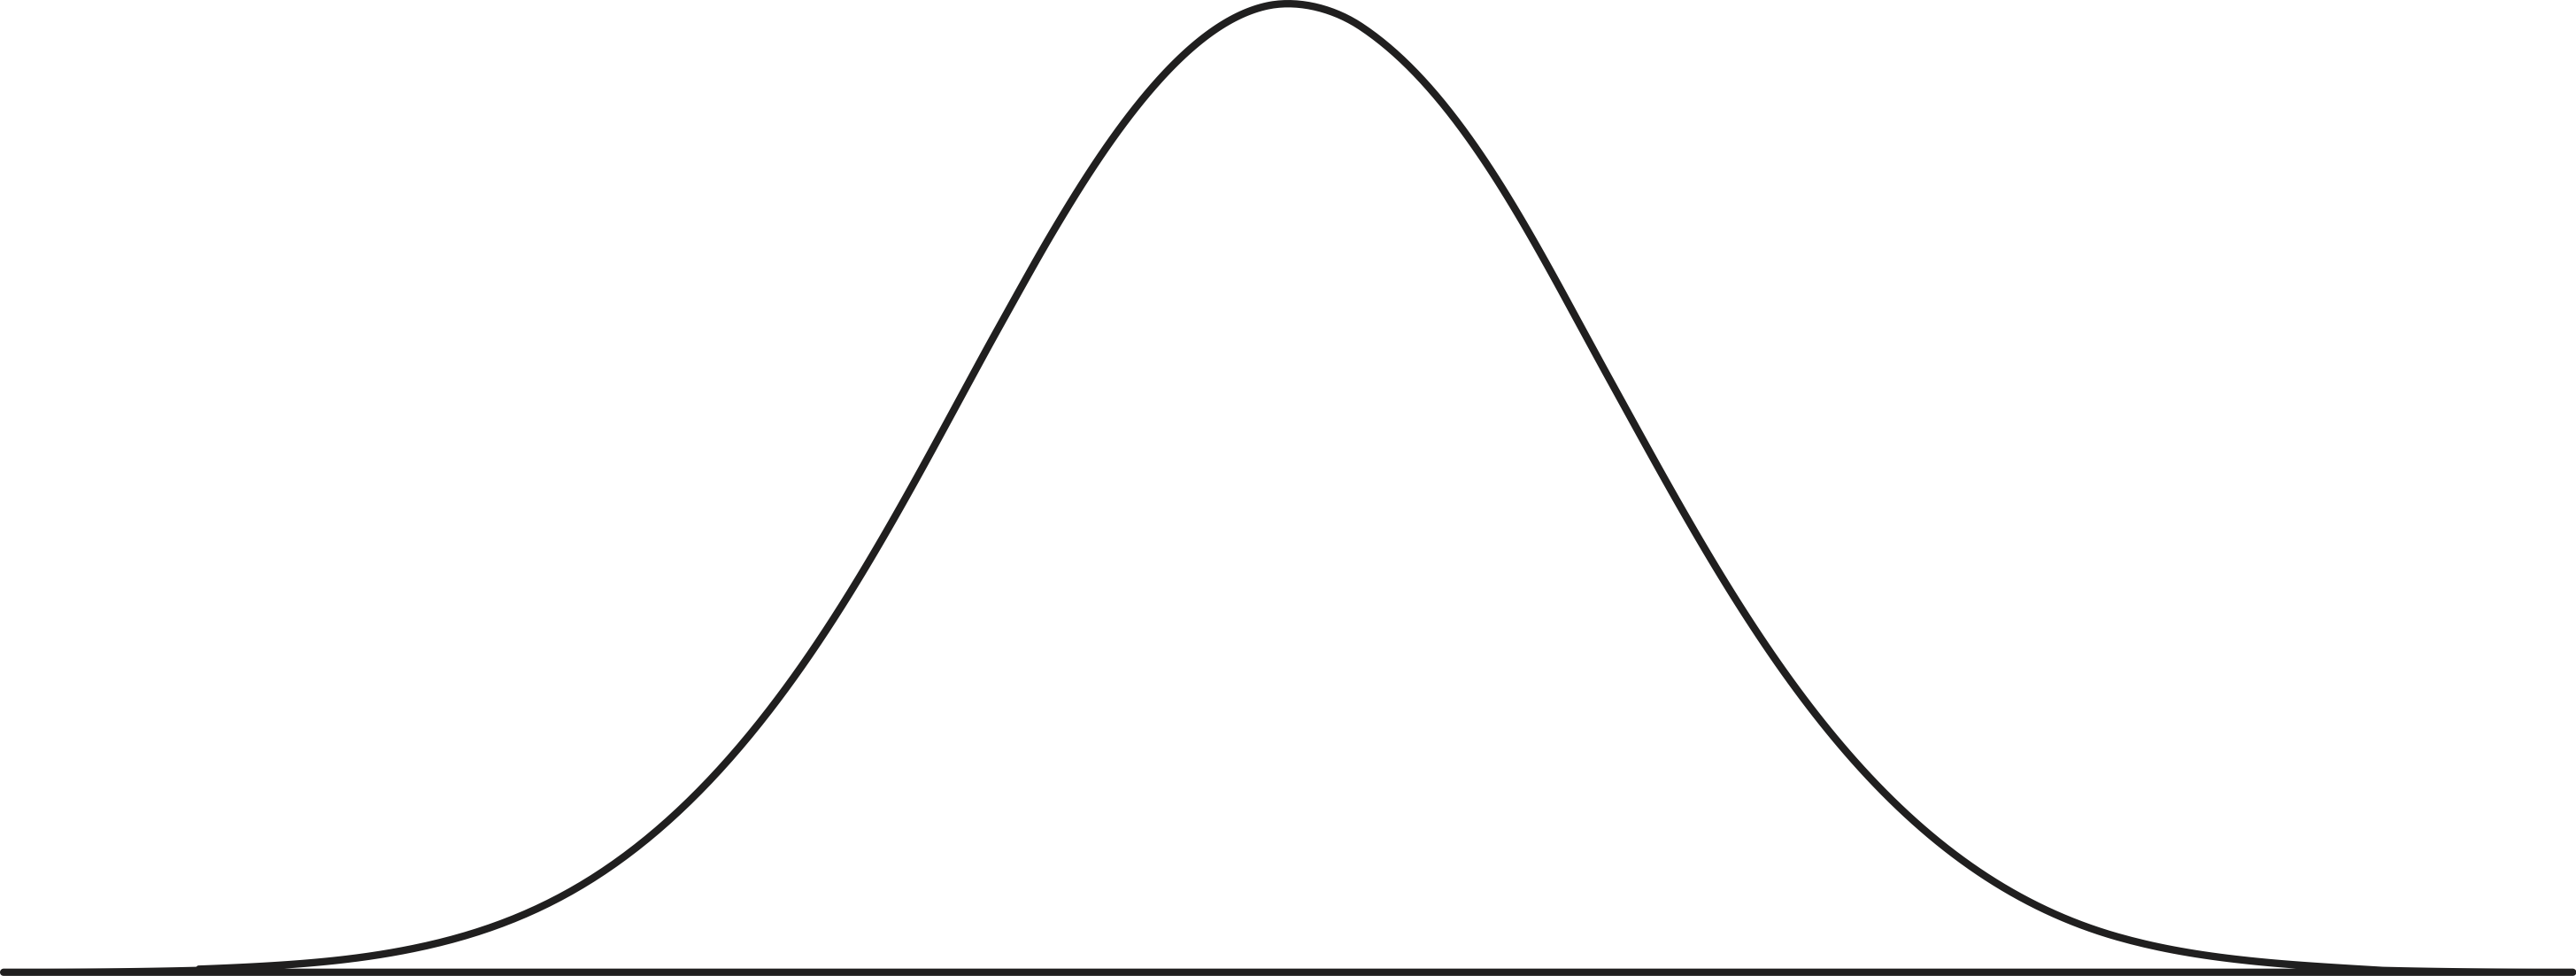
\includegraphics[width=0.3\textwidth]{stats1.png}} \\
				реализация выборки:             & $x^n=\left(x_1,\ldots,x_n\right)$ \\
				реализация статистики:          & $t = T \left(x^n\right)$ \\
				достигаемый уровень значимости: & $p\left(x^n\right)$~--- вероятность при $H_0$ получить \\
				& $T \left(X^n\right)=t$ или ещё более экстремальное\\
				\multicolumn{2}{c}{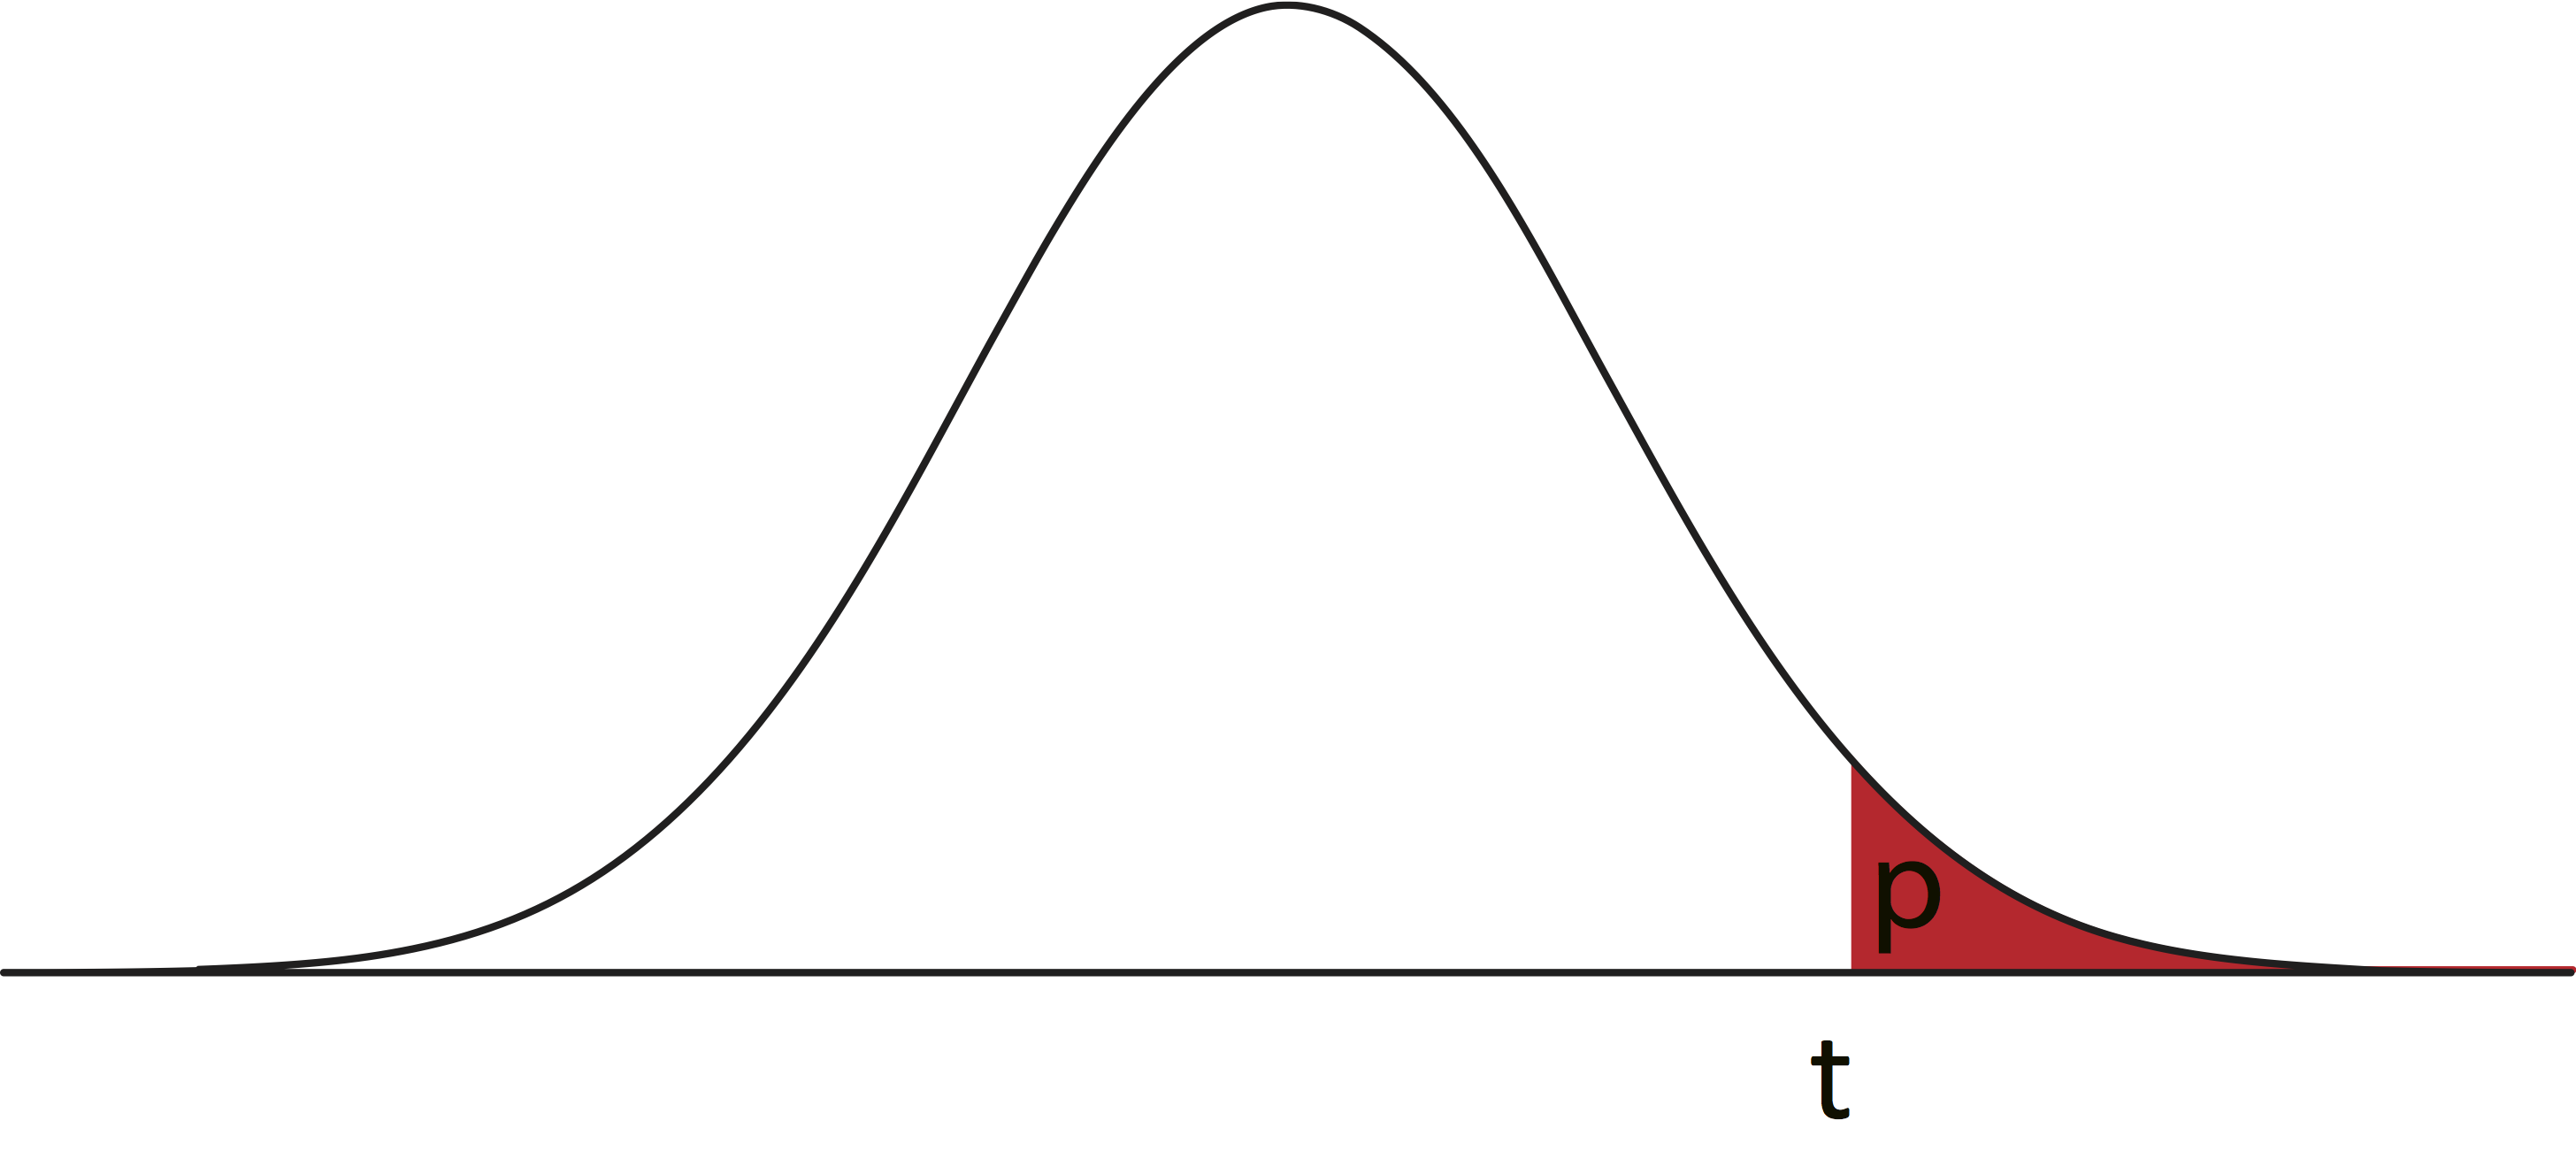
\includegraphics[width=0.3\textwidth]{stats2.png}} \\
				\multicolumn{2}{c}{ $p\left(x^n\right) = \prob\left(T\geq t\left|H_0\right.\right)$ } \\
				\multicolumn{2}{c}{Гипотеза отвергается при $p\left(x^n\right)\leq\alpha,\;\;\alpha$~--- уровень значимости} \\
			\end{tabular}
		\end{center}
	}
	\only<2>{
		\vspace{-3pt}
		\begin{center}
			\includegraphics[height=0.8\textheight]{rememberkids.png}
		\end{center}
	}
\end{frame}

\begin{frame}{Достигаемый уровень значимости}
%%%%%%%%%%%%%%%%%%%%%%%%%%%%%%%%%%%%%%%%%%%%%%%%%%%%%%%%%%%%%%%%%%%%%%%
% Достигаемый уровень значимости - достаточно сложная концепция. Например, авторы блога fivethirtyeight на конференции по мета-анализу провели опрос участников, спрашивая их, что такое достигаемый уровень значимости, и получили набор ответов от неправильных до "я не помню, нужно спросить моего аспиранта". И это исследователи - люди, которые часто сталкиваются со статистикой!
% Проблема определения p-value в том, что оно длинное, но из него ничего нельзя выбросить так, чтобы оно не стало неправильным. Например, часто хочется думать, что p-value — это просто вероятность справедливости нулевой гипотезы, но это не так! Это хорошо понятно на следующем примере. В 2010 году осьминог Поль угадывал результаты матчей чемпионата мира по футболу с участием сборной Германии, выбирая из двух кормушек ту, на которой был изображён флаг страны-победителя. Из 13 матчей, в которых он пробовал свои силы, результаты 11 ему удалось угадать. Используя эти данные как выборку, можно проверить нулевую гипотезу о том, что он выбирал кормушку наугад против альтернативы о том, у осьминога есть сверхспособности к предсказанию результатов матчей. Критерий, которым проверяется эта нулевая гипотеза, будет разобран позже. Но если его применить, получится достигаемый уровень значимости p = 0.0112. Это значение — не вероятность, что осьминог выбирает кормушку наугад. Вероятность того, что осьминог выбирает кормушку наугад, равна единице! p = 0.0112 — это именно вероятность получить такие или ещё более экстремальные данные при условии справедливости нулевой гипотезы. Эта вероятность достаточно мала, но редкие события тоже происходят. И, как правило, именно о них пишут в газетах.
%%%%%%%%%%%%%%%%%%%%%%%%%%%%%%%%%%%%%%%%%%%%%%%%%%%%%%%%%%%%%%%%%%%%%%%
$$p = \prob\left(T\geq t\left|H_0\right.\right) \neq \prob \left(H_0\right)$$

\textbf{Пример:} утверждается, что осьминог предсказывает результаты матчей с~участием сборной Германии на чемпионате мира по футболу 2010 года, выбирая кормушку с флагом страны-победителя.
По результатам $13$~испытаний ему удаётся верно угадать результаты $11$~матчей.  Применяя подходящий статистический критерий, мы получаем $p\approx 0.0112.$

\begin{center}
	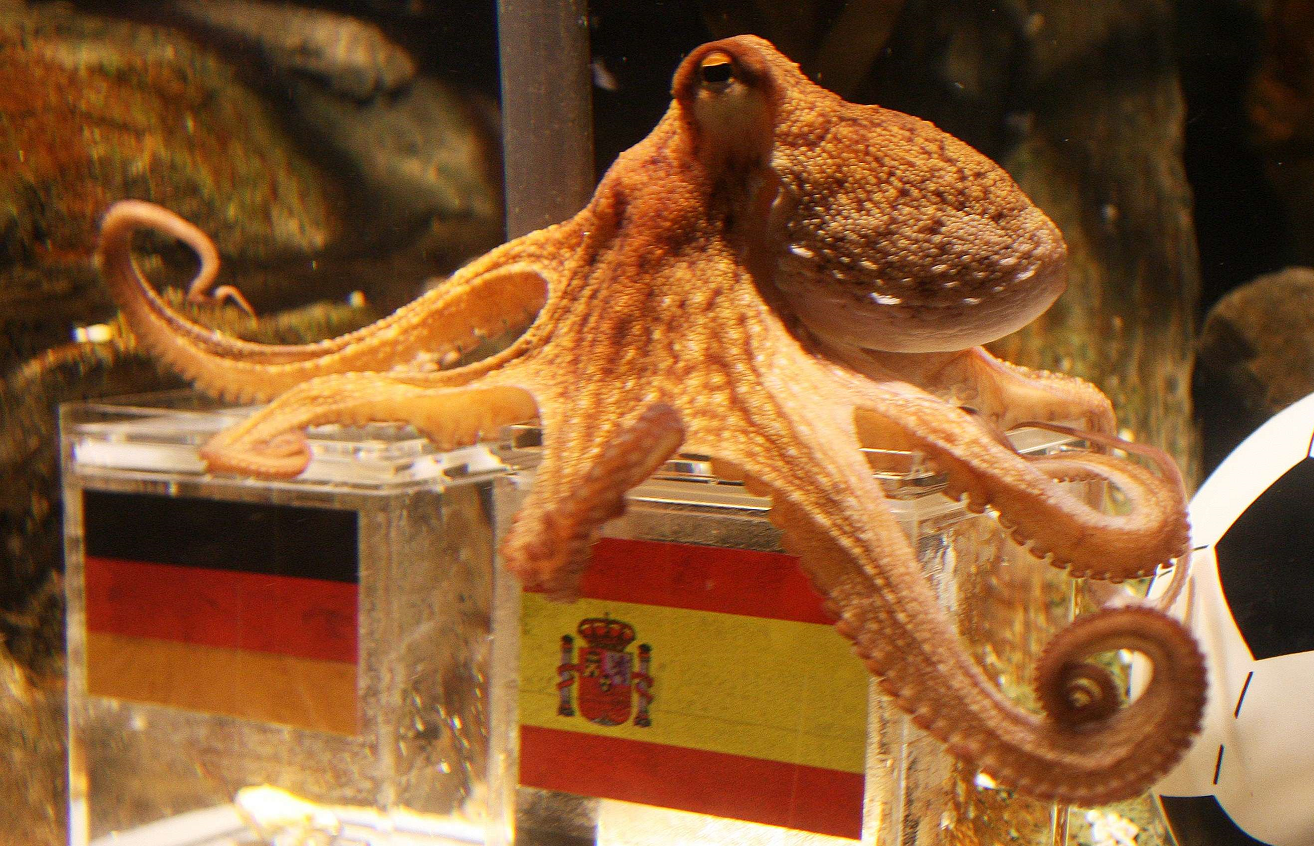
\includegraphics[height=0.35\textheight]{pauloctopus.png}
\end{center}

$0.0112$~--- не вероятность того, что осьминог выбирает кормушку
наугад! Эта вероятность равна единице.
\end{frame}

\begin{frame}{Ошибки I и II рода}
	\only<1>{
%%%%%%%%%%%%%%%%%%%%%%%%%%%%%%%%%%%%%%%%%%%%%%%%%%%%%%%%%%%%%%%%%%%%%%%
% Существенная особенность механизма проверки гипотез — его несимметричность относительно пары нулевая гипотеза – альтернатива. Эта особенность тесно связана с понятиями ошибок первого и второго рода.Нулевая гипотеза может быть либо верна, либо неверна. В результате проверки гипотезы ее? можно либо принять, либо отвергнуть.  На главной диагонали находятся верные решения: либо принимается верная нулевая гипотеза, либо отвергается неверная нулевая гипотеза. А вот на побочной диагонали располагаются ошибки. Совершить ошибку первого рода — значит отвергнуть верную нулевую гипотезу. Если же принимается неверная нулевая гипотеза, то это ошибка второго рода.
%%%%%%%%%%%%%%%%%%%%%%%%%%%%%%%%%%%%%%%%%%%%%%%%%%%%%%%%%%%%%%%%%%%%%%%

	\begin{center}
    \begin{tabular}{ |r | >{\centering}p{3.1cm} | >{\centering}p{3.1cm} | }
        \hline
        & $H_0$ верна         & $H_0$ неверна \tabularnewline \hline
        $H_0$ принимается & 
\includegraphics[height=3cm]{TP.png} & 
\includegraphics[height=3cm]{FN.png}\tabularnewline \hline
        $H_0$ отвергается & 
\includegraphics[height=3cm]{FP.png} Ошибка I рода (False positive) & 
\includegraphics[height=3cm]{TN.png}$H_0$ верно отвергнута\tabularnewline
        \hline
    \end{tabular}
    \end{center}
	}

	\only<2>{
%%%%%%%%%%%%%%%%%%%%%%%%%%%%%%%%%%%%%%%%%%%%%%%%%%%%%%%%%%%%%%%%%%%%%%%
% В механизме проверки гипотез ошибки первого и второго рода неравнозначны. Ошибка первого рода критичнее, вероятность отвержение нулевой гипотезы в случае, когда она верна, жестко ограничивается. Если нулевая гипотеза отвергается при значении уровня значимости p ? ?, то вероятность ошибки первого рода получается ограниченной сверху величиной ?. Таким образом, любой корректный, хорошо построенный критерий имеет вероятность ошибки первого рода не больше, чем уровень значимости. Что касается ошибки второго рода, то она минимизируется по остаточному принципу. Понятие ошибки второго рода связано с понятием мощности статистического критерия. Мощность — это вероятность отверг- нуть неверную нулевую гипотезу.  Чтобы найти идеальный критерий для проверки пары нулевая гипотеза – альтернатива, нужно среди всех корректных критериев выбрать критерий с максимальной мощностью.
%%%%%%%%%%%%%%%%%%%%%%%%%%%%%%%%%%%%%%%%%%%%%%%%%%%%%%%%%%%%%%%%%%%%%%%
		Задача проверки гипотез несимметрична относительно пары $\left(H_0,H_1\right)$: вероятность ошибки первого рода ограничивается сверху величиной $\alpha$, а второго рода~--- минимизируется путём выбора критерия.

		\bigskip

		\textbf{Корректный} критерий: $\prob\left(p\left(T\right)\leq\alpha\left|H_0\right.\right)\leq \alpha \forall \prob \in \Omega$.

		\textbf{Мощность}: $\pow = \prob\left(p\left(T\right)\leq\alpha\left|H_1\right.\right).$

		\textbf{Состоятельный} критерий: $\pow \rightarrow 1 $ для всех альтернатив $H_1$ при $n\rightarrow \infty$.

		$T_1$~--- \textbf{равномерно наиболее мощный} критерий, если $\forall T_2$
		\begin{align*}
		\prob\left(p\left(T_1\right)\leq \alpha\left|H_1\right.\right) & \geq \prob\left(p\left(T_2\right)\leq \alpha\left|H_1\right.\right) \;\; \forall H_1\neq H_0, \\
		\prob\left(p\left(T_1\right)\leq \alpha\left|H_0\right.\right) & = \prob\left(p\left(T_2\right)\leq \alpha\left|H_0\right.\right),
		\end{align*}
		причём хотя бы для одной $H_1$ неравенство строгое.
	}
\end{frame}
%
%\begin{frame}{Матрица ошибок}{}
%    \begin{tabular}{|>{\columncolor{blue}}l|m{35mm}|m{35mm}|}
%        \hline
%        \rowcolor{blue}& $\color{white} H_0$ \color{white}  верна & $\color{white} H_0$ \color{white} неверна\\
%        \hline
%        $\color{white} H_0$ \color{white} принята & Верное решение &  \cellcolor{red!30} Ошибка II рода \\
%        \hline
%        $\color{white} H_0$ \color{white} отвергнута & \cellcolor{red!30}  Ошибка I рода &  Верное решение\\
%        \hline
%    \end{tabular}
%
%    \vfill
%    \begin{itemize}
%        \item \alert{Ошибка первого рода}~--- отвержение верной гипотезы $H_0$.
%        \item \alert{Ошибка второго рода}~--- принятие ошибочной гипотезы $H_0$.
%    \end{itemize}
%
%    \vfill
%
%    % Какая из ошибок является более опасной, зависит от конкретной задачи.
%
%    \vfill
%    {\centering
%        \begin{tikzpicture}
%            \begin{axis}[
%                name=myaxis,
%                no markers, domain=-2:4, samples=500,
%                axis y line=none,
%                axis x line=center,
%                xlabel=$T$, %ylabel=$p$,
%                every axis y label/.style={at=(current axis.above origin),anchor=south},
%                every axis x label/.style={at=(current axis.right of origin),anchor=west},
%                height=5cm, width=11cm,
%                xmin=-2.1, xmax=4.1,
%                ymin=-0.1, ymax=0.5,
%                xtick=\empty, ytick=\empty,
%                enlargelimits=false, clip=false, axis on top,
%                grid = none
%                ]
%                \addplot [fill=cyan!20, draw=none, domain=1.4:3] {gauss(0,1)} \closedcycle;
%                \addplot [fill=red!20, draw=none, domain=0:1.4] {gauss(3,1)} \closedcycle;
%                \addplot [very thick,cyan!50!black] {gauss(0,1)};
%                \addplot [very thick,red!50!black] {gauss(3,1)};
%
%                \draw[thick,red!50, rounded corners = 4mm] (axis cs:4,-0.05) -| (axis cs:1.4,0);
%                \draw[thick,cyan!50, rounded corners = 4mm] (axis cs:-2,-0.05) -| (axis cs:1.4,0);
%
%                % \fill[cyan!20] (axis cs:1.4,-0.02) rectangle (axis cs:-2,0);
%
%                \node[coordinate,pin=135:{Ошибка II рода}]
%                at (axis cs:1.2,0.02) {};
%                \node[coordinate,pin=45:{Ошибка I рода}]
%                at (axis cs:1.6,0.04) {};
%                \draw[red] (axis cs:1.4,-0.04) node[below]{$T_\text{кр.}$} -- (axis cs:1.4,0.5);
%            \end{axis}
%        \end{tikzpicture}
%        \par}
%\end{frame}

\begin{frame}{Интерпретация результата}
%%%%%%%%%%%%%%%%%%%%%%%%%%%%%%%%%%%%%%%%%%%%%%%%%%%%%%%%%%%%%%%%%%%%%%%
% Неравнозначность нулевой и альтернативной гипотезы видна уже на уровне терминологии. Если достига- емый уровень значимости p <= alpha, то говорят, что нулевая гипотеза отвергается в пользу альтернативы. Если достигаемый уровень значимости p > alpha, то нулевая гипотеза не отвергается. Когда гипотеза не отвергается, это значит только то, что нет доказательств того что она неверна. Но отсутствие доказательств не является доказательством ее верности! Это можно лучше понять на примере судебного процесса. Основное положение — презумпции невинов- ности: подсудимый по умолчанию невиновен (это нулевая гипотеза), и, если доказательств обратному нет, нельзя утверждать, что он преступник, даже если он на самом деле совершил преступление.
%%%%%%%%%%%%%%%%%%%%%%%%%%%%%%%%%%%%%%%%%%%%%%%%%%%%%%%%%%%%%%%%%%%%%%%
    \begin{itemize}
	\item Если величина $p$ достаточно мала, то данные свидетельствуют против нулевой гипотезы в пользу альтернативы.

	\item Если величина $p$ недостаточно мала, то данные не свидетельствуют против нулевой гипотезы в пользу альтернативы.
    \end{itemize}
	\bigskip

	При помощи инструмента проверки гипотез нельзя доказать справедливость нулевой гипотезы!

	Absence of evidence $\nRightarrow$ evidence of absence.
\end{frame}

\begin{frame}{Статистическая и практическая значимость}
	\only<1>{
%%%%%%%%%%%%%%%%%%%%%%%%%%%%%%%%%%%%%%%%%%%%%%%%%%%%%%%%%%%%%%%%%%%%%%%
% На самом деле эксперименты проводятся не для того, чтобы получить значение p-value. Как правило, исследователя интересует размер эффекта, то есть степень отклонения данных от нулевой гипотезы. Например, если эксперимент связан с проверкой способностей предсказателя будущего, то размер эффекта — это вероятность верного предсказания. Если проверяется эффективность лекарства, то размер эффекта — это вероятность выздоровления пациента, который это лекарство принимает, за вычетом эффекта плацебо. При запуске программы лояльности для пользователей интернет-магазина размер эффекта — это последующее увеличение среднего чека.
% Размер эффекта — это величина, определенная на генеральной совокупности. Но, как правило, у исследователя есть только небольшая выборка из нее, а оценка размера эффекта по выборке — это случайная величина. Маленький достигаемый уровень значимости является показателем того, что такую оценку размера эффекта, какая получена по выборке, с маленькой вероятностью можно было получить случайно. Достигаемый уровень значимости зависит не только от размера эффекта, но и от объема выборки, по которой оценивается эффект. Если выборка небольшая, скорее всего, нулевая гипотеза на ней не отвергается (если только она не слишком дикая). Однако с ростом объема выборки начинают проявляться все более тонкие отклонения данных от нулевой гипотезы. Велика вероятность, что на достаточно большой выборке значительная часть разумных нулевых гипотез будет отвергнута. Именно поэтому, даже если нулевая гипотеза отвергнута, это еще не значит, что полученный эффект имеет какую-то практическую значимость, её нужно оценивать отдельно.
%%%%%%%%%%%%%%%%%%%%%%%%%%%%%%%%%%%%%%%%%%%%%%%%%%%%%%%%%%%%%%%%%%%%%%%
		Вероятность отвергнуть нулевую гипотезу зависит не только от того, насколько она отличается от истины, но и от размера выборки.

		По мере увеличения $n$ нулевая гипотеза может сначала приниматься, но потом выявятся более тонкие несоответствия выборки гипотезе $H_0$, и она будет отвергнута.

		\bigskip

		При любой проверке гипотез нужно оценивать \textbf{размер эффекта}~--- степень отличия нулевой гипотезы отличается от истины, и оценивать его практическую значимость.
	}

	\only<2>{
%%%%%%%%%%%%%%%%%%%%%%%%%%%%%%%%%%%%%%%%%%%%%%%%%%%%%%%%%%%%%%%%%%%%%%%
% Первый пример связан с большим исследованием, в рамках которого на протяжении трех лет у большой выборки женщин измеряли вес, а также оценивали, насколько активно они занимаются спортом. По итогам исследования выяснилось, что женщины, которые в течение этого времени упражнялись не меньше часа в день, набрали значительно меньше веса, чем женщины, которые упражнялись менее 20 минут в день. Статистическая значимость этого результата достаточно высока: p < 0.001. Проблема в размере эффекта: разница в набранном весе между двумя исследуемыми группами женщин составила всего 150 граммов. 150 граммов за 3 года — это не очень много. Крайне сомнительно, что этот эффект имеет какую-то практическую значимость.
%Еще один пример связан с клиническими испытаниями гормонального препарата «Премарин», который облегчает симптомы менопаузы. В 2002 году эти испытания были прерваны досрочно, поскольку было обна- ружено, что прием препарата ведет к значимому увеличению риска развития рака груди (на 0.08%), инсульта (на 0.08%) и инфаркта (на 0.07%). Этот эффект статистически значим; при этом на первый взгляд кажется, что размеры эффектов ничтожны. Например, если кому-то сказать, что его любимые конфеты повышают риск возникновения инфаркта на 0.07%, вряд ли это заставит человека отказаться от этих конфет. Тем не менее, если пересчитать размеры эффектов на всю популяцию людей, которым этот препарат может быть по- тенциально приписан, результатом будут тысячи дополнительных смертей. Разработчики препарата не могут взять на себя эту ответственность, поэтому такой препарат немедленно запрещают и снимают с рынка.
% Этот пример показывает, что практическую значимость результата нельзя определить на глаз. В идеале она должна определяться человеком, который поставил задачу и понимает предметную область.
% Еще один пример — это испытание лекарства, которое замедляет ослабление интеллекта у людей, страдающих болезнью Альцгеймера. В этом исследовании очень сложно измерить размер эффекта. В течение эксперимента одна часть испытуемых должна принимать лекарство, а другая — плацебо. Только по прошествии нескольких лет можно будет сравнить эти две группы. Поэтому такое исследование длится долгое время и дорого стоит. Если при испытании оказывается, что разница между снижением IQ в контрольной группе, где люди принимали плацебо, и тестовой группе, где люди принимали препарат, составляет 13 пунктов, это различие очень большое, и на практике этот эффект крайне значим. При этом может оказаться, что статистическая значимость не была достигнута, то есть p > alpha, и формально нулевую гипотезу об отсутствии эффекта лекарства нельзя отвергнуть. Если предмет исследования очень важен, то, оказавшись в подобной ситуации, возможно, стоит продолжать исследования: набрать еще выборку, уменьшить дисперсию оценки размера эффекта и убедиться в том, что важное открытие не упущено.
%%%%%%%%%%%%%%%%%%%%%%%%%%%%%%%%%%%%%%%%%%%%%%%%%%%%%%%%%%%%%%%%%%%%%%%
		\begin{itemize}
			\item (Lee et al, 2010): за три года женщины, упражнявшиеся не меньше часа в день, набрали значимо меньше веса, чем женщины, упражнявшиеся меньше 20~минут в день ($p<0.001$).
			Разница в~набранном весе составила 150~г.
			Практическая значимость такого эффекта сомнительна. Подробности: \url{http://youtu.be/oqDZO-mfN4Q}.
			\item (Ellis, 2010, гл.~2): в 2002 году клинические испытания гормонального препарата Премарин, облегчающего симптомы менопаузы, были досрочно прерваны.
			Было обнаружено, что его приём ведёт к~значимому увеличению риска развития рака груди на~0.08\%, риска инсульта на~0.08\% и~инфаркта на~0.07\%.
			Формально эффект крайне мал, но с~учётом численности населения он превращается в тысячи дополнительных смертей.
			\item (Kirk, 1996): если при испытании гипотетического лекарства, позволяющего замедлить прогресс ослабления интеллекта больных Альцгеймером, оказывается, что разница в IQ контрольной и тестовой групп составляет 13~пунктов, возможно, изучение лекарства стоит продолжить, даже если эта разница статистически незначима.
		\end{itemize}
	}
\end{frame}

\begin{frame}{Другие особенности}
%%%%%%%%%%%%%%%%%%%%%%%%%%%%%%%%%%%%%%%%%%%%%%%%%%%%%%%%%%%%%%%%%%%%%%%
%
%%%%%%%%%%%%%%%%%%%%%%%%%%%%%%%%%%%%%%%%%%%%%%%%%%%%%%%%%%%%%%%%%%%%%%%
	\begin{itemize}
		\item Выбранная статистика может отражать не всю информацию, содержащуюся в выборке. Пример:
		$$H_0\colon X\sim N\left(\mu, \sigma^2\right), \;\; H_1\colon H_0 \text{ неверна;}$$
		$$T\left(X^n\right)=g_1.$$
		Все симметричные распределения будут признаны нормальными!
		\item Гипотезы вида $H_0\colon \theta=\theta_0$ можно проверять при помощи доверительных интервалов для $\theta$:
		\begin{itemize}
			\item если $\theta_0$ не попадает в $100\left(1-\alpha\right)$\% доверительный интервал для $\theta$, то $H_0$ отвергается на уровне значимости $\alpha$;
			\item p-value~--- максимальное $\alpha$, при котором $\theta_0$ попадает в~соответствующий доверительный интервал.
		\end{itemize}
	\end{itemize}
\end{frame}

\subsection{Пример}
\begin{frame}{Shaken, not stirred}
%%%%%%%%%%%%%%%%%%%%%%%%%%%%%%%%%%%%%%%%%%%%%%%%%%%%%%%%%%%%%%%%%%%%%%%
%
%%%%%%%%%%%%%%%%%%%%%%%%%%%%%%%%%%%%%%%%%%%%%%%%%%%%%%%%%%%%%%%%%%%%%%%
	Джеймс Бонд говорит, что предпочитает мартини взболтанным, но не смешанным. Проведём слепой тест: $n$ раз предложим ему пару напитков и~выясним, какой из двух он предпочитает.

	\bigskip

	Выборка: бинарный вектор длины $n$, $1$~--- Джеймс Бонд предпочёт взболтанный, $0$~--- смешанный.

	\bigskip

	Нулевая гипотеза: Джеймс Бонд не различает два вида мартини, т.\,е., выбирает наугад.

	\bigskip

	Статистика $T$~--- число единиц в выборке.
\end{frame}

\begin{frame}{Нулевое распределение}
%%%%%%%%%%%%%%%%%%%%%%%%%%%%%%%%%%%%%%%%%%%%%%%%%%%%%%%%%%%%%%%%%%%%%%%
%
%%%%%%%%%%%%%%%%%%%%%%%%%%%%%%%%%%%%%%%%%%%%%%%%%%%%%%%%%%%%%%%%%%%%%%%
	Если нулевая гипотеза справедлива и Джеймс Бонд не различает два вида мартини, то равновероятны все выборки длины $n$ из нулей и единиц.

	\bigskip

	Пусть $n=16$, тогда существует $2^{16} = 65536$ равновероятных варианта. Статистика $T$ принимает значения от $0$ до $16$:

	\begin{center}
		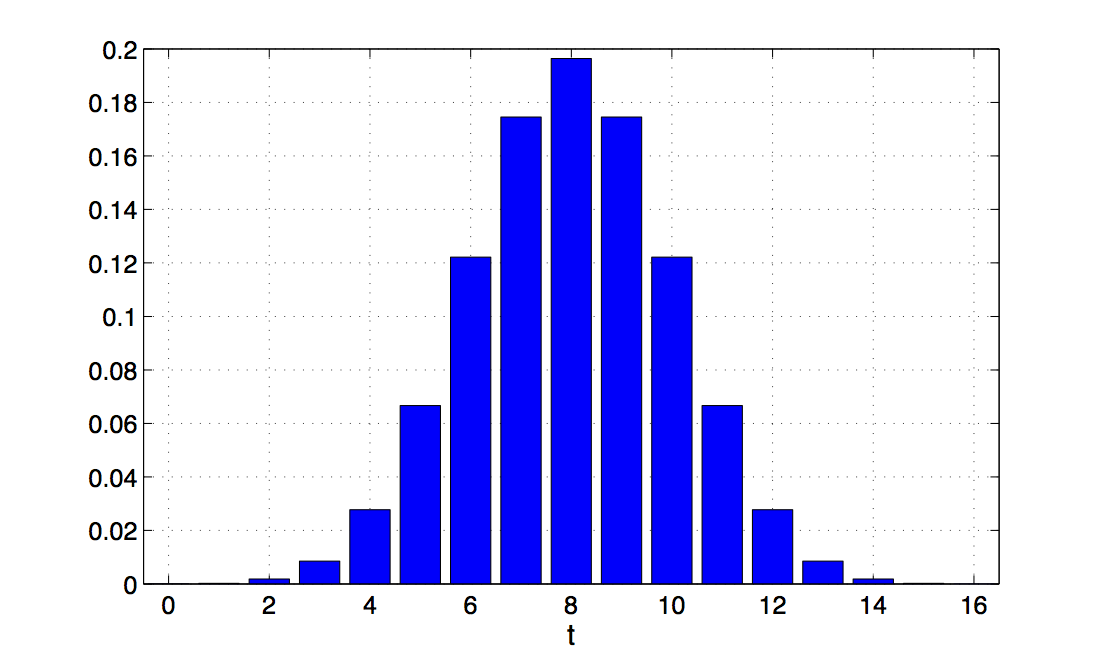
\includegraphics[height=0.6\textheight]{bond1.png}
	\end{center}

\end{frame}

\begin{frame}{Односторонняя альтернатива}
%%%%%%%%%%%%%%%%%%%%%%%%%%%%%%%%%%%%%%%%%%%%%%%%%%%%%%%%%%%%%%%%%%%%%%%
% достигаемый уровень значимости здесь - это суммарная высота всех красных столбиков
%%%%%%%%%%%%%%%%%%%%%%%%%%%%%%%%%%%%%%%%%%%%%%%%%%%%%%%%%%%%%%%%%%%%%%%
	$H_1\colon$ Джеймс Бонд предпочитает взболтанный мартини.

	При справедливости такой альтернативы более вероятны большие значения $T$ (т.е., большие $T$ свидетельствуют против $H_0$ в пользу $H_1$).

	Вероятность того, что Джеймс Бонд предпочтёт взболтанный мартини в $12$ или более случаях из $16$ при справедливости $H_0$, равна $\frac{2517}{65536}\approx 0.0384$.
	\begin{center}
		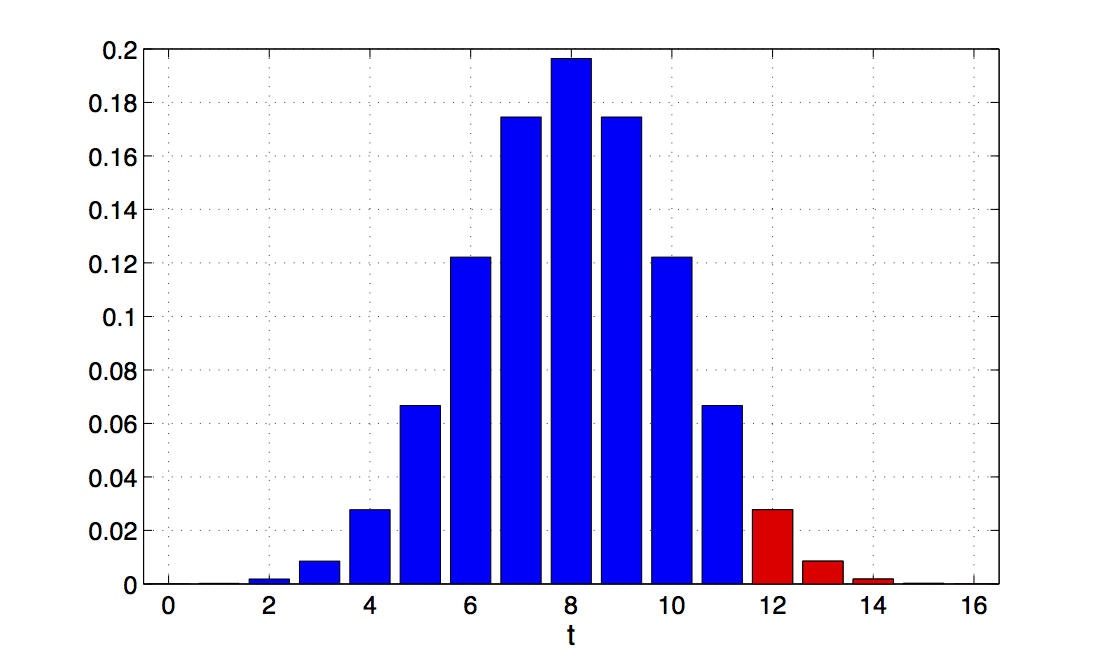
\includegraphics[height=0.6\textheight]{bond2.png}
	\end{center}
	$0.0384$~--- достигаемый уровень значимости при реализации $t=12$.
\end{frame}

\begin{frame}{Двусторонняя альтернатива}
%%%%%%%%%%%%%%%%%%%%%%%%%%%%%%%%%%%%%%%%%%%%%%%%%%%%%%%%%%%%%%%%%%%%%%%
%
%%%%%%%%%%%%%%%%%%%%%%%%%%%%%%%%%%%%%%%%%%%%%%%%%%%%%%%%%%%%%%%%%%%%%%%
	$H_1\colon$ Джеймс Бонд предпочитает какой-то определённый вид мартини.

	При справедливости такой альтернативы и большие, и маленькие значения $T$ свидетельствуют против $H_0$ в пользу $H_1$).

	Вероятность того, что Джеймс Бонд предпочтёт взболтанный мартини в~$\geq 12$ случаях из $16$ при справедливости $H_0$, равна $\frac{5034}{65536}\approx 0.0768$.
	\begin{center}
		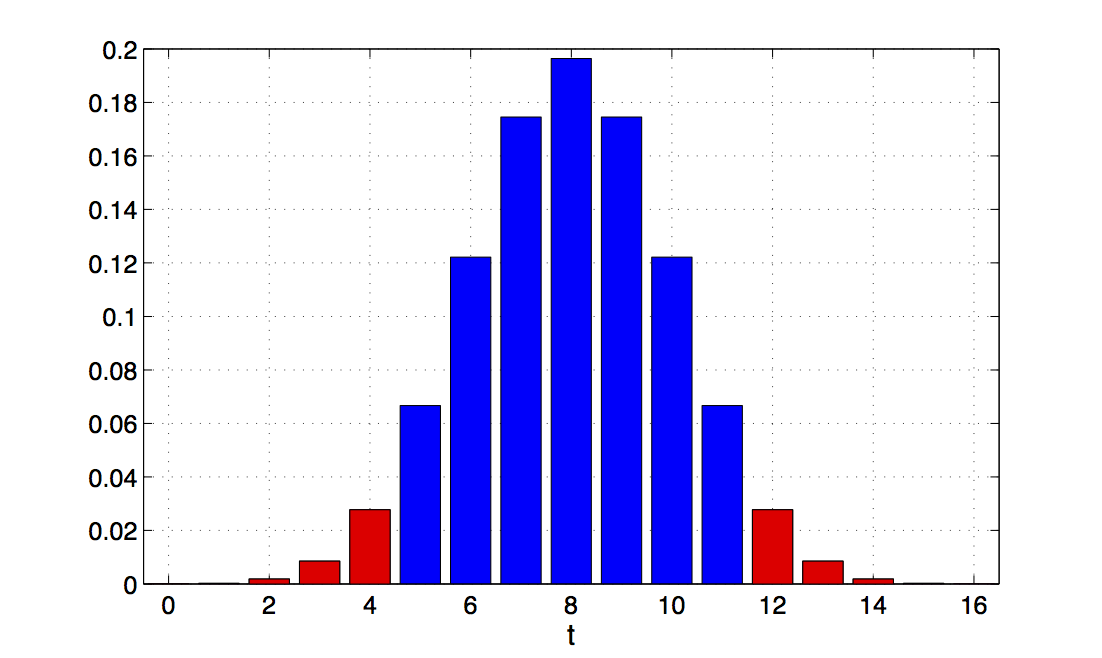
\includegraphics[height=0.6\textheight]{bond3.png}
	\end{center}
	$0.0768$~--- достигаемый уровень значимости при реализации $t=12$.
\end{frame}

\begin{frame}{Достигаемый уровень значимости}
%%%%%%%%%%%%%%%%%%%%%%%%%%%%%%%%%%%%%%%%%%%%%%%%%%%%%%%%%%%%%%%%%%%%%%%
%
%%%%%%%%%%%%%%%%%%%%%%%%%%%%%%%%%%%%%%%%%%%%%%%%%%%%%%%%%%%%%%%%%%%%%%%
		Чем ниже достигаемый уровень значимости, тем сильнее данные свидетельствуют против нулевой гипотезы в пользу альтернативы.

		\bigskip

		$0.0384$~--- вероятность реализации $t\geq 12$ при условии, что нулевая гипотеза справедлива, т.\,е. Джеймс Бонд выбирает мартини наугад.

		\bigskip

		Ещё раз: это не вероятность справедливости нулевой гипотезы!

\bigskip

		\textbf{Пример:} пусть Джеймс Бонд выбирает взболтанный мартини в $51$\% случаев (ненаблюдаемая вероятность).

		\bigskip

		Пусть по итогам $100$ испытаний взболтанный мартини был выбран $49$ раз. Достигаемый уровень значимости против односторонней альтернативы~--- $p\approx 0.6178.$
		Нулевая гипотеза не отвергается, при этом сказать, что она верна, было бы ошибкой~--- Джеймс Бонд выбирает смешанный и взболтанный мартини не с одинаковыми вероятностями!
\end{frame}

\begin{frame}{Мощность}
%%%%%%%%%%%%%%%%%%%%%%%%%%%%%%%%%%%%%%%%%%%%%%%%%%%%%%%%%%%%%%%%%%%%%%%
% Предполагая значение параметра, относительно которого мы проверяем гипотезу, известным, мы можем построить распределение значений статистики при этом значении. Чтобы получить мощность, нужно просуммировать высоты всех столбиков, соответствующих значениям статистики, при которых нулевая гипотеза отвергается.
%%%%%%%%%%%%%%%%%%%%%%%%%%%%%%%%%%%%%%%%%%%%%%%%%%%%%%%%%%%%%%%%%%%%%%%
	\only<1>{
		Проверяя нулевую гипотезу против двусторонней альтернативы, мы отвергаем $H_0$ при $t\geq 13$ или $t \leq 3$, что обеспечивает достигаемый уровень значимости $p=0.0213\leq\alpha=0.05$.
		\begin{center}
			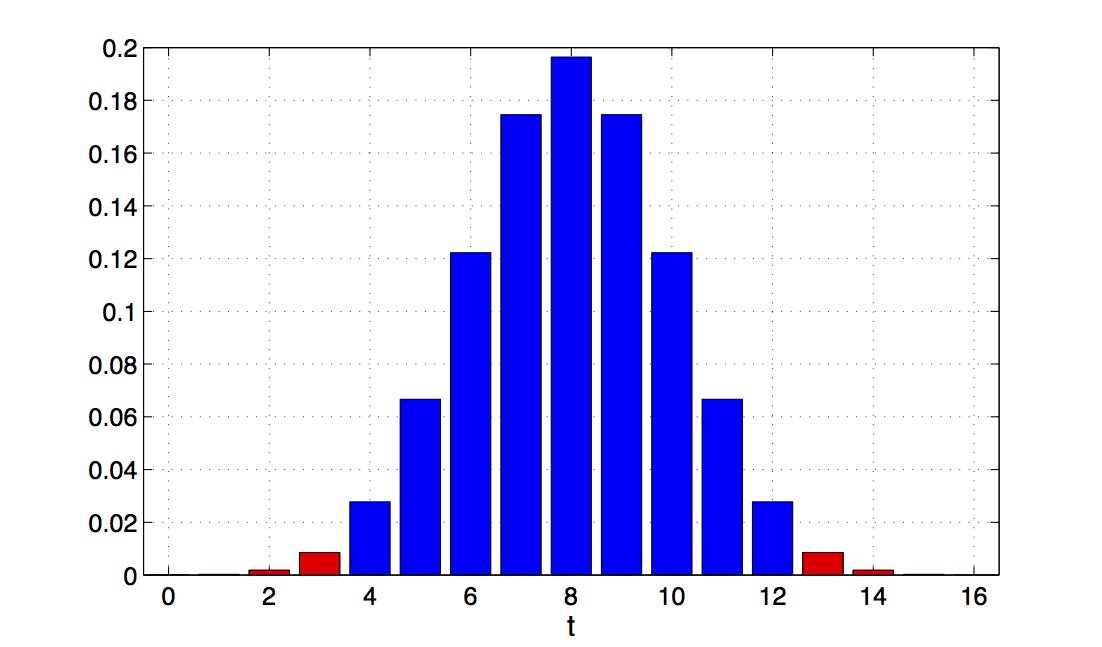
\includegraphics[height=0.3\textheight]{bond5.png}
		\end{center}
		Пусть Джеймс Бонд выбирает взболтанный мартини в $75$\% случаев.%    \vspace{-5pt}
		\begin{center}
			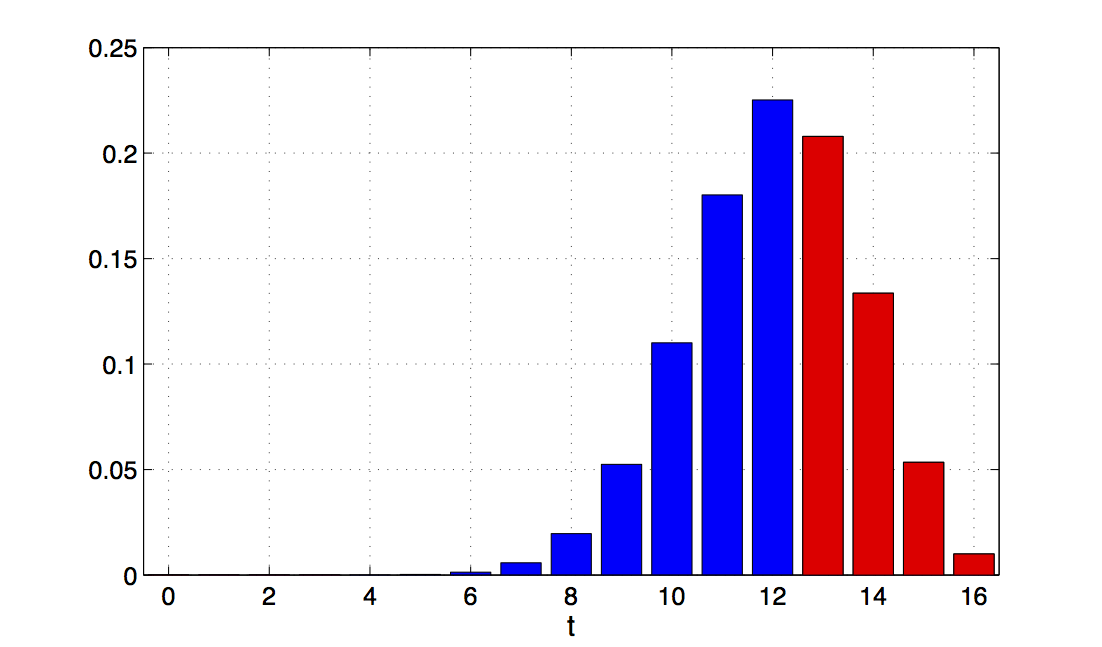
\includegraphics[height=0.3\textheight]{bond6.png}
		\end{center}
		$\pow \approx 0.6202,$ т.\,е., при многократном повторении эксперимента гипотеза будет отклонена только в $62$\% случаев.
	}

\only<2>{
	Мощность критерия зависит от следующих факторов:
	\begin{itemize}
		\item размер выборки
		\item размер отклонения от нулевой гипотезы
		\item чувствительность статистики критерия
		\item тип альтернативы
	\end{itemize}
}

	\only<3>{
%%%%%%%%%%%%%%%%%%%%%%%%%%%%%%%%%%%%%%%%%%%%%%%%%%%%%%%%%%%%%%%%%%%%%%%
% По этим кривым можно выбирать объём выборки, который нужен для обеспечения требуемой мощности
%%%%%%%%%%%%%%%%%%%%%%%%%%%%%%%%%%%%%%%%%%%%%%%%%%%%%%%%%%%%%%%%%%%%%%%
		\begin{center}
			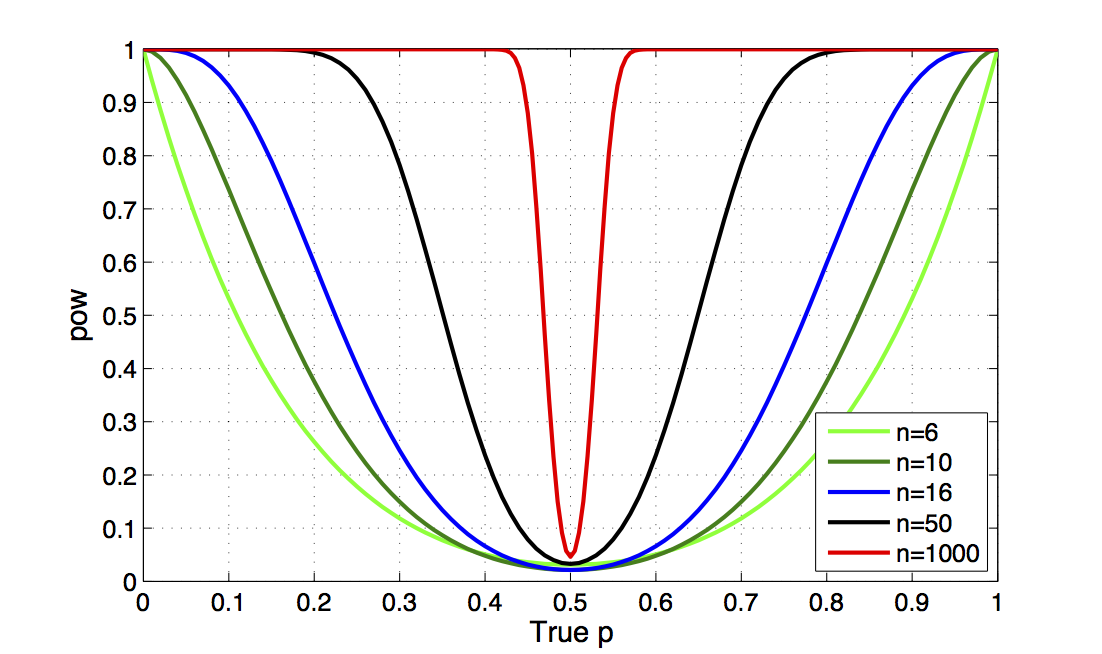
\includegraphics[width=0.8\textwidth]{powercurve.png}
		\end{center}
	}
\end{frame}

\begin{frame}{Размер выборки}
%%%%%%%%%%%%%%%%%%%%%%%%%%%%%%%%%%%%%%%%%%%%%%%%%%%%%%%%%%%%%%%%%%%%%%%
%
%%%%%%%%%%%%%%%%%%%%%%%%%%%%%%%%%%%%%%%%%%%%%%%%%%%%%%%%%%%%%%%%%%%%%%%
	Особенности прикладной задачи: $1$ порция мартини содержит $55$~мл джина и $15$~мл вермута~--- суммарно около $25$~мл спирта.
	Смертельная доза алкоголя при массе тела $80$~кг составляет от $320$ до $960$~мл спирта в~зависимости от толерантности (от $13$ до $38$ мартини).

	\bigskip

	Обеспечение требуемой мощности: размеры выборки подбирается так, чтобы при размере отклонения от нулевой гипотезы не меньше заданного (например, вероятность выбора взболтанного мартини не меньше $0.75$) мощность была не меньше заданной.
\end{frame}

\end{document}